\documentclass[11pt, final, a4paper]{book}
\usepackage{mathptmx}
\usepackage[latin1]{inputenc}
\usepackage[T1]{fontenc}
\usepackage[portuguese]{babel}
\usepackage{wasysym, textcomp}
\usepackage{indentfirst}
\usepackage{graphicx}
\usepackage{color}
\usepackage{soul}
\usepackage{float}
\usepackage{multicol}
\usepackage{eurosym}
\usepackage{enumitem}
\usepackage{caption}
\usepackage{subcaption}
\usepackage[final]{pdfpages}
\usepackage{subcaption}
\usepackage[pdftex]{hyperref}
\usepackage[top=2.5cm, bottom=2.5cm, inner=3cm, outer=2.5cm]{geometry}
\usepackage{fancyhdr}
\usepackage{booktabs}

\fancypagestyle{myplain}
{
	\fancyhf{}
	\renewcommand\headrulewidth{0pt}
	\renewcommand\footrulewidth{0pt}
	\fancyfoot[C]{\thepage}
}
\begin{document}
\pagenumbering{gobble}
\begin{center}
	\fbox{
	\begin{minipage}{.3\linewidth}
		\begin{flushleft}  
			\includegraphics[scale = 1]{Fotos/estg}
		\end{flushleft} 
	\end{minipage}
	\hfill
	\begin{minipage}{.6\linewidth}
		\begin{flushright}
			\centering                               
			{\large \vspace{.32cm} Instituto Polit�cnico de Leiria\par
			Escola Superior de Tecnologia e Gest�o\par
			Departamento de Engenharia Eletrot�cnica}
			\vspace{.18cm}
		\end{flushright} 
	\end{minipage}
}

\vspace{5.5cm}
{\LARGE\bfseries Sistema de Controlo e Comando Remoto (SiC2R)\par}

\vspace{6cm}
{\LARGE Christophe Filipe Pereira\par\vspace{0.4cm} Jos� Carlos Ribeiro Vieira \par}
\vfill
{\Large Leiria, julho de 2017\par}
\end{center}


\leavevmode\thispagestyle{empty}\newpage
\begin{titlepage}
	\centering
	\fbox{
		\begin{minipage}{.3\linewidth}
			\begin{flushleft}  
				\includegraphics[scale = 1]{Fotos/estg}
			\end{flushleft} 
		\end{minipage}
		\hfill
		\begin{minipage}{.6\linewidth}
			\begin{flushright}
				\centering                               
				{\large \vspace{.32cm} Instituto Polit�cnico de Leiria\par
					Escola Superior de Tecnologia e Gest�o\par
					Departamento de Engenharia Eletrot�cnica}
				\vspace{.18cm}
			\end{flushright} 
		\end{minipage}
	}

	
	\vspace{2.5cm}
	{\LARGE\bfseries Sistema de Controlo e Comando Remoto (SiC2R)\par}
	\vspace{0.7cm}
	
	{\Large Relat�rio final da Unidade Curricular de Projeto
		
		da Licenciatura em Engenharia Eletrot�cnica e de Computadores,
		
		ramo de Eletr�nica e Computadores\par}
	
	\vspace{3cm}
	{\LARGE Christophe Filipe Pereira\par\vspace{0.4cm} Jos� Carlos Ribeiro Vieira \par}
	\vfill
	{\Large Orientadores\par
		Lu�s Miguel Moreira Mendes (ESTG/IPLeiria)\par\vspace{0.3cm}
		Eng.~Celso Silva (Imporvia, Lda)}	
	\vfill
	{\Large Leiria, julho de 2017\par}
\end{titlepage}

\leavevmode\thispagestyle{empty}\newpage

\pagenumbering{roman}
\setcounter{page}{1}
\thispagestyle{empty}

\pagestyle{plain}
\vspace*{3cm}
\begin{flushright}
	\textit{Deixo um grande agradecimento\\ aos que me apoiaram neste percurso\\ acad�mico, nomeadamente, amigos,\\ professores e orientadores.\\\vspace{0.2cm}}
	\textbf{(Christophe Pereira)}\\
	\vspace{2cm}
	\textit{Dedico este trabalho\\ � minha fam�lia e a todos os que\\ me apoiaram e suportaram ao longo\\ do meu percurso acad�mico.\\\vspace{0.2cm}}
	\textbf{(Jos� Carlos Vieira)}\\
\end{flushright}
\thispagestyle{plain}
\chapter*{Agradecimentos}
\addcontentsline{toc}{chapter}{Agradecimentos}
\setlength{\parindent}{0pt}
Em primeiro lugar gostar�amos de agradecer ao Professor Lu�s Miguel Moreira Mendes, na qualidade de orientador deste projeto de licenciatura, por toda a ajuda prestada, disponibilidade e exig�ncia imposta, articulados sempre com boa disposi��o e um �timo ambiente de trabalho, e ao Engenheiro Celso Silva na qualidade de orientador pela ajuda prestada ao longo deste projeto, pela sua experi�ncia, aconselhamento e utiliza��o de regras de boas pr�ticas.\\[10pt]
Quer�amos prestar os nossos sinceros agradecimentos � Escola Superior de Tecnologia e Gest�o de Leiria (ESTG - IPLeiria) pelas instala��es, material facultado e possibilidade de estabelecer um bom ambiente de trabalho.\\[10pt]
Quer�amos de igual forma agradecer ao Centro de Eletr�nica da ESTG-IPLeiria, nomeadamente ao Eng.� Marco Santos e � Eng.� Sofia Gualdino, pela sua disponibilidade, tanto na aquisi��o de componentes como no fabrico de placas de circuito impresso, bem como em todas as outras solicita��es efetuadas.\\[10pt]
Por �ltimo, mas n�o menos importante, a todos os colegas de curso que nos auxiliaram e encorajaram ao longo de todo este percurso, os nossos sinceros agradecimentos.
\setlength{\parindent}{0.5pt}
\chapter*{Resumo}
\addcontentsline{toc}{chapter}{Resumo}
O presente relat�rio descreve todo o processo do desenvolvimento e implementa��o da unidade central de controlo e comando (U3C). A U3C � um equipamento eletr�nico de pequenas dimens�es, respons�vel pelo acionamento local ou remoto dos equipamentos perif�ricos (e.g., motores, l�mpadas, eletrov�lvulas) ligados a esta, quer seja da forma tradicional, via comando de radiofrequ�ncia, quer a partir de uma aplica��o \textit{Android} utilizando uma comunica��o GSM. Sendo esta desenvolvida para a empresa Imporvia, tem como principal objetivo a sua instala��o em caixas de motores de port�es autom�ticos residenciais e industriais.\\[6pt]

Neste documento apresenta-se a arquitetura do sistema implementado, sendo esta suficientemente flex�vel para que a U3C possa responder �s exig�ncias de futuros utilizadores, o modo de funcionamento, uma descri��o do desenvolvimento e implementa��o da unidade central, desde da sua especifica��o at� � sua vers�o industrial (final), o desenvolvimento das rotinas de programa��o e, por fim, os testes de funcionamento efetuados para avaliar o desempenho e robustez do sistema.\\[6pt]

A U3C permite o controlo e acionamento de automatismos de forma remota de duas formas independentes, via comando remoto de radiofrequ�ncia e via comunica��o GSM com uma interface gr�fica de uma aplica��o \textit{Android}. Disp�e de um conjunto de entradas e sa�das externas que permitem o uso de sensores e atuadores e ainda uma interface de configura��o local para a memoriza��o de comandos. A unidade central pode ser alimentada externamente a partir de uma fonte de corrente alternada ou corrente cont�nua. A U3C encontra-se pronta a ser comercializada e permite adaptabilidade � necessidade do utilizador, incluindo o uso de apenas um tipo de comunica��o, o uso das duas comunica��es e ter n�mero de entradas e sa�das vari�veis.\\[6pt]

\textbf{Palavras-chave: } Automatismos, Electr�nica anal�gica e digital, Microcontrolador, \textit{Transceivers} de radiofrequ�ncia, Banda ISM, GSM
\listoffigures
\addcontentsline{toc}{chapter}{Lista de figuras}
\listoftables
\addcontentsline{toc}{chapter}{Lista de tabelas}
\chapter*{Abreviaturas}
\addcontentsline{toc}{chapter}{Abreviaturas}

\begin{table}[H]
	\centering
	\small
	\begin{tabular}{lll}
		\toprule
		Sigla & Acr�nimo em portugu�s & Acr�nimo em ingl�s \\
		\midrule
		\textbf{3D} & Tridimensional & \textit{Three-Dimensional} \\
		\textbf{AFC} & Controlo Autom�tico de Frequ�ncia & \textit{Automatic Frequency Control} \\ 
		\textbf{ASK} & Comuta��o de Amplitude & \textit{Amplitude-Shift Keying} \\
		\textbf{AT} & Comandos de aten��o & \textit{Sttention Command} \\
		\textbf{BB} & Banda Base & \textit{Baseband} \\
		\textbf{BJT} & Trans�stor de Jun��o Bipolar & \textit{Bipolar Junction Transistor} \\ 
		\textbf{CI} & Circuito Integrado & \textit{Integrated Circuit} \\ 
		\textbf{EEPROM} & \hspace*{2.5cm} - - & \textit{Electrically-Erasable Programmable } \\
		& & \textit{Read-Only Memory}\\  
		\textbf{FIFO} & \hspace*{2.5cm} - - & \textit{First In, First Out} \\
		\textbf{GPRS} & Servi�o Geral de Pacotes por R�dio & \textit{General Packet Radio Service} \\
		\textbf{GSM} & Sistema Global para Comunica��es & \textit{Global System for Mobile} \\
		& M�veis & \textit{Communications}\\
		\textbf{IEEE} & \hspace*{2.5cm} - - & \textit{Institute of Electrical} \\
		& & \textit{and Electronics Engineers} \\
		\textbf{IF} & Frequ�ncia Interm�dia & \textit{Intermediate Frequency} \\
		\textbf{iOS} & Sistema Operativo \textit{IPhone} & \textit{Iphone Operating System} \\
		\textbf{ISM} & Industrial, Cient�fico e M�dico & \textit{Industrial, Scientific and Medical} \\
		\textbf{LED} & Diodo Emissor de Luz & \textit{Light Emitting Diode} \\
		\textbf{MOSFET} & Transistor de Efeito de Campo Metal & \textit{Metal Oxide Semiconductor Field} \\ 
		& & \textit{Effect Transistor}\\ 
		\textbf{OOK} & Modula��o Digital de Amplitude & \textit{On-Off Keying} \\
		\textbf{PC} & Computador Pessoal & \textit{Personal Computer} \\
		\textbf{PCI} & Placa de Circuito Impresso & \textit{Printed Circuit Board} \\
		\textbf{PDU} & Unidade de Dados de Protocolo & \textit{Protocol Data Unit} \\
		\textbf{PLL} & Malha de Captura de Fase & \textit{Phase-Locked Loop} \\
		\textbf{PWM} & Pulso com Modela��o & \textit{Pulse-Width Modulation} \\
		\textbf{RF} & Radiofrequ�ncia & \textit{Radio Frequency} \\
		\textbf{RGB} & Vermelho, Verde e Azul & \textit{Red, Green, and Blue} \\
		\textbf{RSSI} & Indicador de Pot�ncia do Sinal Recebido & \textit{Received Signal Strength Indicator} \\
		\textbf{RTC} & Rel�gio em Tempo Real & \textit{Real Time Clock} \\
		\textbf{SiC2R} & Sistema de Controlo e Comando Remoto & \textit{Control and Remote Control System} \\
		\textbf{SIM} & M�dulo de Identidade do Assinante & \textit{Subscriber Identity Module} \\
		\textbf{SMD} & Componente de Montagem Superficial & \textit{Surface Mounting Device} \\
		\textbf{SMS} &  Servi�o de Mensagens Curtas & \textit{Short Message Service} \\
		\textbf{SPI} & Interface Perif�rica Serial  & \textit{Serial Peripheral Interface} \\
		\textbf{TQFP} & \hspace*{2.5cm} - - & \textit{Thin Quad Flat Package} \\
		\textbf{U3C} & Unidade Central de Controlo e Comando & \textit{Central Control and Command Unit} \\
		\textbf{UART} & Recetor/Transmissor S�ncrono Universal & \textit{Universal Synchronous Receiver/} \hspace*{1cm}\\
		& & \textit{Transmitter}\\  
		\textbf{UHF} & Frequ�ncia Ultra-Alta & \textit{Ultra High Frequency} \\
		\textbf{USB} & Comunica��o Serie Universal & \textit{Universal Serial Bus} \\
		\textbf{VNA} & Analizador Vectorial & \textit{Vector Network Analyzers} \\
		\bottomrule
	\end{tabular}
\end{table}
\tableofcontents
\vfill\pagebreak\leavevmode\newpage\thispagestyle{headings}

\pagestyle{headings}
\pagenumbering{arabic}
\chapter{Introdu��o}\label{introducao}
Neste cap�tulo apresenta-se o contexto e a motiva��o que levaram ao desenvolvimento e realiza��o de uma unidade de controlo e comando de automatismos. S�o apresentados tamb�m os principais objetivos e cen�rios de aplica��o. A organiza��o do documento e ainda as contribui��es tecnol�gicas s�o tamb�m apresentadas no final do cap�tulo.
\section{Motiva��o e contexto}
Com o evoluir da sociedade, os cidad�os cada vez t�m menos tempo e disposi��o para a realiza��o de pequenas tarefas do seu dia-a-dia, quer estas sejam de �mbito pessoal ou familiar. Por exemplo, nas sociedades modernas, as pessoas muitas das vezes n�o t�m disponibilidade temporal para chamar um t�cnico a casa e esperar que o trabalho termine ou, por exemplo, acionar o sistema de rega e esperar que este termine. Para al�m das quest�es relacionadas com a disponibilidade temporal dos cidad�os, por vezes tamb�m n�o existem interfaces que facilitem a execu��o de tarefas repetitivas, como � caso da ativa��o do sistema de aquecimento/arrefecimento da habita��o quando se sai do trabalho, para que, ao chegar a casa, o cidad�o encontre a temperatura desejada, ou de um sistema autom�tico para abertura e fecho de estores a partir de um sensor de luminosidade ou ainda a ativa��o do sistema de rega tendo em conta a humidade do solo e n�o em hor�rio de rega pr�-definido. \\[6pt]
O avan�o tecnol�gico verificado nos �ltimos anos, tem vindo a revolucionar, alguns aspetos da vida quotidiana dos cidad�os. O papel da evolu��o tecnol�gica � facilitar a vida dos cidad�os e conseguir proporcionar-lhes uma melhor gest�o do seu tempo. Um exemplo pr�tico desse papel da tecnologia � a possibilidade de utilizar um simples \textit{smartphone} para comunicar e trocar informa��es e documentos com pessoas do todo o mundo, consultar hor�rios dos transportes, o tr�nsito, marcar consultas, fechar neg�cios, entre outros. Este desenvolvimento tecnol�gico nos dias de hoje, permite �s pessoas interagir umas com as outras independentemente da dist�ncia, local e hora.\\[6pt]
No seguimento do avan�o tecnol�gico foram desenvolvidos os \textit{smartphones}. A venda global deste tipo de dispositivos tem aumentado ao longo dos anos e a tend�ncia � que este n�mero cres�a. Segundo o portal de estat�sticas Statista, e como apresentado na figura \ref{fig:estatiscasmartphone}, o n�mero de \textit{smartphones} existentes em todo o mundo em 2014 era de 1.57 mil milh�es. Desde ent�o at� o presente ano, 2017, o n�mero aumentou cerca de 0.75 mil milh�es, apontando assim para os 2.32 mil milh�es. Ainda, n�meros estat�sticos apontam para a exist�ncia de 2.87 mil milh�es de dispositivos m�veis \textit{smartphones} no ano de 2020. Isto significa que tendencialmente as pessoas compram este tipo de dispositivos e os levam consigo para todo o lado.\\[6pt]
A tecnologia que o mercado oferece para este tipo de sistemas � essencialmente composta por recetor de radiofrequ�ncia (RF) que ao receber o c�digo de um comando remoto, faz acionar ou n�o o mecanismo, normalmente port�es, consoante a sua exist�ncia em mem�ria ou n�o. A seguran�a e robustez destes sistemas � �tima, contudo n�o conseguem a flexibilidade e adaptabilidade necess�rias.\\[6pt]
\begin{figure}[H]
	\centering
	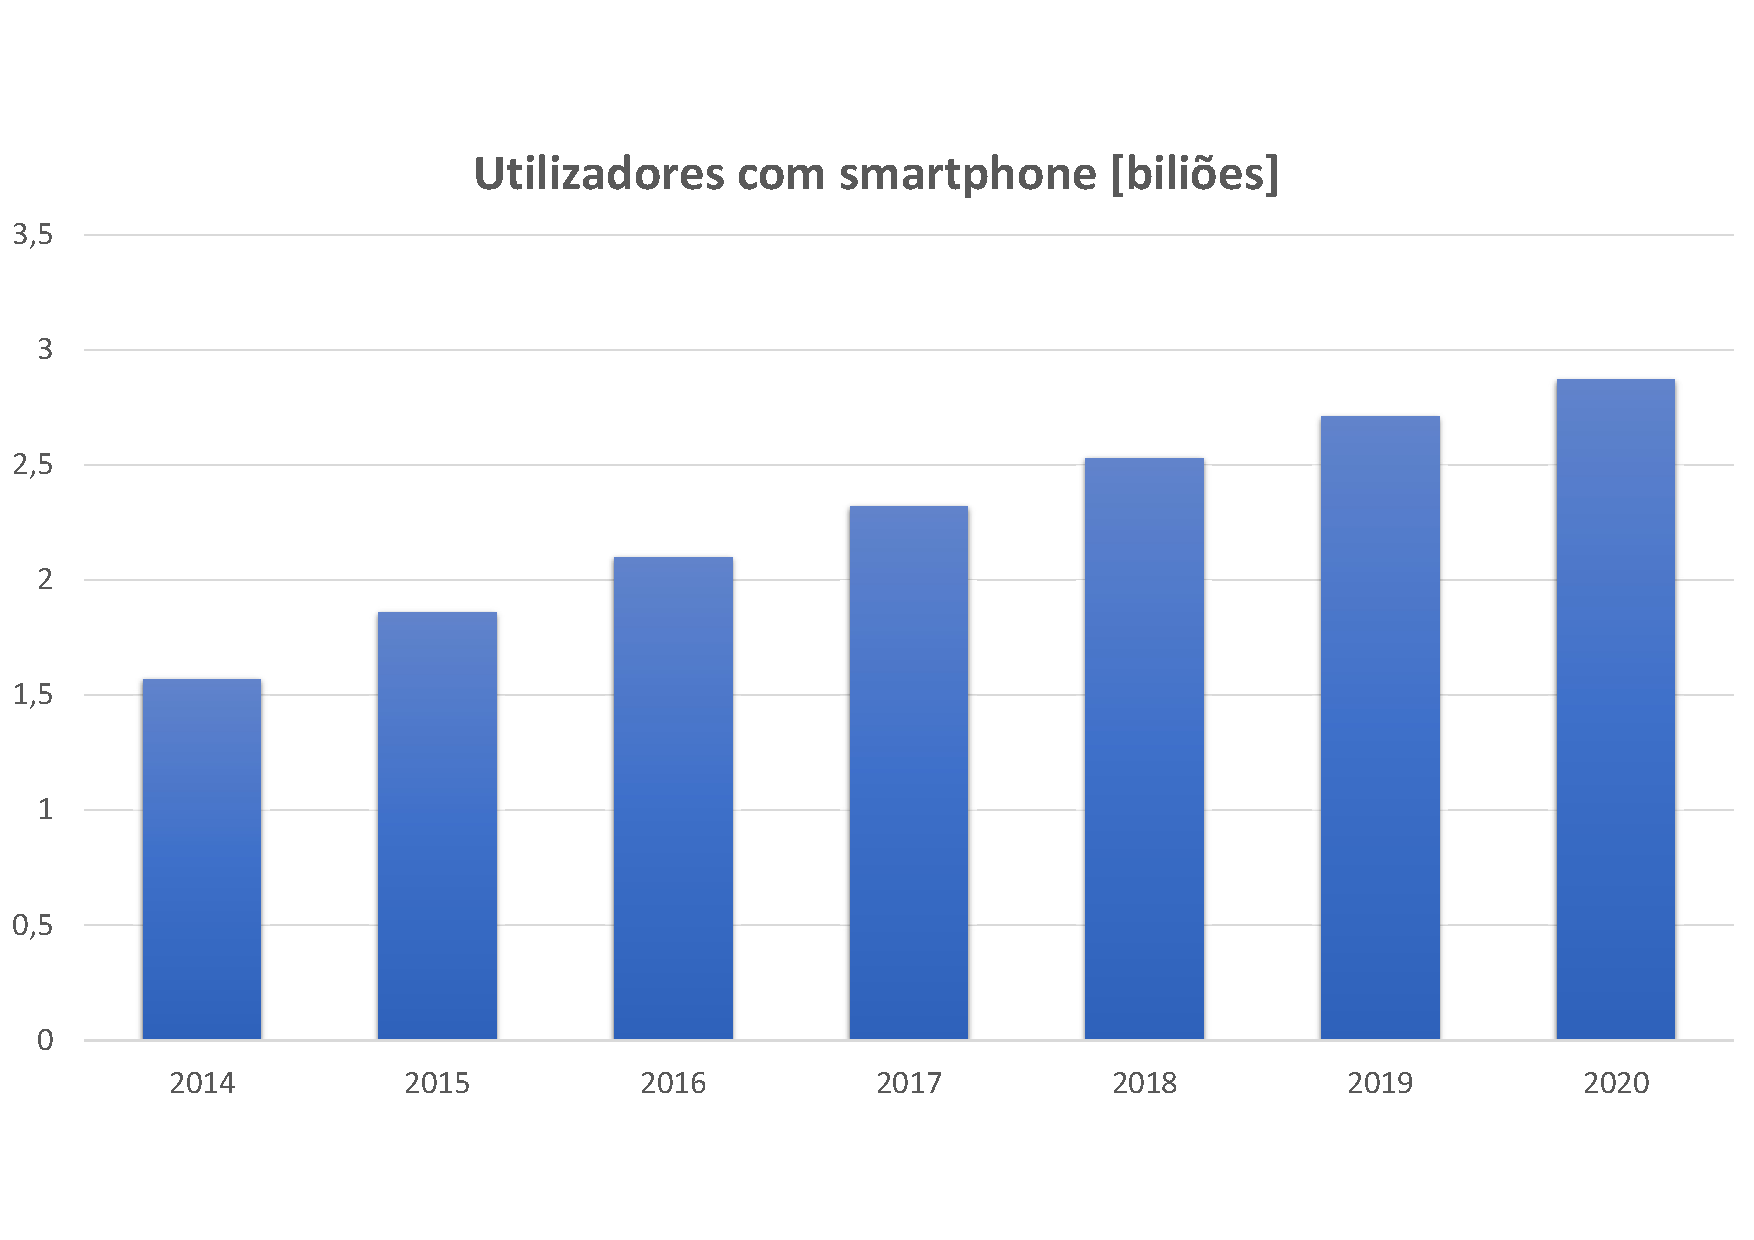
\includegraphics[clip, trim=0cm 1.5cm 0cm 1.5cm, width=0.71\linewidth]{Figuras/estatiscasmartphone}
	\caption{N�mero de utilizadores de \textit{smartphones} em todo o mundo entre 2014 e 2020 [\ref{estatiscasmart}].}
	\label{fig:estatiscasmartphone}
\end{figure}
Sendo o pedido de atua��o realizado atrav�s de comandos remotos alimentados por uma pilha, a pot�ncia emitida � baixa para que esta dure bastante tempo (tipicamente 1 a 2 anos), pelo que a dist�ncia � relativamente baixa e n�o servir� para acionamentos a grandes dist�ncias.\\[6pt]
Outro ponto negativo destes sistemas � relativo �s interfaces disponibilizadas. Estes, normalmente, n�o fazem uso de sensores externos ao sistema, isto �, os �nicos sensores utilizados s�o internos, como � o caso dos sensores de infravermelhos para detetar objetos na trajet�ria da abertura/fecho do port�o que far�o comutar o estado de funcionamento dos motores. Contudo, se for necess�rio atuar o sistema por efeito de algum acontecimento (e.g., gerado por um sensor), n�o existe a interface. Para al�m disso o n�mero de sa�das � fixo e n�o escal�vel dependendo da finalidade. Isto tr�s implica��es a n�vel do custo, pois, por vezes � necess�rio pagar por interfaces que n�o s�o utilizadas.\\[6pt]
Desta forma a exist�ncia de aplica��es que tornam poss�veis a realiza��o de qualquer tipo de tarefas atrav�s de um simples \textit{click}, s�o importantes e do agrado dos utilizadores, oferecendo-lhes in�meras vantagens, como por exemplo: o aumento de qualidade de vida, redu��o de custos de deslocamentos, diminui��o de preocupa��es, maior tempo de lazer e conv�vio, entre outras.
\section{Objetivos}
Dentro do contexto referido na sec��o anterior, o trabalho apresentado neste projeto teve como objetivo geral a desenvolvimento e implementa��o de uma unidade central de controlo e comando (U3C), de baixo custo e elevada robustez para utiliza��o em automatismos de port�es residenciais e industriais. O sistema deve permitir o controlo local sem fios e remoto. Para isso, a U3C teria de permitir comunica��es na banda \textit{industrial, scientific and medical} (ISM) dos 433 MHz e na banda do \textit{global system for mobile communications} (GSM). Desta forma a U3C � capaz de acionar port�es, ou outros automatismos, de forma segura tanto da forma tradicional, via comando, como atrav�s de uma aplica��o \textit{Android}, mudando assim o conceito t�pico de um recetor de port�es. O m�dulo de alimenta��o de toda a unidade, a disponibiliza��o das v�rias entradas para uso de sensores e de v�rias sa�das para a atua��o dos sistemas desejados teriam tamb�m de ser desenvolvidos.\\[6pt]
A U3C ter� de funcionar em v�rios cen�rios de aplica��o distintos. Na figura \ref{fig:cenarios} est�o ilustrados alguns dos cen�rios de utiliza��o, tendo estes sido definidos considerando as poss�veis exig�ncias de futuros clientes do sistema.\\[6pt]
\begin{figure}[H]
	\centering
	\begin{subfigure}{.33\textwidth}
		\centering
		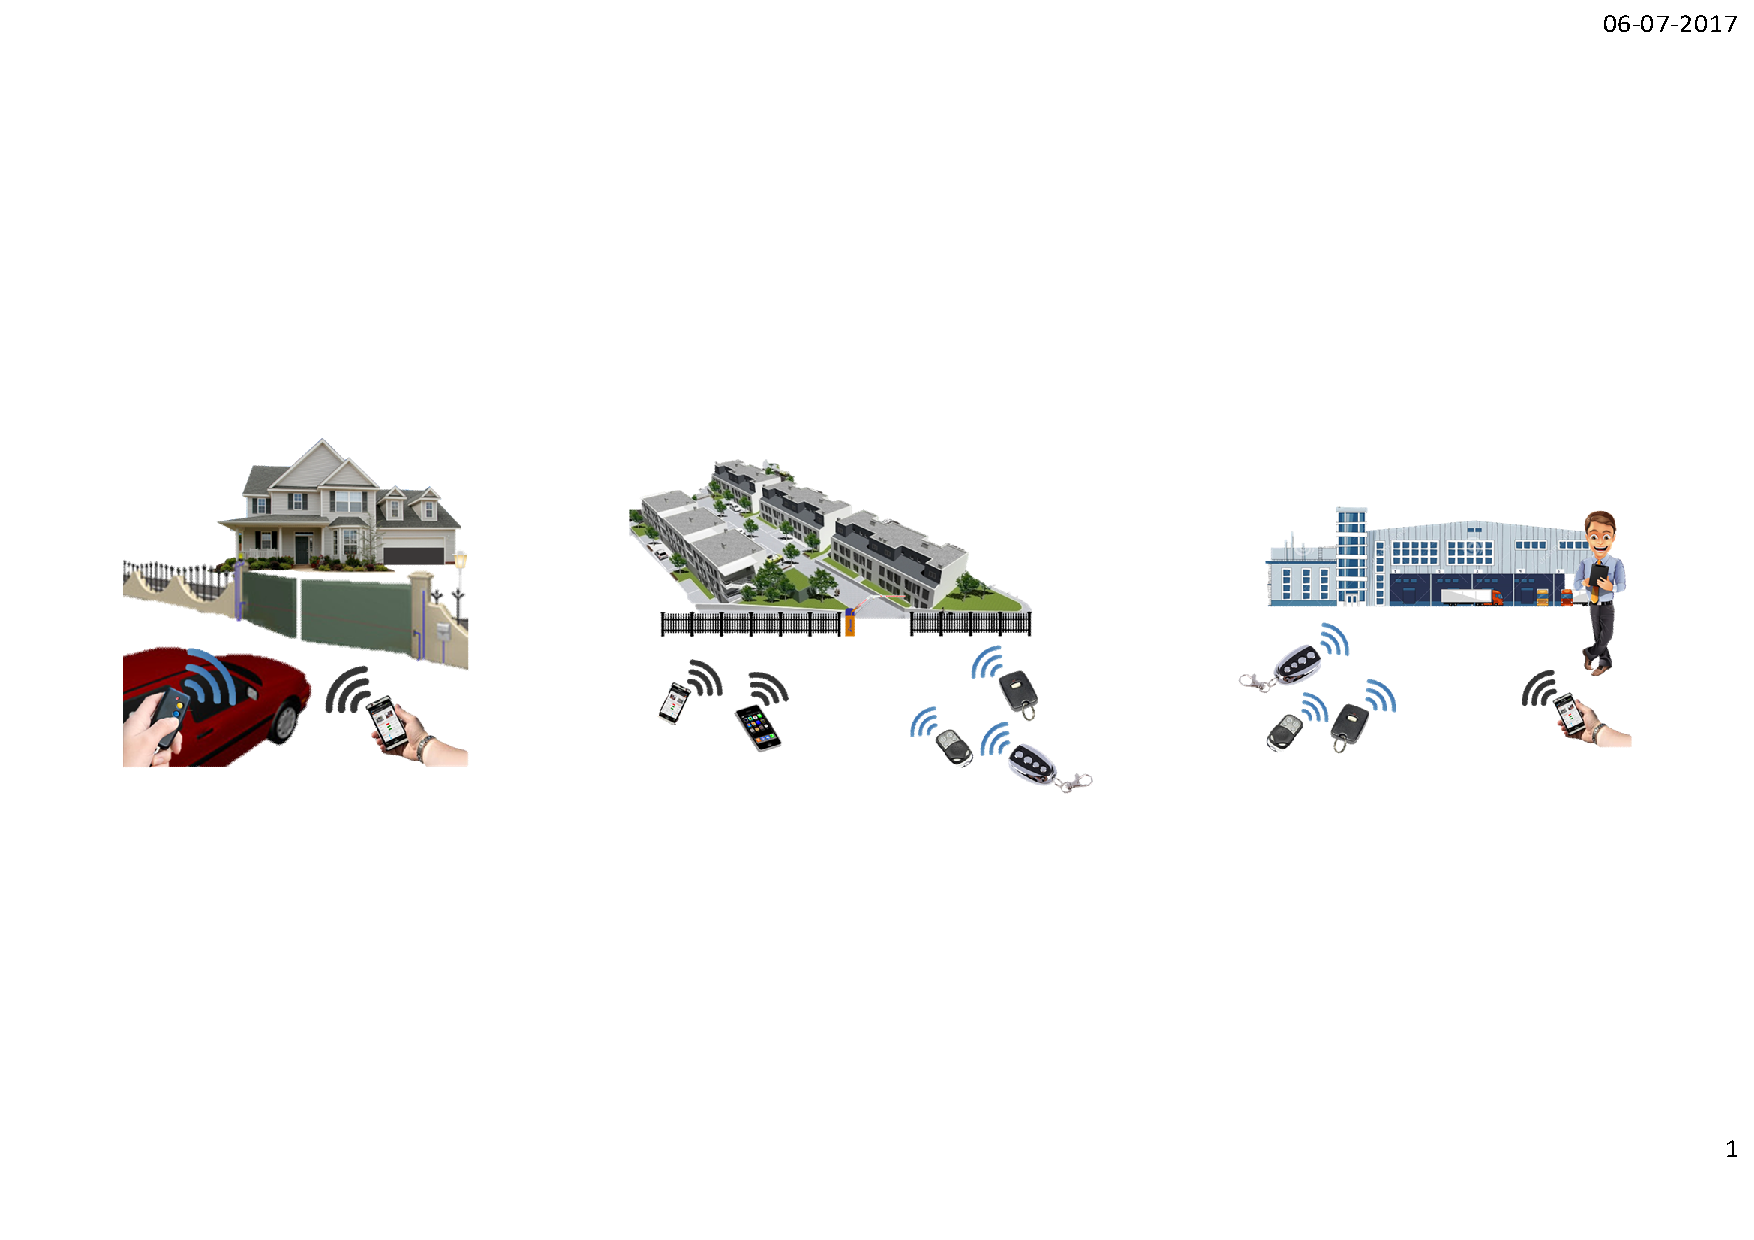
\includegraphics[clip, trim=1.5cm 7cm 21cm 7cm, width=0.78\linewidth]{Figuras/cenario}
		\captionsetup{labelformat=empty}
		\caption{(a) Habita��o individual.}
		\label{fig:cenariosa}
	\end{subfigure}%
	\begin{subfigure}{.33\textwidth}
		\centering
		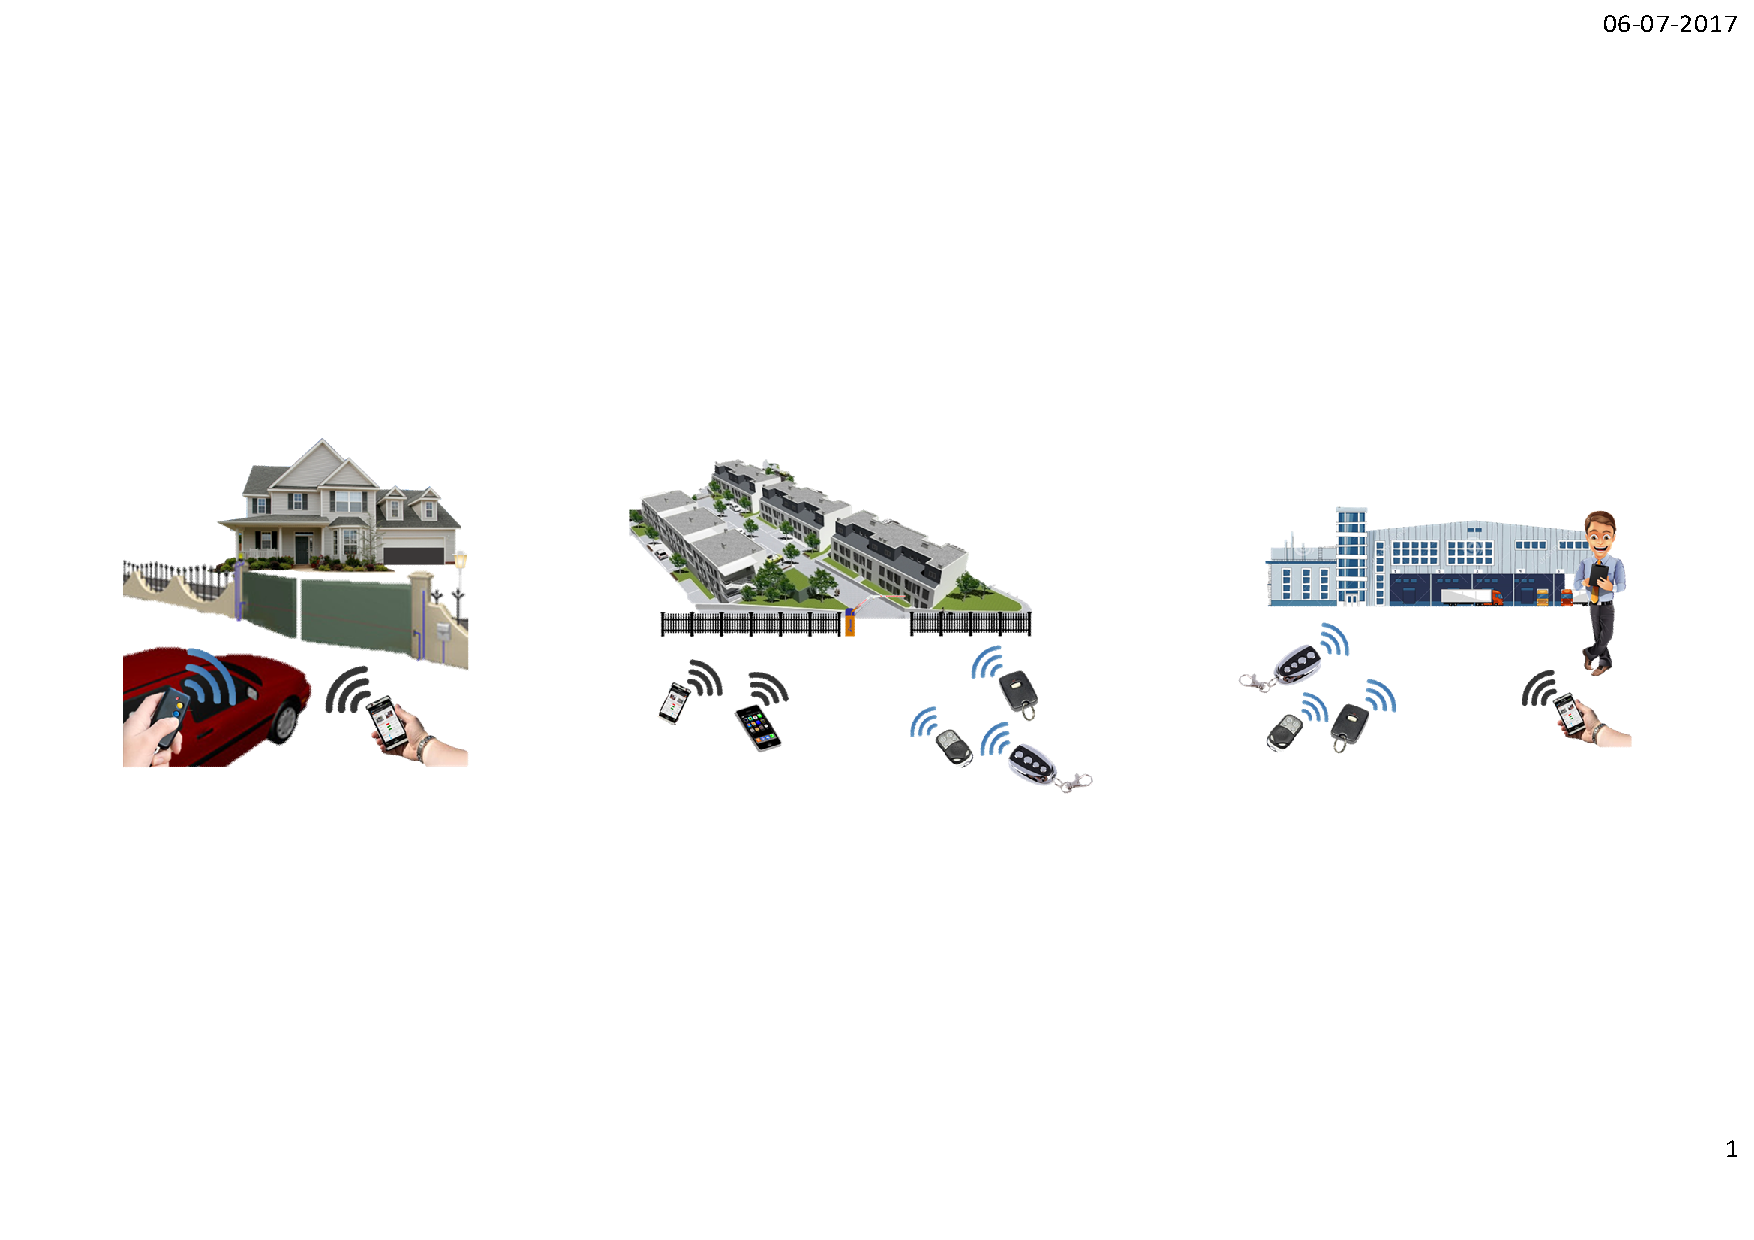
\includegraphics[clip, trim=10.5cm 7cm 10.8cm 7cm, width=0.91\linewidth]{Figuras/cenario}
		\captionsetup{labelformat=empty}
		\caption{(b) Habita��o coletiva.}
		\label{fig:cenariosb}
	\end{subfigure}
	\begin{subfigure}{.33\textwidth}
		\centering
		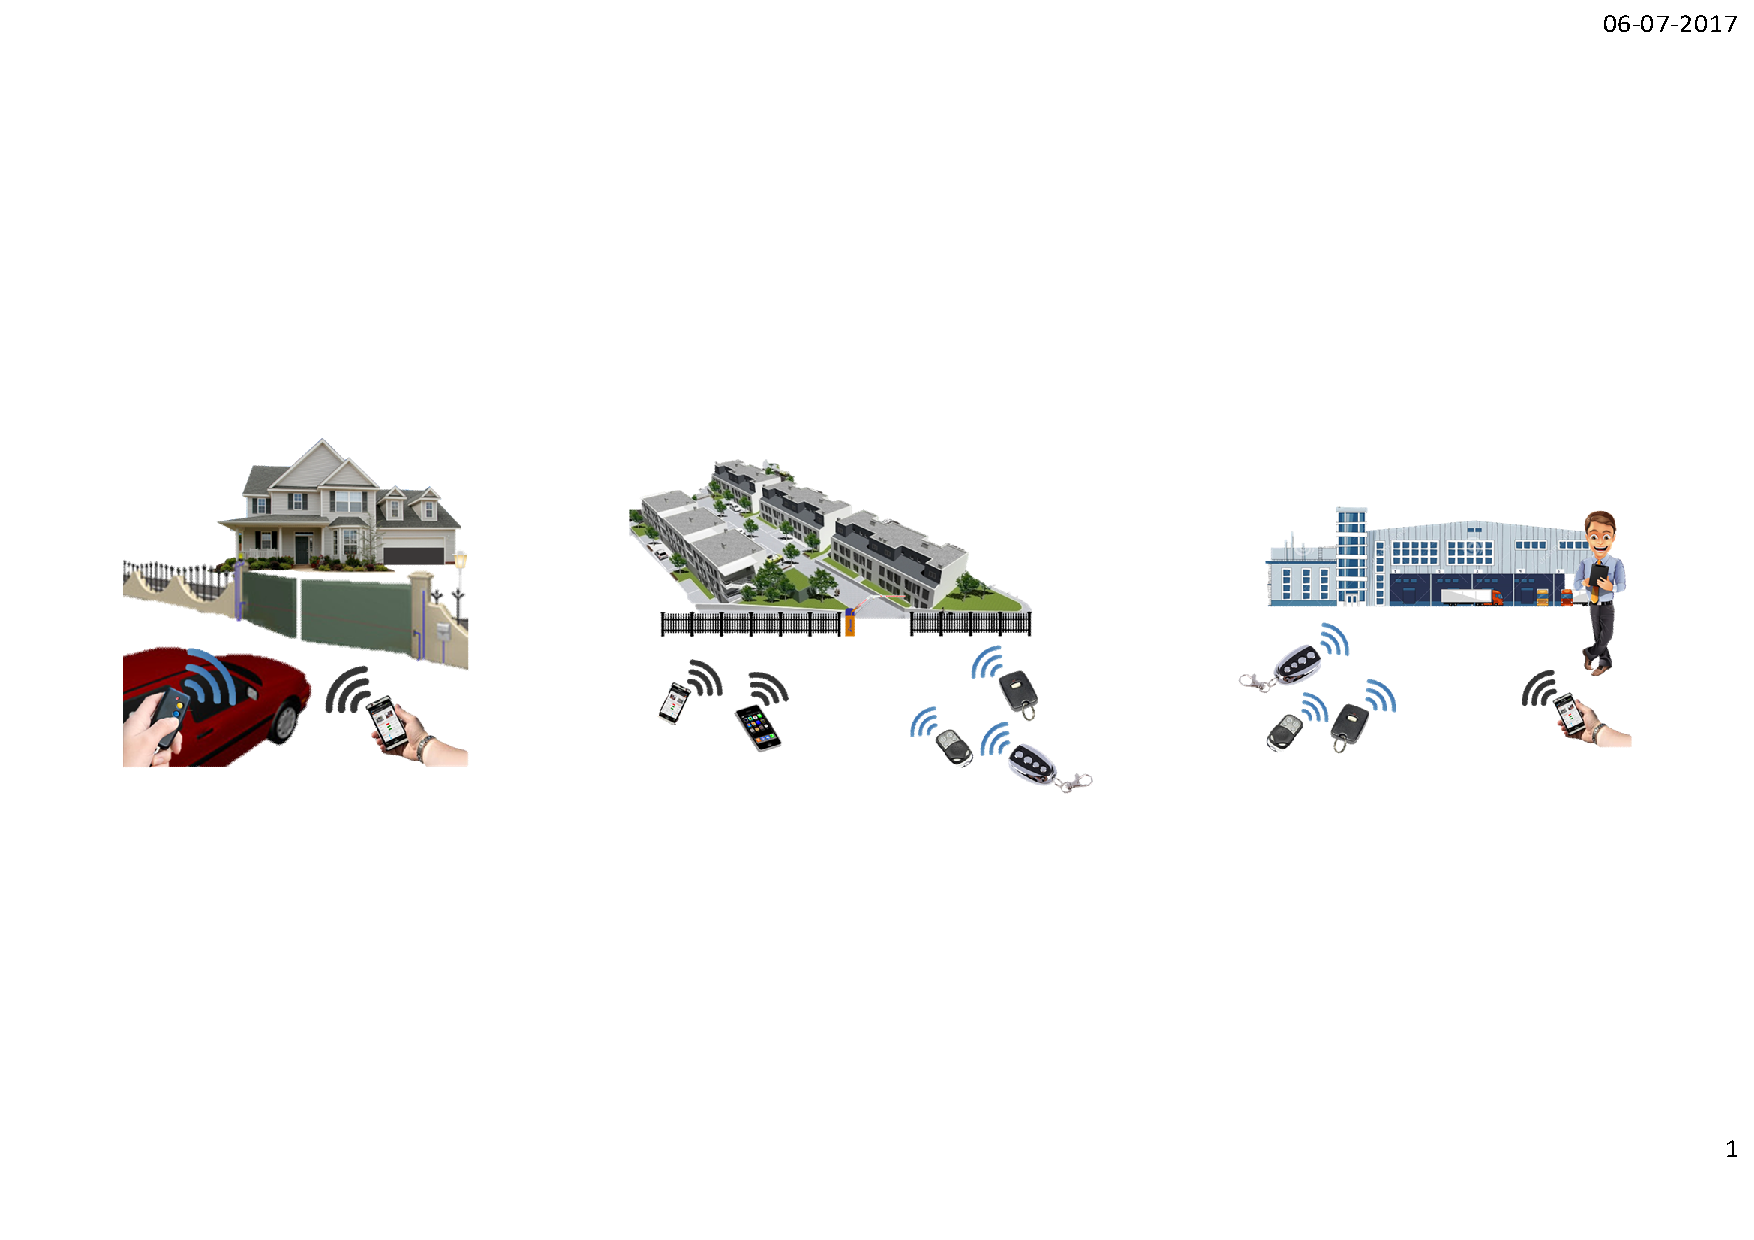
\includegraphics[clip, trim=20.5cm 7cm 1.7cm 7cm, width=0.805\linewidth]{Figuras/cenario}
		\captionsetup{labelformat=empty}
		\caption{(c) Pequena/m�dia empresa.}
		\label{fig:cenariosc}
	\end{subfigure}
	\caption{Cen�rios de aplica��o.}
	\label{fig:cenarios}
\end{figure}
Na ilustra��o mostrada na figura \ref{fig:cenariosa} o cen�rio de utiliza��o � relativo a uma moradia individual em que o n�mero de comandos remotos e dispositivos \textit{Android} � reduzido. Nesta tipologia de utiliza��o os mecanismos a acionar ser�o port�es, sistemas de ilumina��o, rega, entre outros. Neste caso o controlo das entradas e sa�das n�o ser� o foco principal, no entanto ter� de ter essa possibilidade. No caso de uma habita��o coletiva ou de um condom�nio, tal como mostrado na figura \ref{fig:cenariosb}, � importante a exist�ncia de um recetor universal, visto que existir�o muitos utilizadores, com diferentes comandos remotos ou de fabricantes diferentes. Nesta situa��o � tamb�m importante, a utiliza��o dos \textit{smartphones} para ativa��o dos automatismos ligados ao recetor universal, e a grava��o do hist�rico dos acessos para seguran�a. Por �ltimo, na terceira situa��o (figura \ref{fig:cenariosc}) que corresponde ao caso de uma pequena/m�dia empresa, onde o n�mero de utilizadores pode ser elevado, poder� existir a necessidade de impor restri��es de hor�rios individuais ou coletivos que ser� gerido/controlado pelo administrador da U3C.

\section{Contribui��es tecnol�gicas}
A unidade desenvolvida providencia a possibilidade do acionamento de mecanismos que se encontram ligados a esta de forma remota, tanto via comando RF como via aplica��o \textit{Android} atrav�s de uma comunica��o GSM.\\[6pt]
Na pesquisa inicial, que tinha como intuito a an�lise de v�rias unidades centrais existentes no mercado, foram abordadas unidades que implementam o acionamento via comando remoto, e outros via GSM (apenas uma marca), no entanto n�o houve conhecimento da exist�ncia de unidades com ambos os m�todos de comunica��o. Assim, o produto � considerado inovador e uma mais valia n�o s� para a empresa Imporvia, melhorando o seu posicionamento a n�vel do mercado nacional e internacional deste ramo, bem como aos utilizadores, onde lhes s�o oferecidas in�meras vantagens da sua utiliza��o.

\section{Organiza��o do documento}
Para que o objetivo principal fosse alcan�ado, foram estabelecidos v�rios objetivos espec�ficos. Inicialmente, seria necess�rio realizar uma pesquisa de mercado para identificar os equipamentos existentes que d�o resposta a este tipo de sistemas e a determina��o das suas principais carater�sticas. Posteriormente, a analise dos cen�rios de aplica��o em que a U3C se poderia enquadrar e a arquitetura necess�ria implementar para responder �s suas poss�veis exig�ncias. Ap�s este processo, seria cumprida a an�lise de mercado referente � tecnologia necess�ria para a implementa��o desta arquitetura, designadamente na vertente da engenharia: microcontroladores, m�dulos GSM, m�dulos transcetores de RF, mem�rias, fontes comutadas, rel�s, etc.\\[6pt]
Com esse trabalho elaborado seria desenvolvido a placa de circuito impresso (PCI) e as rotinas de programa��o da U3C para que pudesse cumprir os objetivos propostos. Finalmente, o projeto seria terminado com a elabora��o de toda a sua documenta��o. Para isso a descri��o do desenvolvimento e implementa��o da U3C � feito ao longo dos 6 cap�tulos deste relat�rio. No primeiro cap�tulo s�o introduzidos os temas principais do trabalho, fazendo-se o respetivo enquadramento, e apresentando-se objetivos, cen�rios de aplica��o e as contribui��es tecnol�gicas.\\[6pt]

No cap�tulo 2 s�o apresentados os sistemas de controlo de automatismos existentes no mercado atual e disponibilizados pelas marcas mais relevantes desta �rea t�cnica. As v�rias tecnologias, modos de funcionamento e as caracter�sticas t�cnicas desses sistemas comerciais s�o tamb�m discutidos. Para al�m disso, s�o apresentados e especificados os dois tipos de c�digos mais utilizados neste tipo de sistemas. Ainda neste cap�tulo, � dada a conhecer a arquitetura do sistema, que inclui as especifica��es e funcionalidades da U3C, apresentando um diagrama modelar e respetiva descri��o.\\[6pt]

O terceiro cap�tulo apresenta e descreve o desenvolvimento da U3C. Para cada m�dulo funcional interna da U3C � apresentado um diagrama funcional, � feita uma descri��o das funcionalidades pretendidas, e apresentados os circuitos eletr�nicos associados.
No cap�tulo 4 s�o dadas a conhecer as PCI desenvolvidas para a implementa��o dos circuitos eletr�nicos projetados. S�o tamb�m apresentas as especifica��es t�cnicas, as normas consideradas para o desenvolvimento das placas e os planos de massa. Por �ltimo � apresentado o aspeto final do sistema.\\[6pt]

O cap�tulo cinco descreve o desenvolvimento da programa��o da unidade central. S�o apresentadas as rotinas de programa��o tanto do m�dulo GSM como do m�dulo RF. Neste cap�tulo � apresentado o desenvolvimento da aplica��o \textit{Android} que serve de interface bidirecional entre o utilizador e a U3C.\\[6pt]

Este relat�rio termina com o cap�tulo 6. O cap�tulo inicia com a apresenta��o dos testes de verifica��o do funcionamento da U3C, onde as diversas medidas de consumos, temperaturas e integridade das alimenta��es e sinais s�o apresentados. O cap�tulo termina com a apresenta��o das poss�veis melhorias a introduzir no sistema.\\[6pt]
\vfill\thispagestyle{plain}
\pagestyle{headings}
\chapter{Arquitetura da unidade central}
Neste cap�tulo s�o apresentados os sistemas de controlo de automatismos comerciais dispon�veis no mercado, tanto ao n�vel dos transmissores como dos recetores, e descritas as suas caracter�sticas t�cnicas principais. Para al�m disso, s�o enumerados e descritos o tipo de c�digo mais utilizados neste tipo de sistemas e mostradas as principais caracter�sticas e a composi��o da trama de um c�digo fixo e de um \textit{rolling code}. O cap�tulo termina com a defini��o e descri��o da arquitetura do sistema a implementar. Esta foi desenvolvida tendo em conta as caracter�sticas e funcionalidades dos dispositivos existentes no mercado e os cen�rios de aplica��o apresentados e descritos no cap�tulo anterior.
\section{Sistema de controlo de automatismos comerciais}
Um sistema de controlo de automatismos residenciais e industriais � composto por dois subsistemas: os transmissores (comandos remotos) e os recetores (unidades de controlo e comando). Quando um dos bot�es do comando � acionado, este transmite um sinal que � composto por um dado c�digo identificativo do comando e do bot�o/canal. Posteriormente, recetor deteta esse sinal e recupera a informa��o contida nele. Ap�s a verifica��o da sua exist�ncia em mem�ria, pressionado o automatismo do canal que lhe est� alocado.\\[6pt] 
Atualmente existem diversas marcas/fabricantes que disponibilizam sistemas de controlo de automatismos residenciais e industriais. As subsec��es seguintes apresentam alguns dos equipamentos desenvolvidos por algumas dessas empresas e descrevem tamb�m algumas das caracter�sticas principais desses equipamentos. Esta an�lise de mercado � essencial pois para a conce��o de um novo produto � importante que as especifica��es e funcionalidades definidas para o novo equipamento sejam superiores �s dos produtos j� existentes no mercado. S� assim a introdu��o de um novo equipamento pode ter sucesso comercial e ser concorrente com as demais solu��es dispon�veis. 
\subsection{Unidades transmissoras}
Na tabela \ref{fig:tx} est�o indicados alguns transmissores (comandos remotos) comerciais e algumas das suas caracter�sticas t�cnicas principais. Como � poss�vel observar, a frequ�ncia central dos sinais transmitidos pelos comandos � de 433 MHz ou de 868 MHz (bandas ISM), sendo contudo a primeira a mais utilizada. Outra caracter�stica importante que se conseguiu obter, foi o tipo de codifica��o utilizado pelos v�rios comandos. Estes geralmente utilizam os c�digos fixos ou os \textit{rolling codes}. Pela tabela verifica-se ainda que a dist�ncia de transmiss�o est� entre os 50 m e os 150 m. Esta dist�ncia � obtida em espa�o livre e depende muito do recetor utilizado (depende da sensibilidade do recetor).\\[6pt]
Na figura \ref{fig:comandosmarcas} s�o apresentados alguns exemplos de comandos remotos existentes no mercado, nela pode-se verificar, tal como na tabela dos transmissores, que o n�mero de bot�es dispon�veis � vari�vel (tipicamente entre de 2 a 4).
\begin{table}[H]
	\centering
	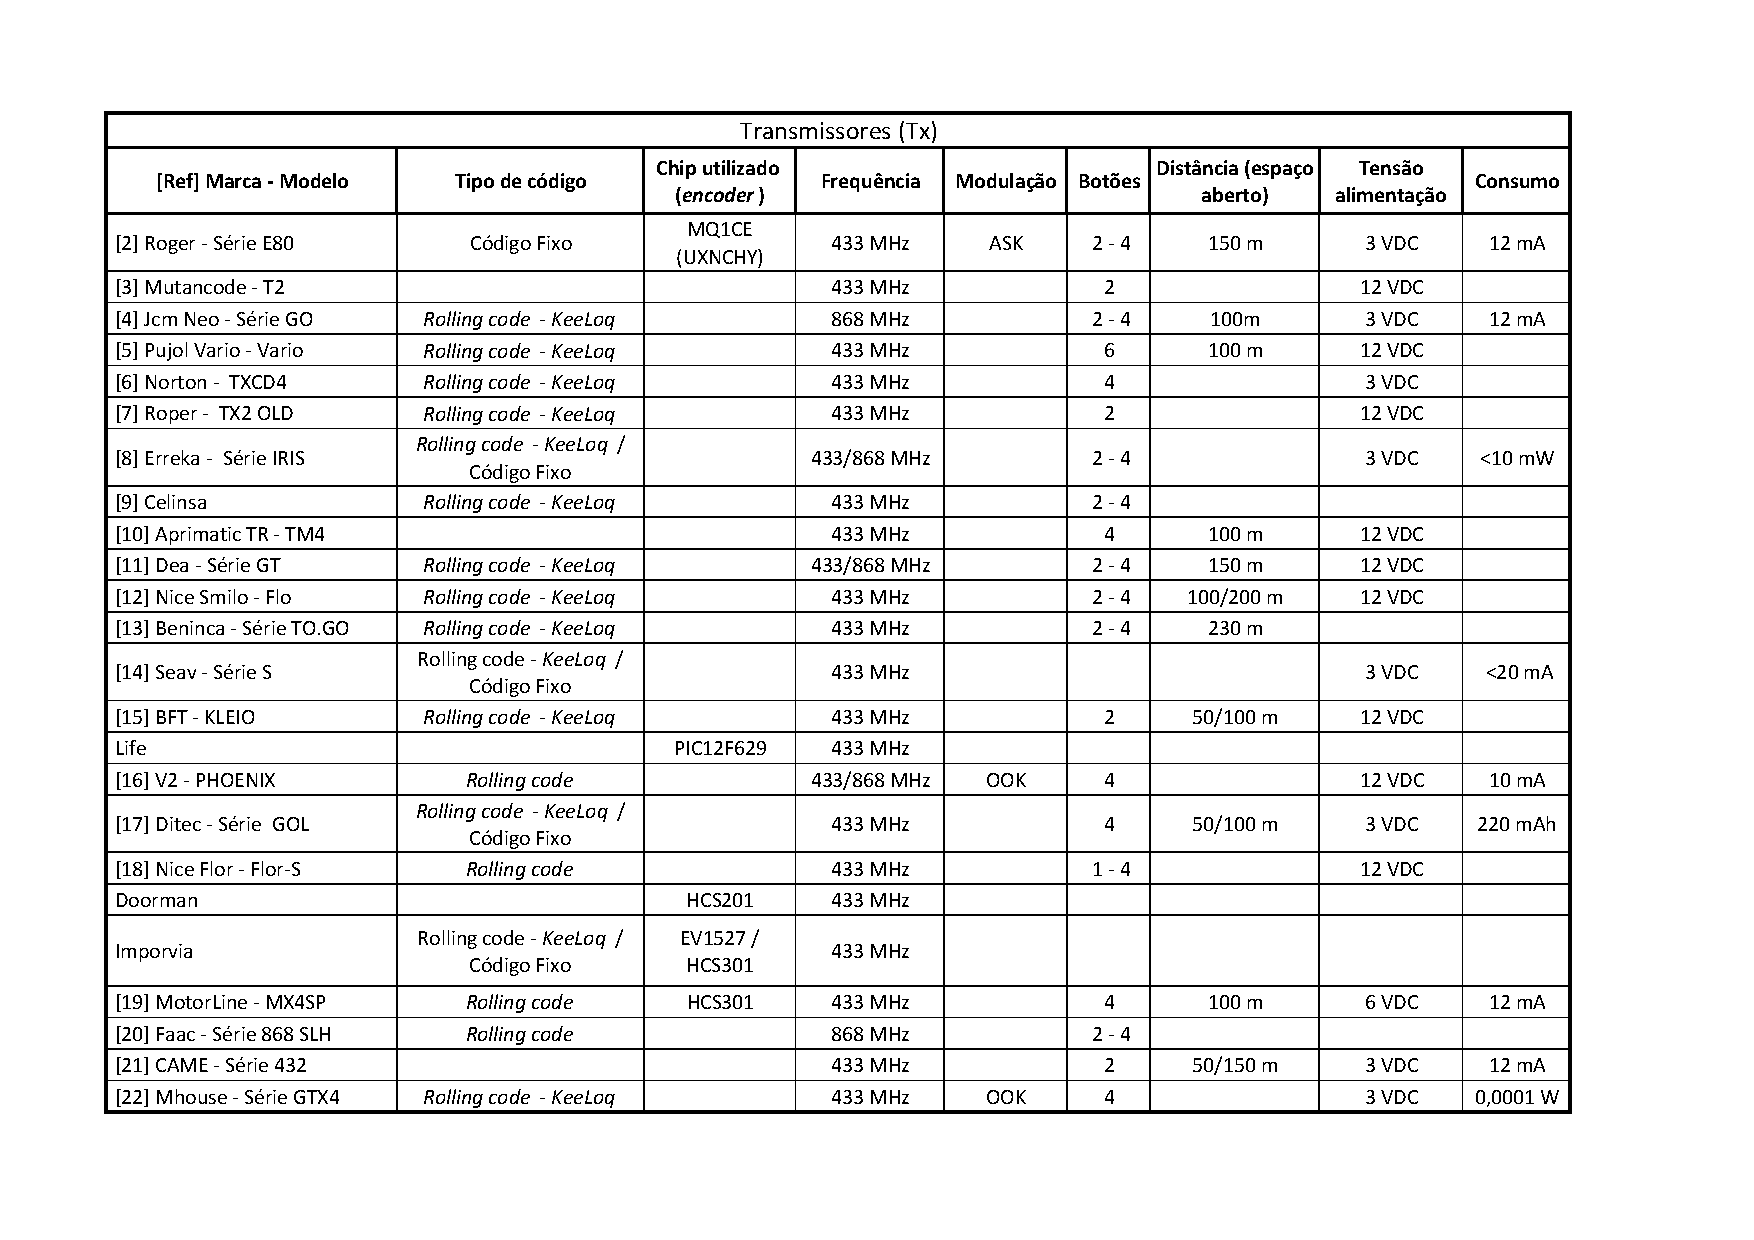
\includegraphics[clip, trim=1.6cm 2cm 3cm 1.7cm, width=1\linewidth]{Figuras/tx}
	\caption{Caracter�sticas de alguns transmissores existentes no mercado.}
	\label{fig:tx}
\end{table}
\begin{figure}[H]
	\centering
	\begin{subfigure}{.33\textwidth}
		\centering
		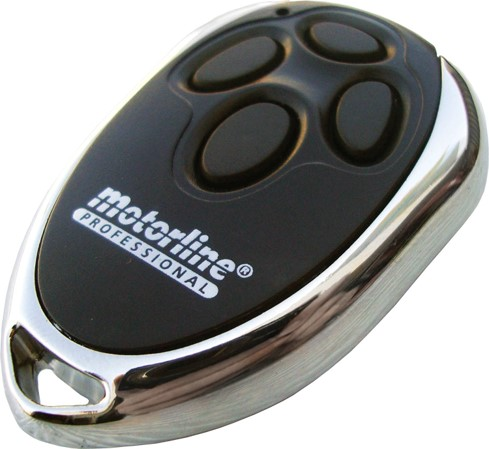
\includegraphics[clip, width=0.5\linewidth]{Figuras/motorline}
		\captionsetup{labelformat=empty}
		\caption{(a) Comando da Motorline [\ref{motorlineremotelink}].}
	\end{subfigure}%
	\begin{subfigure}{.33\textwidth}
		\centering
		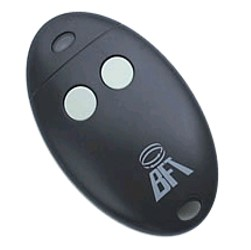
\includegraphics[clip, trim=0cm 0.3cm 0cm 0cm, width=0.48\linewidth]{Figuras/bft}
		\captionsetup{labelformat=empty}
		\caption{(b) Comando da BFT [\ref{bftremotelink}].}
	\end{subfigure}
	\begin{subfigure}{.33\textwidth}
		\centering
		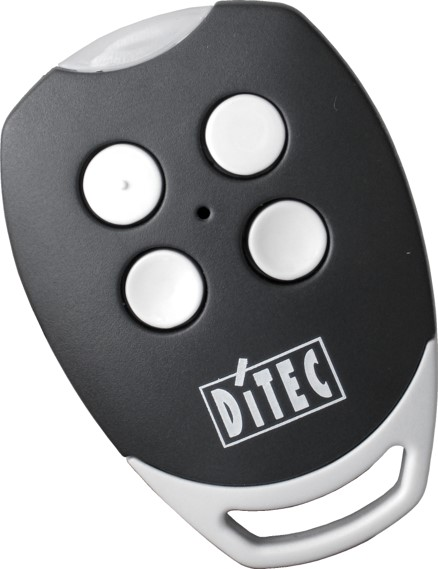
\includegraphics[clip, width=0.345\linewidth]{Figuras/ditec}
		\captionsetup{labelformat=empty}
		\caption{(c) Comando da D�tec [\ref{ditecremotelink}].}
	\end{subfigure}
	\caption{Exemplos de comandos remotos existentes no mercado.}
	\label{fig:comandosmarcas}
\end{figure}
\subsection{Unidades recetoras}
No mercado existem dispon�veis bastantes unidades centrais, tal como se pode verificar pelos dados constantes nas tabelas \ref{fig:rx1} e \ref{fig:rx2}. Estas tabelas apresentam as caracter�sticas t�cnicas principais de v�rios recetores comerciais. Como se pode constatar, a frequ�ncia de opera��o e o tipo de codifica��o utilizados nas unidades recetoras est�o de acordo com os dados apresentados para os comandos. A frequ�ncia de opera��o destas unidades � sempre �nica, apesar de poder ser de 433 MHz ou de 868 MHz. Apesar de existirem modelos de determinadas marcas que permitem a opera��o em qualquer uma das duas, � necess�rio optar por uma, porque o circuito externo de adapta��o de imped�ncia � diferente consoante a frequ�ncia. Relativamente aos tipos de codifica��o, existem recetores que apenas permitem a rece��o de c�digos fixos, outros detetam apenas os \textit{rolling codes} e existem ainda os que permitem a rece��o de ambos. A n�vel das modela��es utilizadas pelos recetores, os dados apurados n�o s�o conclusivos. Como se pode verificar, apenas uma das marcas fornece essa informa��o onde refere a utiliza��o de uma modela��o \textit{amplitude-shift keying} (ASK).\\[6pt]
� poss�vel observar ainda nas tabelas \ref{fig:rx1} e \ref{fig:rx2}, que o n�mero de canais/sa�das de um recetor, isto �, o n�mero de mecanismos que um recetor consegue acionar, varia de modelo para modelo, sendo tipicamente de 2 a 4. O n�mero de comandos que cada recetor � capaz de memorizar tamb�m � vari�vel, existindo modelos que guardam centenas utilizadores e outros t�m a capacidade de suportar at� milhares de utilizadores. A opera��o de guardar em mem�ria estes comandos/utilizadores, bem como a escolha do tipo de codifica��o reconhecida (nos recetores onde � necess�ria a escolha), � feita por bot�o de press�o ou por DIP \textit{switch}.\\[6pt]
O tipo de comunica��o sem fios utilizado por cada modelo est� tamb�m indicado nas tabelas \ref{fig:rx1} e \ref{fig:rx2}. Como se pode verificar, existem modelos onde a comunica��o � feita numa das bandas ISM (433 MHz ou 868 MHz), enquanto noutros � utilizada a banda dedicada ao GSM (900 MHz). � importante referir que n�o foram encontrados modelos que utilizem ambas as bandas ou ambos os m�todos de comunica��o.\\[6pt]
Numa perspetiva mais t�cnica, ainda s�o poss�veis observar dados como o consumo e a gama de temperatura de opera��o. Como se pode ver, a maioria dos recetores funcionam com alimenta��es de 12 V/24 V AC/DC, existindo, no entanto, alguns que s�o alimentados diretamente a partir da rede el�trica (230 V).
\begin{table}[H]
	\centering
	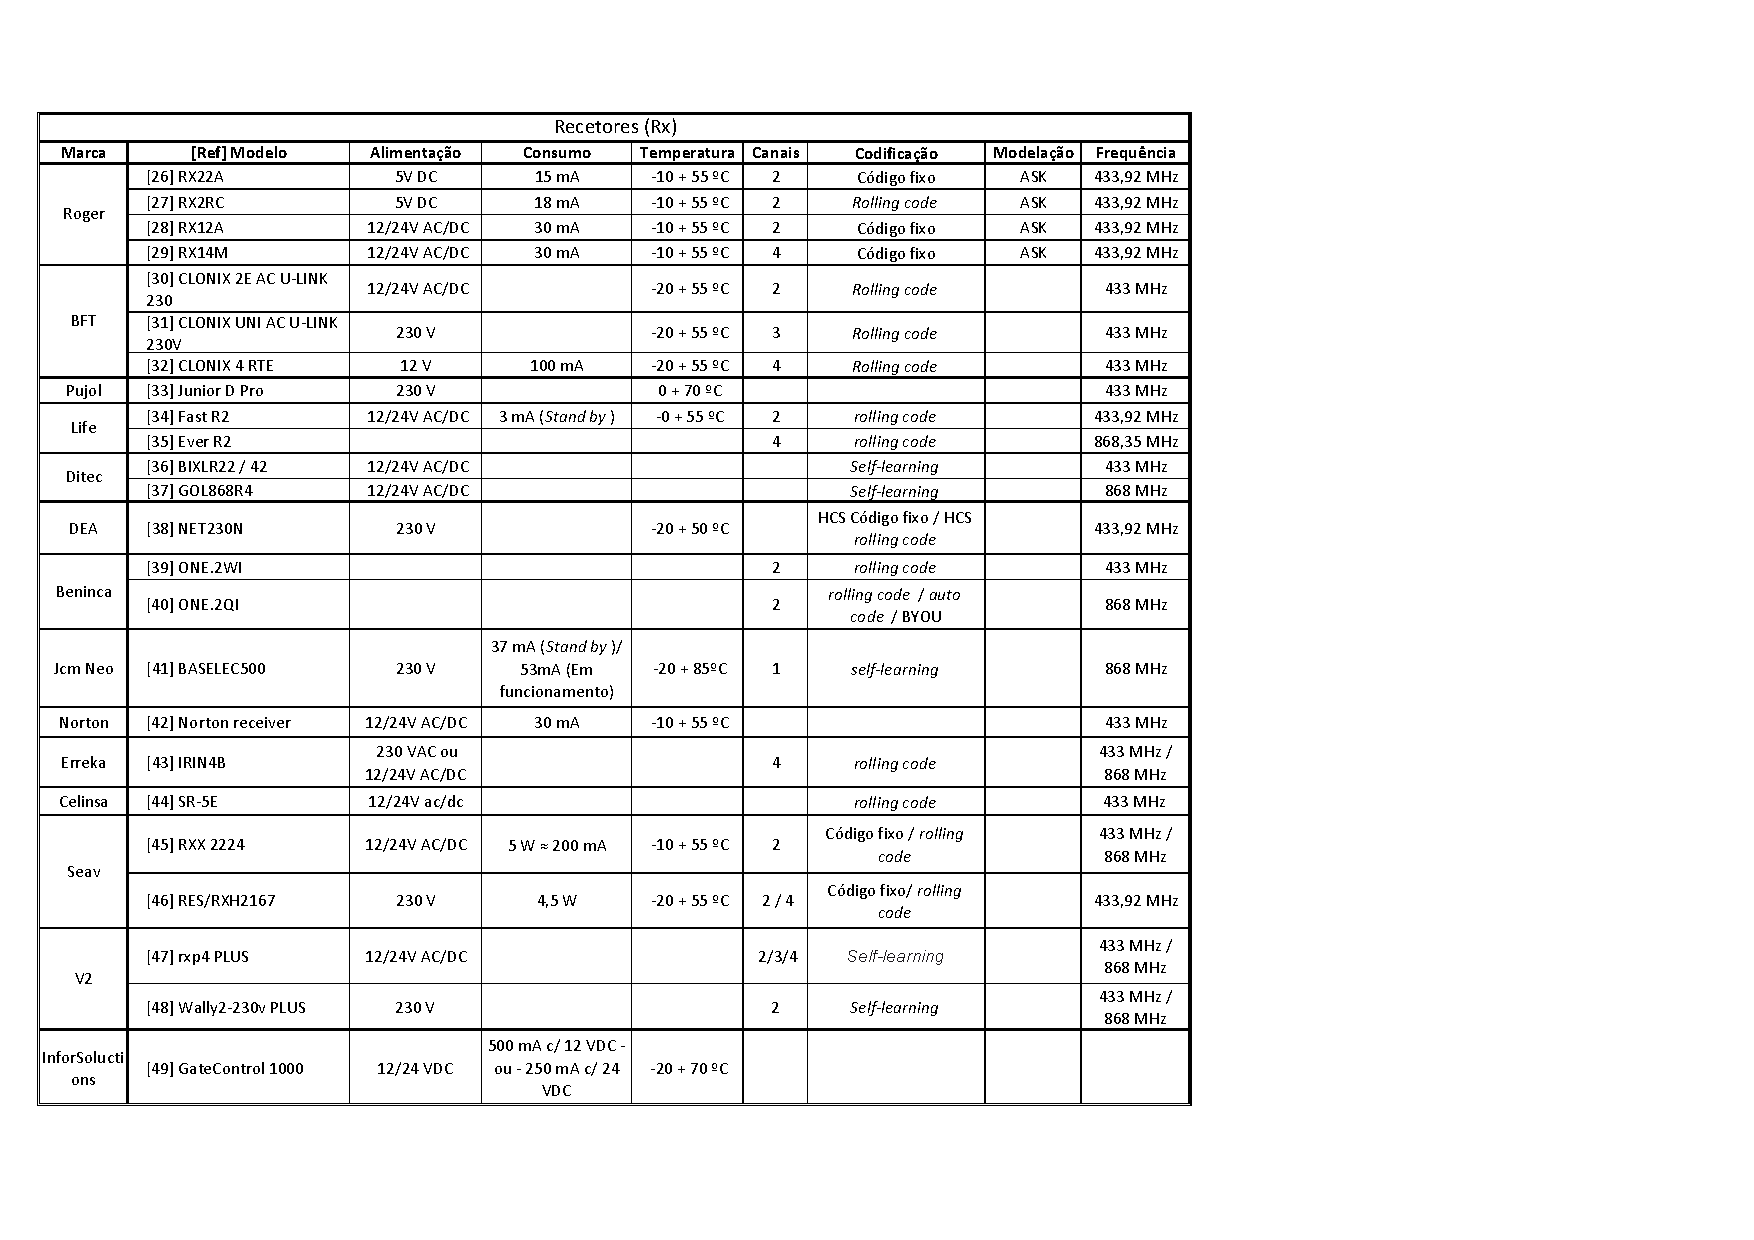
\includegraphics[clip, trim=0.6cm 2.2cm 9.5cm 1.8cm, width=0.98\linewidth]{Figuras/rx1}
	\caption{Caracter�sticas de alguns recetores existentes no mercado.}
	\label{fig:rx1}
\end{table}\vfill\pagebreak
\begin{table}[H]
	\centering
	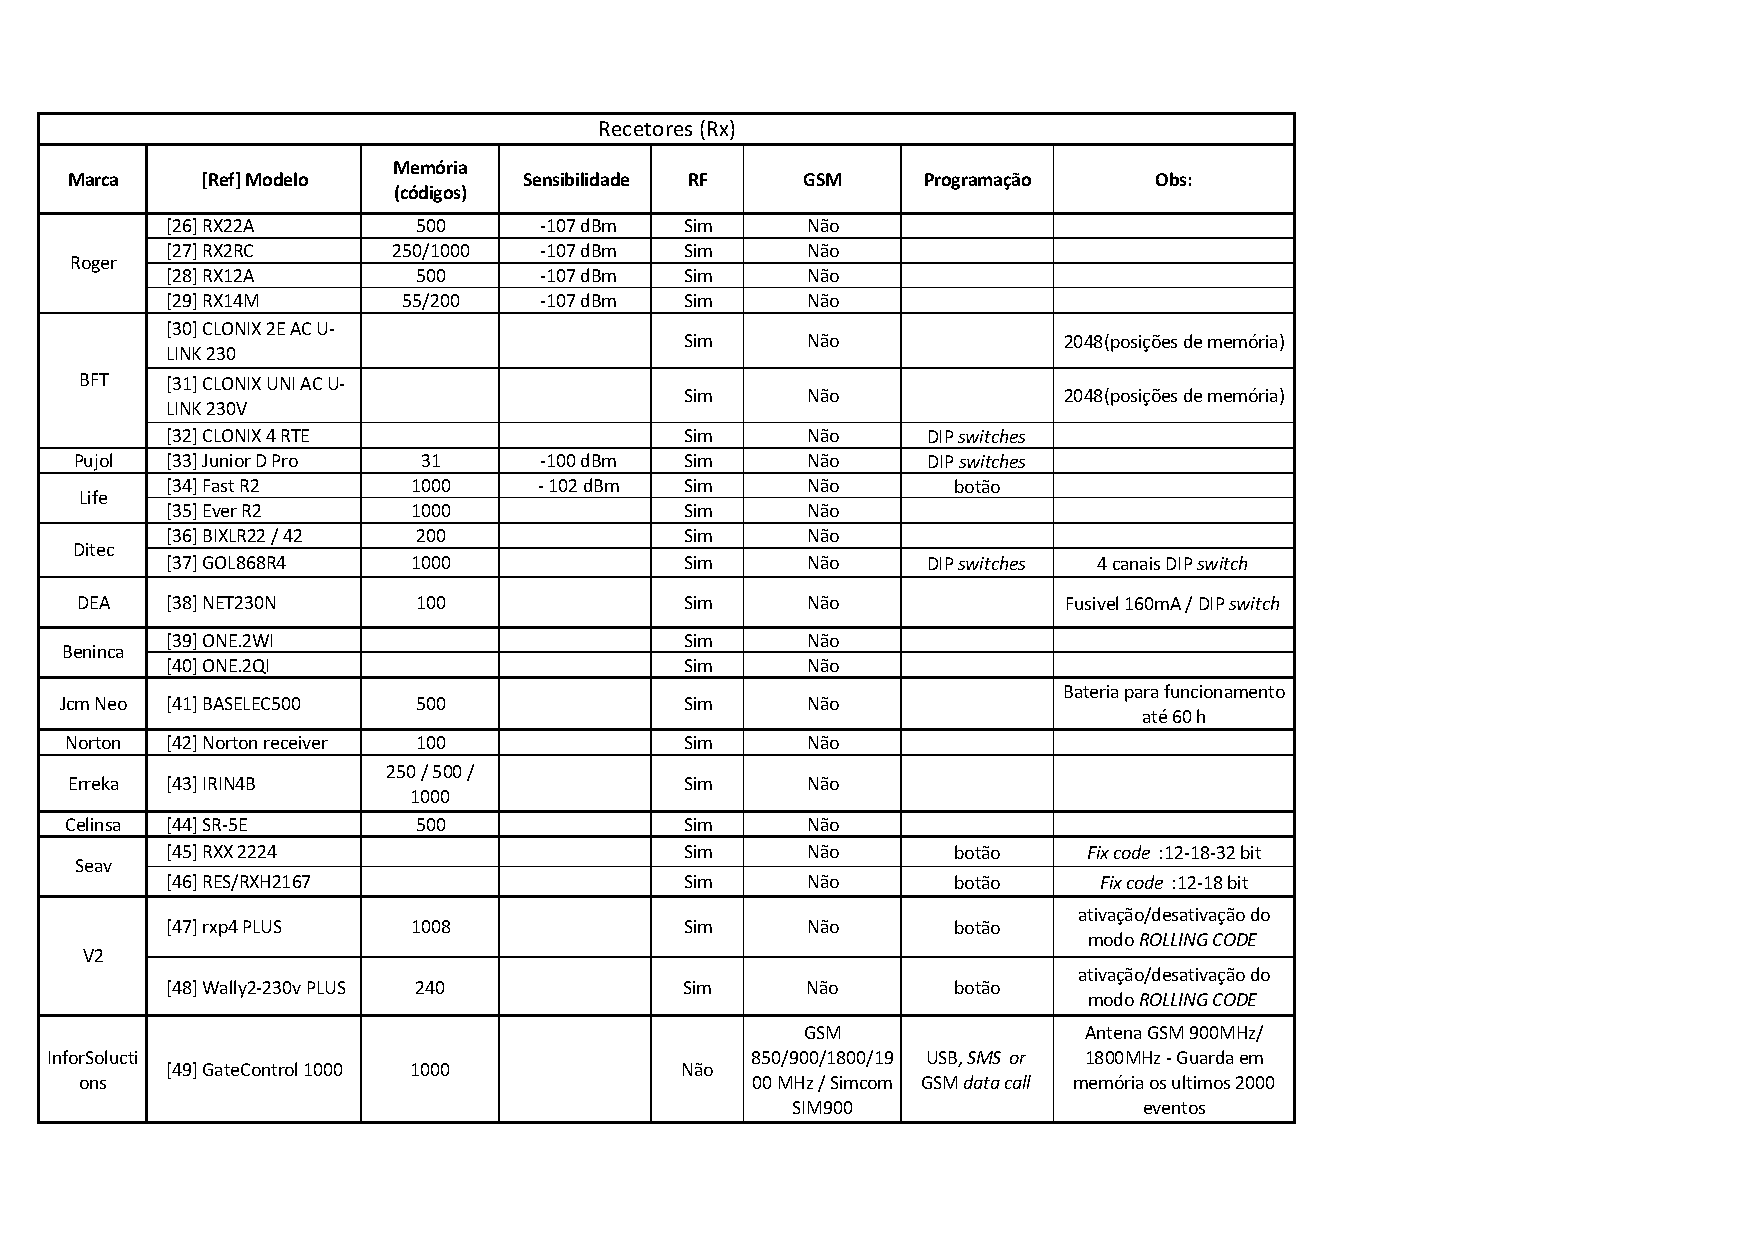
\includegraphics[clip, trim=0.4cm 2cm 7.7cm 1.8cm, width=1\linewidth]{Figuras/rx2}
	\caption{Continua��o das caracter�sticas dos recetores.}
	\label{fig:rx2}
\end{table}
Os consumos destas unidades s�o vari�veis de modelo para modelo, tipicamente abaixo dos 100 mA, contudo � de salientar que nestes apenas h� exist�ncia de um m�dulo r�dio para a rece��o de comandos, onde o seu consumo � baixo, e tamb�m n�o h� informa��es sobre o estado de funcionamento, isto �, em que condi��es � que os recetores apresentam estes consumos (e.g., estado das sa�das). Relativamente �s temperatura de opera��o, estes recetores est�o preparados para funcionarem numa gama de temperaturas compreendidas entre os -20 �C at� aos 55 �C (tipicamente), suportando assim uma vasta gama de temperaturas ambiente. Existe ainda um modelo que permite o funcionamento da unidade recetora alimentado a bateria durante 60 h, no caso de falha de alimenta��o externa.\\[6pt]
Na figura \ref{fig:recetoressmarcas} s�o apresentados alguns dos recetores existentes no mercado.
\begin{figure}[H]
	\centering
	\begin{subfigure}{.36\textwidth}
		\centering
		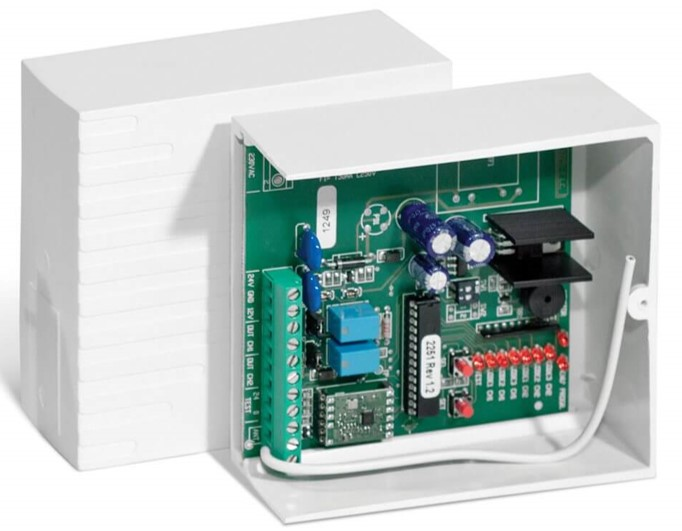
\includegraphics[clip, width=0.7\linewidth]{Figuras/motorlinereceiver}
		\captionsetup{labelformat=empty}
		\caption{(a) Recetor da Motorline [\ref{motorlinereceiverlink}].}
		\label{fig:motorlinereceiver}
	\end{subfigure}%
	\begin{subfigure}{.36\textwidth}
		\centering
		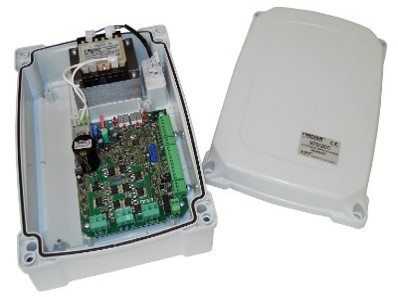
\includegraphics[clip, width=0.74\linewidth]{Figuras/rogerreceiver}
		\captionsetup{labelformat=empty}
		\caption{(b) Recetor da Roger Technology [\ref{rogerreceiverlink}].}
		\label{fig:rogerreceiver}
	\end{subfigure}
	\begin{subfigure}{.27\textwidth}
		\centering
		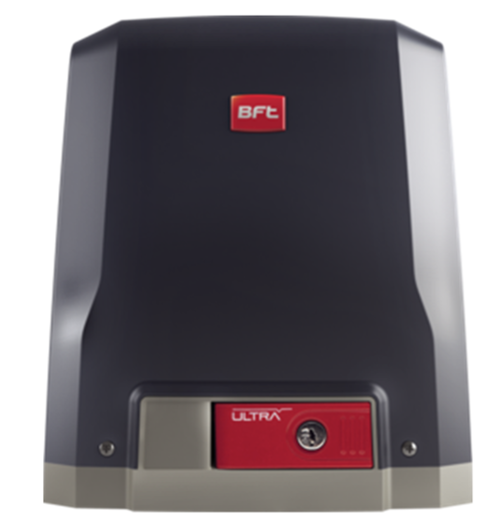
\includegraphics[clip, width=0.695\linewidth]{Figuras/bftreceiver}
		\captionsetup{labelformat=empty}
		\caption{(c) Recetor da BFT [\ref{bftreceiverlink}].}
		\label{fig:bftreceiver}
	\end{subfigure}
	\caption{Exemplos de recetores existentes no mercado.}
	\label{fig:recetoressmarcas}
\end{figure}\vfill\pagebreak
\section{S�mbolos, tramas e c�digos}
A comunica��o entre o comando (unidade transmissora) e o recetor (unidade de controlo e comando) � essencial para o correto funcionamento do sistema de controlo e comando de automatismos. Como referido na sec��o anterior, a modela��o utilizada para a transmiss�o de dados n�o foi conclusiva, contudo na pr�tica foi poss�vel observar, atrav�s de um analisador espetral, que tipicamente se trata de uma modela��o \textit{on-off keying} (OOK). Antes da transmiss�o ser efetuada, os dados a transmitir (sinal em banda base) pelo comando s�o codificados e encapsulados numa trama digital atrav�s de um codificador (\textit{encoder}). Esta trama modula em OOK, � recuperada pelo recetor ap�s a desmodula��o do sinal. Nesta sec��o s�o apresentados os s�mbolos, os diversos campos que comp�em as tramas e os tipos de c�digos utilizados nos comandos remotos.
\subsection{C�digos de linha}
A grande maioria dos comandos dispon�veis no mercado utiliza uma das codifica��es de linha apresentadas na figura \ref{fig:tempocodificacoestab}. Para ambos os tipos de codifica��o, o tempo de bit � dividido em tr�s intervalos de tempo iguais. A informa��o digital (``0s'' ou ``1'') a transmitir est� na sua ess�ncia contida no intervalo de tempo central. Os restantes dois intervalos temporais servem para introduzir redund�ncia para dete��o e poss�vel corre��o de erros. Na codifica��o A tem-se sempre o valor l�gico alto no primeiro intervalo de tempo e zero no �ltimo. J� na codifica��o B, verifica-se exatamente o contr�rio.
Estes tipos de c�digos garantem um conte�do espectral reduzido em baixa frequ�ncia (em torno de 0 Hz) e duas transi��es (flancos ascendentes ou descendentes) por cada s�mbolo mesmo quando se transmitem longas sequ�ncias de ``0s'' ou ``1s''. Devido ao elevado n�mero de transi��es, as sincroniza��es de portadora, de trama e de s�mbolo que t�m de ser efetuadas no recetor s�o facilitadas.
Apesar das codifica��es indicadas na Figura \ref{fig:tempocodificacoestab} serem as mais conhecidas e utilizadas nos sistemas de controlo e comando de automatismos, existem outras, sendo, no entanto, codifica��es propriet�rias. Na figura \ref{fig:codificacoestab} s�o apresentadas as formas de s�mbolo para o valor l�gico '1' e '0' em cada uma das codifica��es.
\subsection{Composi��o das tramas}
Para que a transmiss�o da informa��o possa ser feita de forma eficiente, os dados transmitidos pelos comandos s�o organizados em tramas. Dependendo do fabricante, cada trama pode estar dividida em v�rios blocos.\\[6pt]
Pelos \textit{datasheets} dos \textit{encoders} apresentados na tabela \ref{fig:tx}, foi recolhida a informa��o apresentada na figura \ref{fig:temposimb}. Como � poss�vel observar, existem algumas rela��es (fatores multiplicativos) entre os tempos dos diversos campos existentes na trama. Por exemplo � poss�vel observar que meio per�odo de pre�mbulo, $T_{E}$, � 3 vezes menor que um per�odo de s�mbolo, $T_{BP}$, isto �: $3T_{E}=T_{BP}$. Ainda se pode verificar que o tempo de \textit{header} (parte da trama onde s�o transmitidos zeros), $T_{H}$, � 10 vezes maior que $T_{E}$, ou seja, $T_{H} = 10T_{E}$.
\begin{figure}[H]
	\centering
	\begin{subfigure}{.6\textwidth}
		\centering
		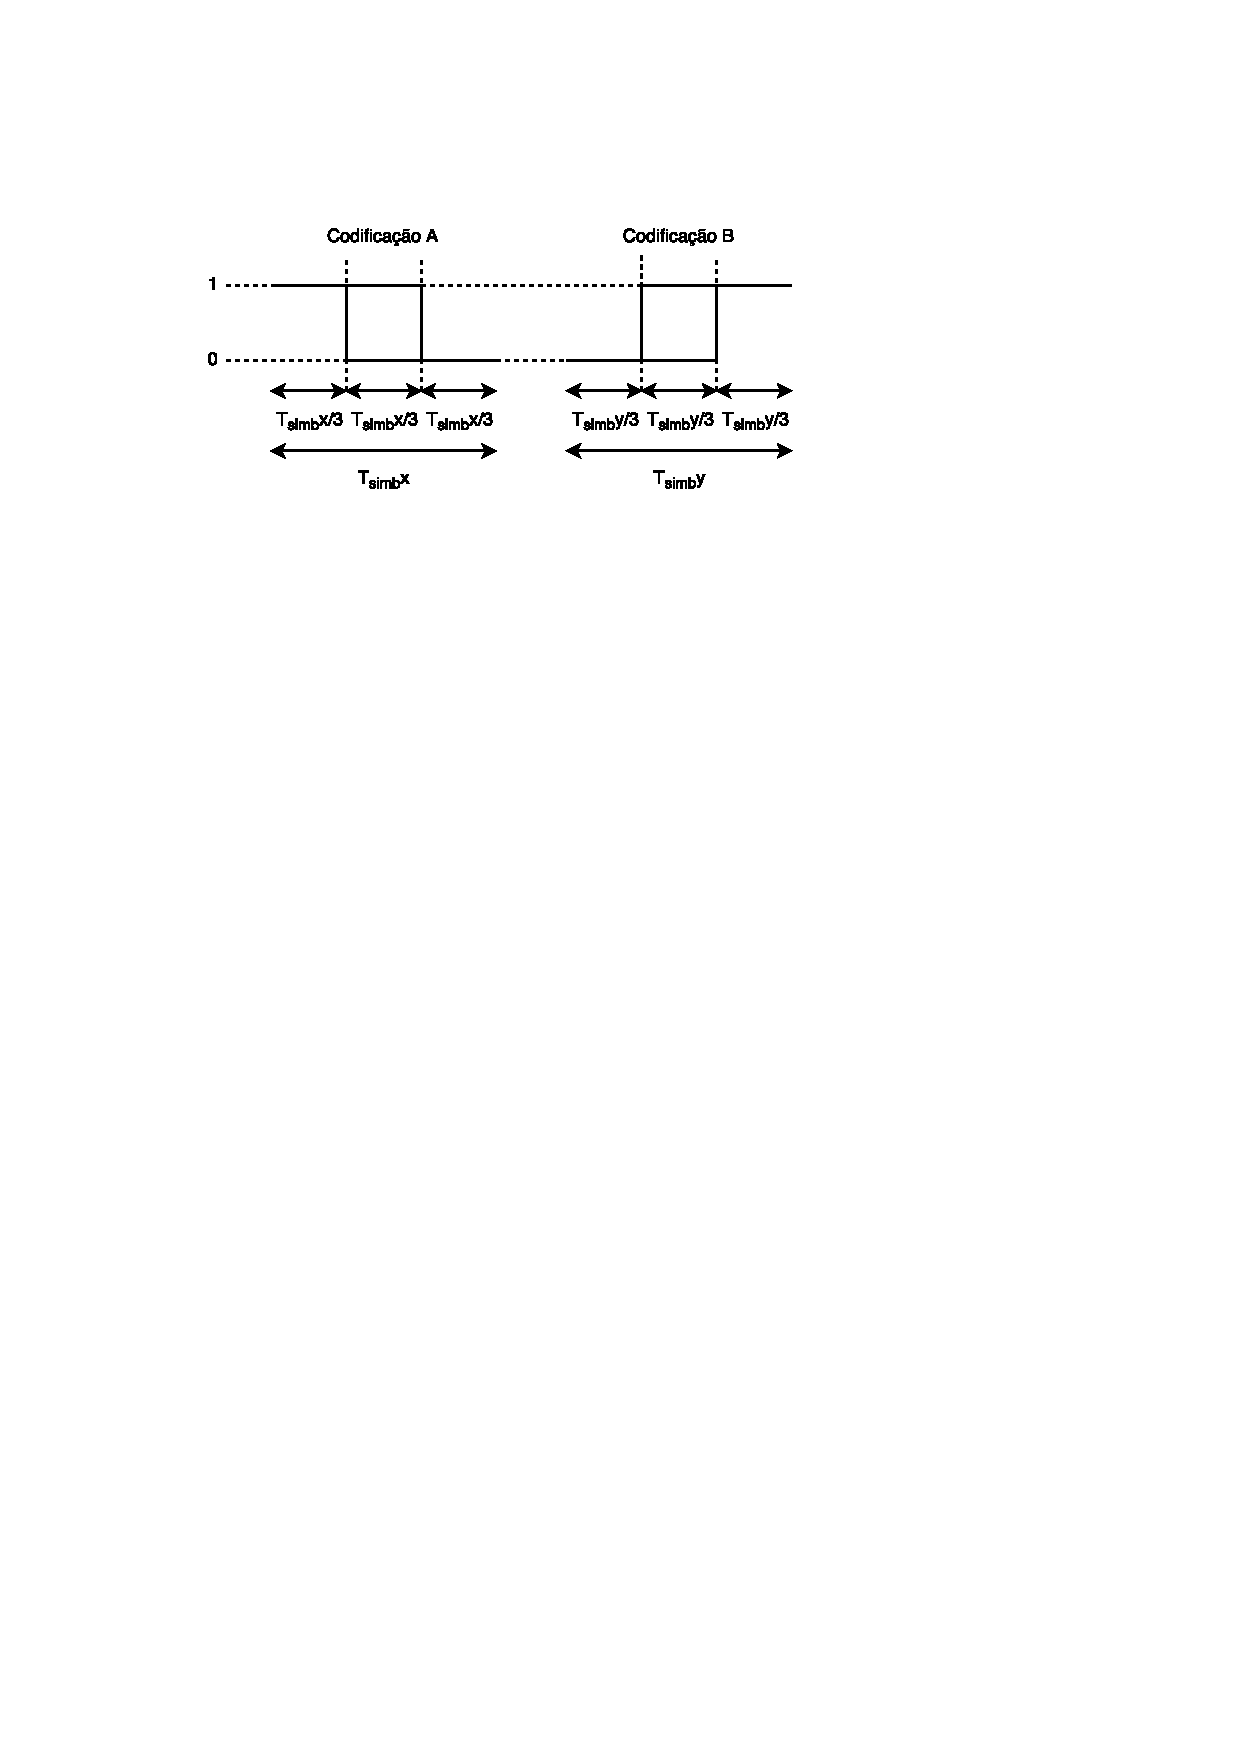
\includegraphics[clip, trim=3.5cm 21.2cm 7.4cm 3.75cm, width=0.81\linewidth]{Figuras/codificacoes}
		\captionsetup{labelformat=empty}
		\caption{(a) Tipos de codifica��es.}
		\label{fig:tempocodificacoestab}
	\end{subfigure}%
	\begin{subfigure}{.4\textwidth}
		\centering
		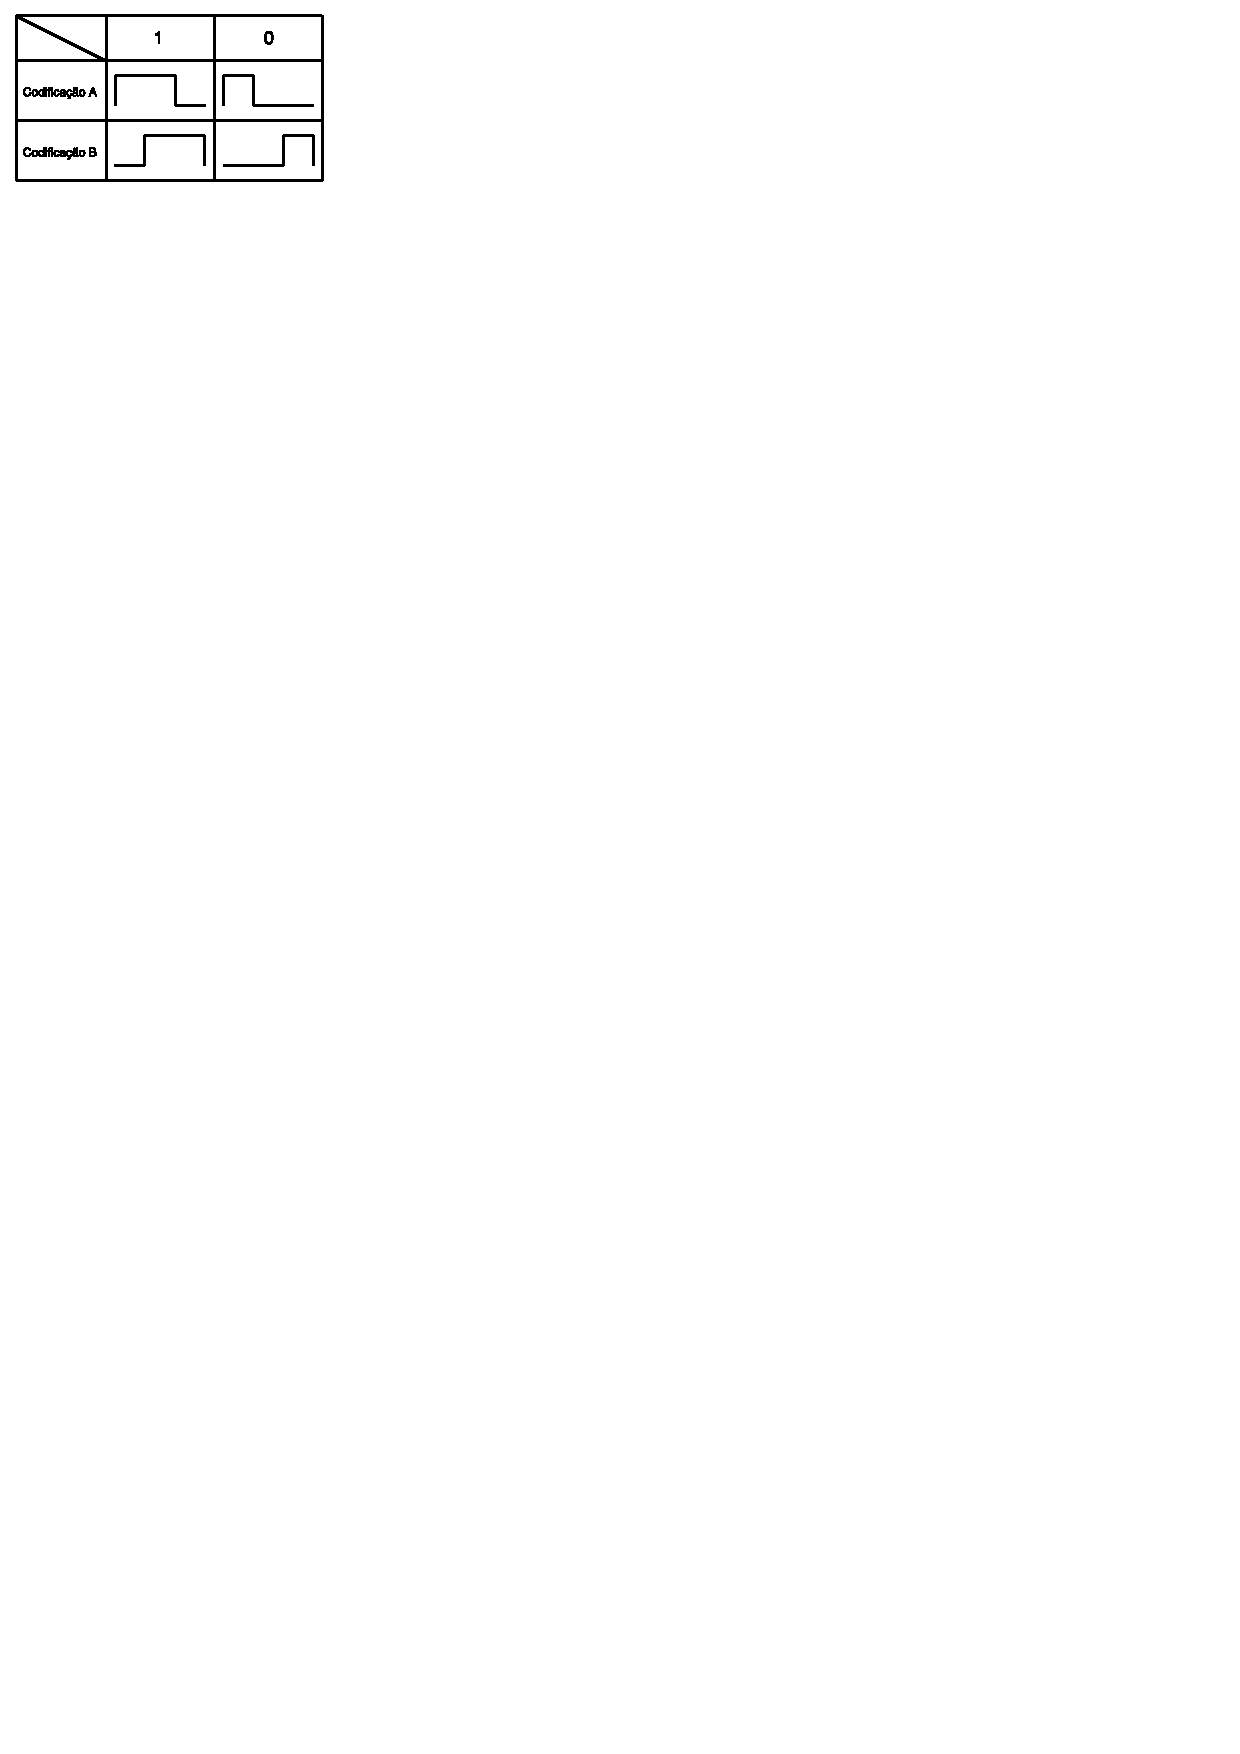
\includegraphics[clip, trim=0cm 26.5cm 15.2cm 0cm, width=1\linewidth]{Figuras/simbolos}
		\captionsetup{labelformat=empty}
		\caption{(b) Tipo de s�mbolos.}
		\label{fig:codificacoestab}
	\end{subfigure}
	\caption{Codifica��es A e B.}
	\label{fig:codificacoes}
\end{figure}

\begin{figure}[H]
	\centering
	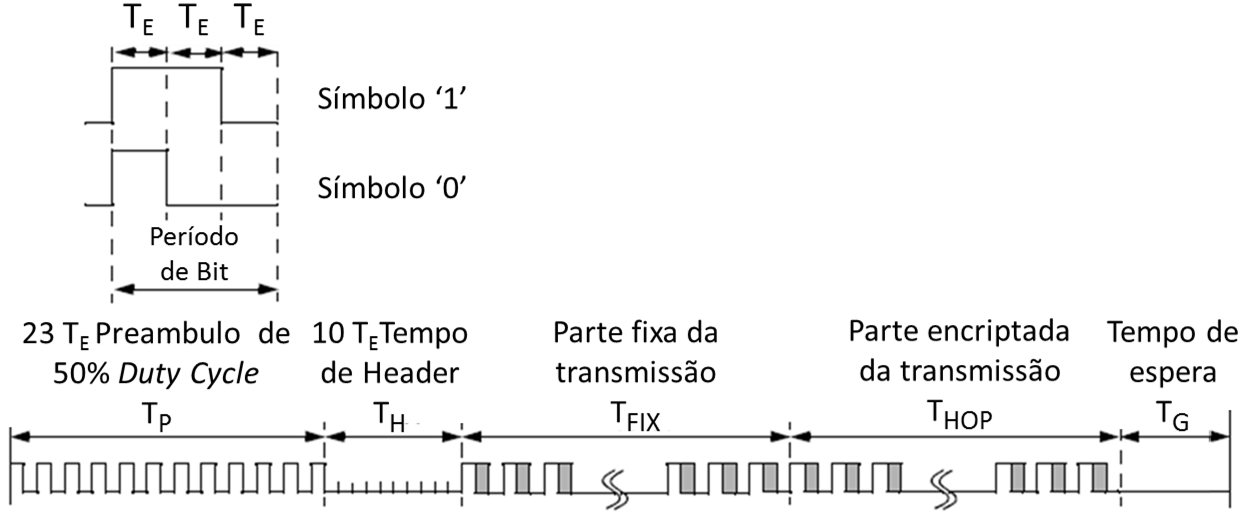
\includegraphics[clip, width=0.75\linewidth]{Figuras/tempoSimb}
	\caption{Tempos de trama [\ref{hcs301}].}
	\label{fig:temposimb}
\end{figure}
Na pr�tica isto apenas se verifica � sa�da do \textit{encoder}. Ap�s a desmodela��o por parte do transcetor estas condi��es deixam de ser verdadeiras. Para al�m disso n�o � garantido que em todos os comandos estas rela��es se verifiquem.\\[6pt]
Nas tramas com mais do que um bloco, o primeiro � sempre um bloco de pre�mbulo. O pre�mbulo � composto por uma sequ�ncia de ``0s'' e ``1s'', ou seja, pode ser visto como um ``peda�o'' do rel�gio (\textit{clock}) utilizado na gera��o dos dados que se pretendem transmitir. A sua dura��o ou tamanho depende do \textit{encoder} utilizado (depende do fabricante). O pre�mbulo � utilizado neste tipo de sistemas para facilitar a captura e gera��o dos v�rios sinais de sincronismo no recetor e assim evitar perdas de informa��o durante a comunica��o entre o comando e a unidade de rece��o.\\[6pt]
O transcetor ao receber os dados modelados em OOK vindos de um comando � frequ�ncia de 433 MHz (com possibilidade de deslocamento da frequ�ncia na ordem dos kilohertz), tem como objetivo colocar esse sinal em banda base (BB) ou numa frequ�ncia interm�dia (IF), isto �, realizar a sua desmodela��o ou deslocar o sinal na frequ�ncia, respetivamente. Para isso � utilizada uma malha de captura de fase (PLL), um cristal e um misturador (\textit{mixer}). Enquanto o sinal de sa�da do misturador n�o estiver na frequ�ncia desejava, a PLL vai sofrer ajustes, pelo controlo autom�tico de frequ�ncia (AFC) at� a obter (tempo de bloqueio). Como o pre�mbulo � caracterizado por ter elevado n�mero de comuta��es e como a desmodela��o � feita por dete��o s�ncrona (sem detetor de envolvente), este � utilizado neste tipo de sistemas para o sincronismo do recetor. O pre�mbulo � o primeiro bloco da trama a ser transmitido e assim servir� para a fixa��o da PLL. Como este � caracterizado, neste caso, por apenas conter informa��o temporal, isto �, rela��es temporais entre os v�rios elementos que comp�em a trama, n�o � cr�tico que enquanto a PLL n�o estiver bloqueada, sejam perdidos alguns per�odos da onda, pois estes v�o repetir-se v�rias vezes. No fim da rece��o deste bloco, ao come�ar a receber o pr�ximo (bloco de dados), a PLL j� se encontra bloqueada, o que se traduz numa rece��o total e sem perdas de informa��o.
\subsection{C�digos}
Na pesquisa efetuada, tanto das unidades transmissoras como das recetoras, foi poss�vel observar a exist�ncia de 3 tipos de c�digo: o c�digo fixo, o \textit{rolling code} que utiliza o algoritmo \textit{KeeLoq} e o \textit{rolling code} que n�o utiliza esse algoritmo. Apesar de todos eles terem em comum a possibilidade de exist�ncia de pre�mbulo, possu�rem bits de identifica��o do bot�o/canal e ainda possu�rem o n�mero de s�rie do comando, os c�digos t�m diferen�as nas tramas geradas pelos \textit{encoders}, tanto na sua organiza��o como na sua composi��o.
\subsubsection{C�digo fixo}
O c�digo fixo � um dos tipos de c�digo utilizado nos comandos e recetores de sistemas de controlo remoto de automatismos. Estes podem conter um ou dois bloco de trama, isto �, podem possuir pre�mbulo ou n�o. Para al�m disso s�o caracterizados pela exist�ncia de apenas 4 bits identificadores de sa�da/canal e um n�mero de identifica��o �nico do comando, n�mero de s�rie. O EV1527 [\ref{ev1527}], apresentado na figura \ref{fig:ev1527}, � um exemplo de codificador deste tipo de trama. Como forma de impedir a clonagem do comando ou o seu uso indevido, existem comandos com a possibilidade de escolha do c�digo transmitido atrav�s de pequenos interruptores (DIP \textit{switches}), tal como se pode ver na figura \ref{fig:dipswitchremote}. Estes funcionam como um cadeado de segredo, isto �, os utilizadores t�m a possibilidade de utilizar o c�digo correto para o acionamento do mecanismo e escolher um c�digo incorreto quando n�o for necess�rio a sua utiliza��o.
\subsubsection{\textit{Rolling code}}
O \textit{rolling code} � outro tipo de c�digo utilizado nos referidos sistemas. Este tipo de c�digo foi criado para aumentar a sua seguran�a e impossibilitar a c�pia do c�digo associado a cada comando. Este tipo de a��o, conhecida como clonagem ou \textit{replay attack}, pode ser efetuada facilmente se a codifica��o utilizada for a fixa. Como os \textit{encoders} destes comandos nunca geram o mesmo c�digo sequencialmente, o c�digo apesar de poder ser copiado, acaba por n�o ser aceite pela unidade central pois j� o recebeu anteriormente. A trama gerada por um \textit{encoder} que utiliza a codifica��o \textit{rolling code} est� ilustrada na figura \ref{fig:rolling}.\\[6pt]
Como se pode verificar, o segundo bloco da trama � composto por uma parte fixa, de 34 bits, e por uma parte encriptada, de 32 bits. Na parte fixa da trama, existe um bit (\textit{Repeat}), que indica que a trama est� a ser repetida pelo mesmo comando e n�o por outro, isto �, como acima referido o \textit{encoder} nunca gera o mesmo c�digo sequencialmente, contudo a trama s� muda quando o bot�o for pressionado novamente, assim para que o recetor saiba que a trama repetida est� a ser enviada pelo mesmo comando e n�o por um outro (clonagem), este bit fica a '1' enquanto o bot�o do comando estiver pressionado. Caso seja efetivamente uma colagem, a primeira trama gerada por esse, enviar� '0' nesse bit e assim o recetor sabe que n�o pode acionar o mecanismo.
\begin{figure}[H]
	\centering
	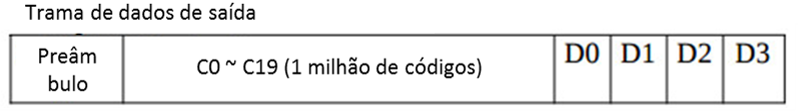
\includegraphics[width=0.55\linewidth]{Figuras/EV1527}
	\caption{Trama gerada pelo \textit{encoder} EV1527 [\ref{ev1527}].}
	\label{fig:ev1527}
\end{figure}
\begin{figure}[H]
	\centering
	\begin{subfigure}{.5\textwidth}
		\centering
		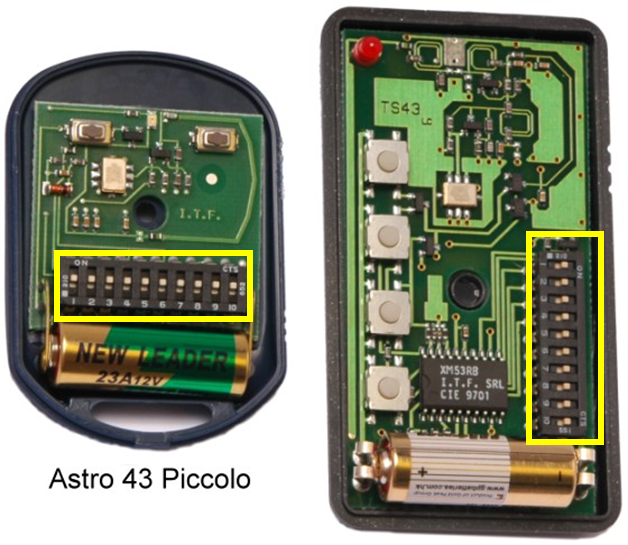
\includegraphics[clip, trim=0cm 2.4cm 9cm 1.2cm, width=0.29\linewidth]{Figuras/comandodip}
		\captionsetup{labelformat=empty}
		\caption{(a) Astro 43 \textit{type} P43/2T.}
	\end{subfigure}%
	\begin{subfigure}{.5\textwidth}
		\centering
		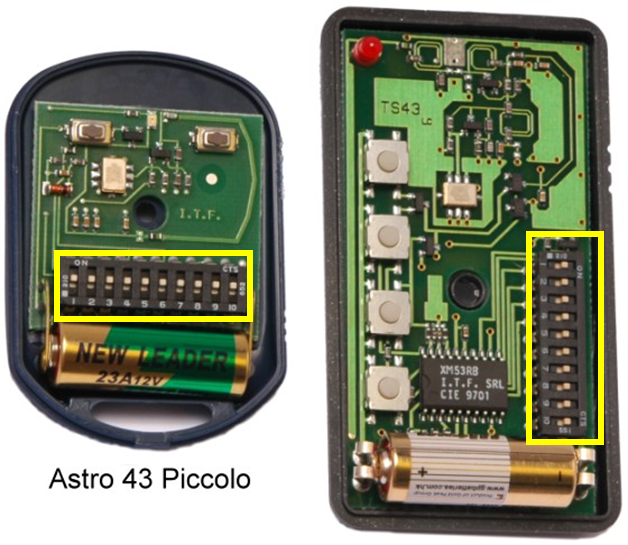
\includegraphics[clip, trim=8.5cm 0cm 0cm 0cm, width=0.225\linewidth]{Figuras/comandodip}
		\captionsetup{labelformat=empty}
		\caption{(b) Astro 43 \textit{type} 43/2T.}
	\end{subfigure}
	\caption{Exemplos de comandos remotos program�veis por DIP \textit{switch} [\ref{dipremote}].}
	\label{fig:dipswitchremote}
\end{figure}
\begin{figure}[H]
	\centering
	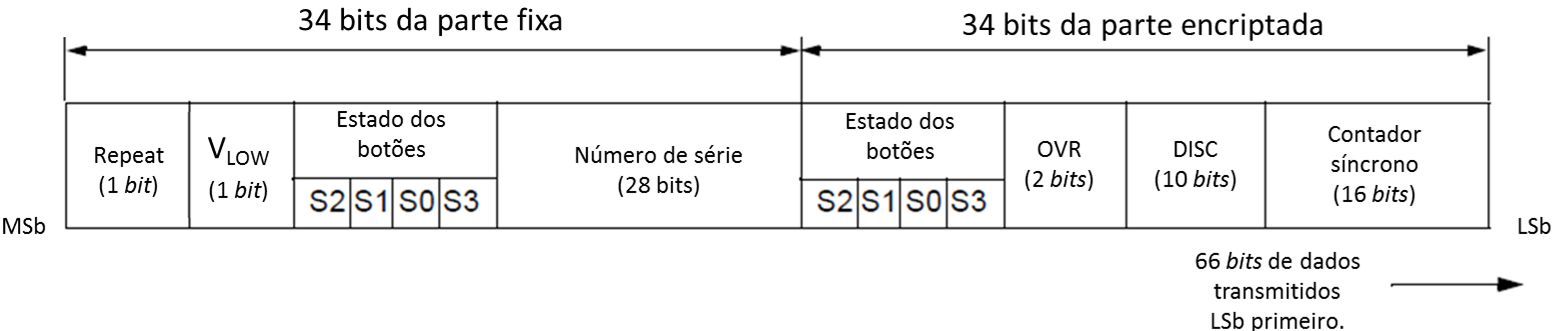
\includegraphics[clip, width=0.85\linewidth]{Figuras/rolling}
	\caption{Constitui��o de uma trama \textit{rolling code} [\ref{hcs301}].}
	\label{fig:rolling}
\end{figure}
\begin{table}[H]
	\centering
	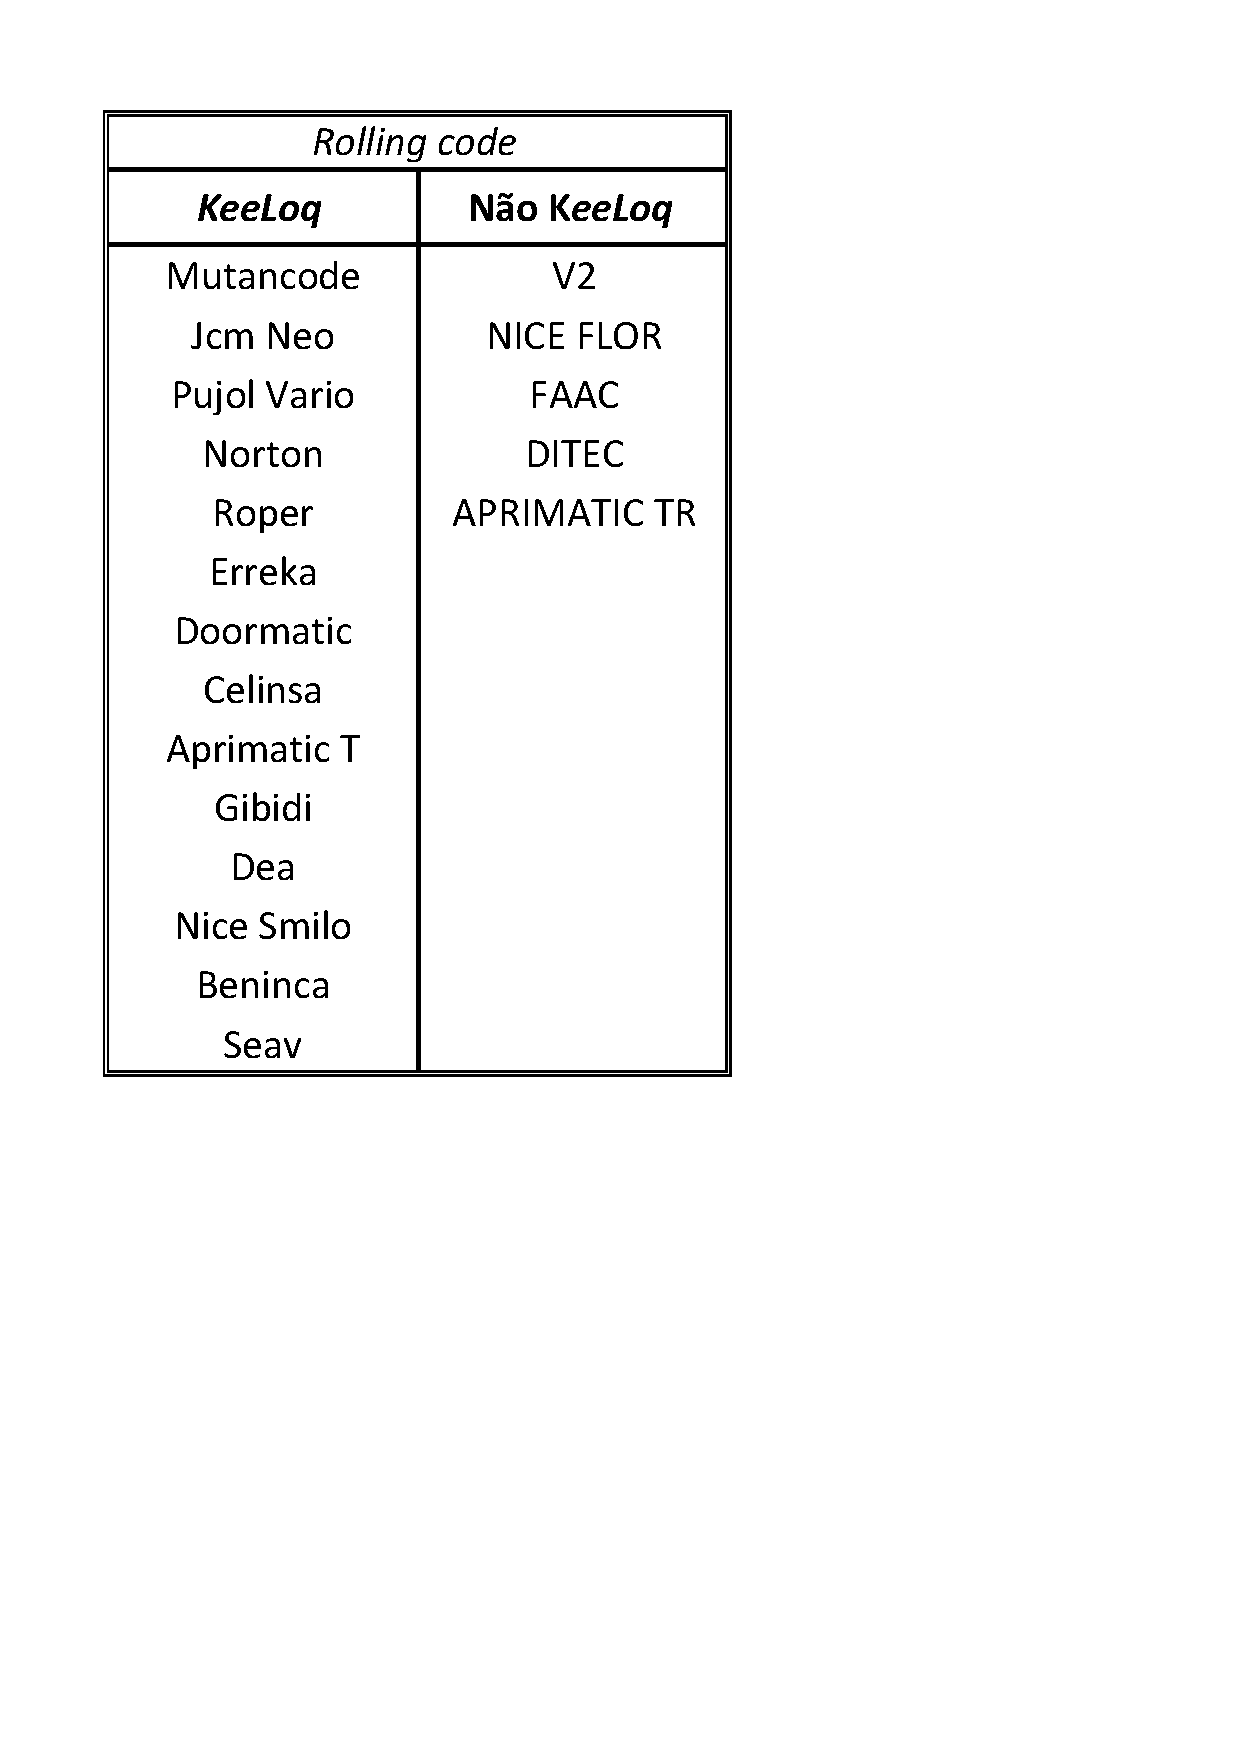
\includegraphics[clip, trim=1.2cm 11.4cm 8.5cm 1.9cm, width=0.27\linewidth]{Figuras/jma}
	\caption{Tipo de \textit{rolling code} implementado pelos diversos fabricantes [\ref{jmalink}].}
	\label{fig:jma}
\end{table}
Pode ainda ver-se que existe um bit (\textit{$V_{LOW}$}) que indica se a bateria do comando est� fraca e existem ainda 4 bits que permitem identificar qual o bot�o que est� a ser pressionado para que a unidade central de controlo saiba qual a sa�da que deve ativar. Os restantes 28 bits da parte fixa correspondem ao n�mero de s�rie do comando, que � um n�mero identificador �nico.\\[6pt]
Um dos tipos de \textit{rolling code} mais utilizado � o \textit{KeeLoq}, tal como se pode observar pela tabela \ref{fig:jma}. Os c�digos que n�o s�o do tipo \textit{KeeLoq} s�o usualmente codifica��es desenvolvidas e implementadas por marcas espec�ficas (codifica��es propriet�rias), sendo por isso uma minoria. O algoritmo \textit{KeeLoq}, est� presente em \textit{encoders} da Microchip, como � caso das s�ries HCS3XX e HCS2XX (e.g., HCS301 [\ref{hcs301}]).
\section{Arquitetura do sistema}
Antes do projeto e implementa��o de um dado sistema eletr�nico � imperativo definir a topologia ou arquitetura do sistema. Para isso, � necess�rio identificar todas as funcionalidades pretendidas e definir as especifica��es iniciais do sistema. Esta informa��o � crucial para definir o diagrama de blocos do sistema, fazer o projeto dos circuitos eletr�nicos, definir os algoritmos de funcionamento e para desenvolver o respetivo c�digo (\textit{firmware} e \textit{software}).
\subsection{Funcionalidades e especifica��es iniciais}
As caracter�sticas t�cnicas e os modos de funcionamento dos sistemas comerciais existentes e o tipo e forma dos dados que s�o utilizados pelos comandos e recetores apresentados nas sec��es anteriores s�o essenciais para definir as funcionalidades e especifica��es da U3C. Al�m disso, os cen�rios de aplica��o definidos no cap�tulo \ref{introducao} s�o tamb�m essenciais para coligir todas as funcionalidades e definir a arquitetura da U3C. Assim, e atendendo ao exposto, foi definido que:
\begin{itemize}[topsep=5pt,itemsep=-1ex,partopsep=1ex,parsep=1ex]
	\item a U3C pudesse ser utilizada em ambientes/aplica��es residenciais e industriais;
	\item a ordem de comando remota pudesse ser feita de duas formas distintas, via comando remoto (banda ISM 433 MHz, utilizada pela maioria dos comandos existentes no mercado) e via telem�vel/\textit{smartphone} (GSM);
	\item a unidade central de controlo e comando fosse universal, ou seja, fosse compat�vel com os protocolos de comunica��o utilizados pela maioria das marcas existentes no  mercado, onde:
	\begin{itemize}[topsep=1pt,itemsep=-1ex,partopsep=1ex,parsep=1ex]
		\item os algoritmos detet�veis pela unidade fossem o c�digos fixos e os \textit{rolling codes} - \textit{KeeLoq} para que o produto final possa ser competitivo a n�vel do mercado;
		\item as codifica��es detetadas e reconhecidas fossem do tipo A e B (ver figura \ref{fig:codificacoes});
		\item a possibilidade de exist�ncia de pre�mbulo;
		\item o tamanho do pre�mbulo pode ser vari�vel;
		\item o tempo de s�mbolo pode ser vari�vel (\textit{bit rate});
		\item o tempo de \textit{header} pode ser vari�vel (ver figura \ref{fig:temposimb});
		\item o tamanho de trama pode ser vari�vel;
		\item o tempo entre tramas pode ser vari�vel (ver figura \ref{fig:temposimb});
		\item a rela��o entre o per�odo do pre�mbulo e tempo de s�mbolo n�o existe;
		\item a rela��o entre o per�odo do pre�mbulo e tempo de \textit{header} n�o existe.
	\end{itemize}\vspace*{5pt}
	\item o controlo via smartphone fosse feito atrav�s de uma aplica��o \textit{Android};
	\item a U3C ser configur�vel a partir de uma aplica��o \textit{Android} espec�fica (a desenvolver);
	\item existisse uma interface na U3C para a grava��o dos comandos remotos;
	\item na unidade recetora fosse utilizada uma mem�ria \textit{erasable programmable read-only memory} (EEPROM) capaz de armazenar todos os dados necess�rios;	
	\item a U3C tivesse v�rios sinalizadores luminosos e sonoros para configura��o ou indica��o de erros;
	\item a alimenta��o dos circuitos da U3C pudesse ser proveniente de uma fonte externa alternada (de 9 Vrms a 24 Vrms) ou de corrente cont�nua (de 9 V a 30 V);
	\item a unidade recetora possu�sse 4 sa�das a rel� para que possa atuar, de forma isolada, 4 automatismos
	\item U3C tivesse 8 entradas digitais isoladas para aux�lio ao controlo ou para informa��o do estado dos automatismos ligados �s suas sa�das;
	\item a U3C possa funcionar em ambientes com elevado ru�do eletromagn�tico (ambiente industrial), sujeito a vibra��es e impactos;
	\item a unidade central de controlo e comando pudesse ser imediatamente comercializada.
\end{itemize}
Relativamente aos algoritmos detet�veis e implementados pela unidade, fator de decis�o na identifica��o do tipo de algoritmo � o n�mero de bits que comp�em a trama, pois esse n�mero � conhecido no caso dos \textit{rolling code}, 66 bits (ver figura \ref{fig:rolling}). Nos \textit{rolling code} a parte encriptada n�o � utilizada, contudo � guardada em mem�ria para que num futuro desenvolvimento possa ser utilizada como m�todo de acr�scimo de seguran�a e robustez do sistema.\\[6pt]
As especifica��es t�cnicas para a U3C definidas ap�s o levantamento das funcionalidades e caracter�sticas t�cnicas dos sistemas existentes est�o indicadas na tabela \ref{fig:especificacoesu3c}. Como se pode ver e comparar com as carater�sticas dos outros sistemas comerciais (ver tabelas \ref{fig:rx1} e \ref{fig:rx2}), a U3C garante as mesmas funcionalidades e caracter�sticas t�cnicas dos melhores sistemas, disponibilizando ainda o controlo \textit{dual}, ou seja, via comando e via \textit{smartphone}, que nenhum dos outros sistemas garante.
\subsection{Diagrama modular}
Com base no funcionamento descrito anteriormente e nas especifica��es indicadas, foi desenvolvido o diagrama de blocos geral da U3C apresentado na figura \ref{fig:arquitetura}. Neste pode-se observar, de uma forma simplificada, a interliga��o de todos os m�dulos do sistema.
\begin{table}[H]
	\centering
	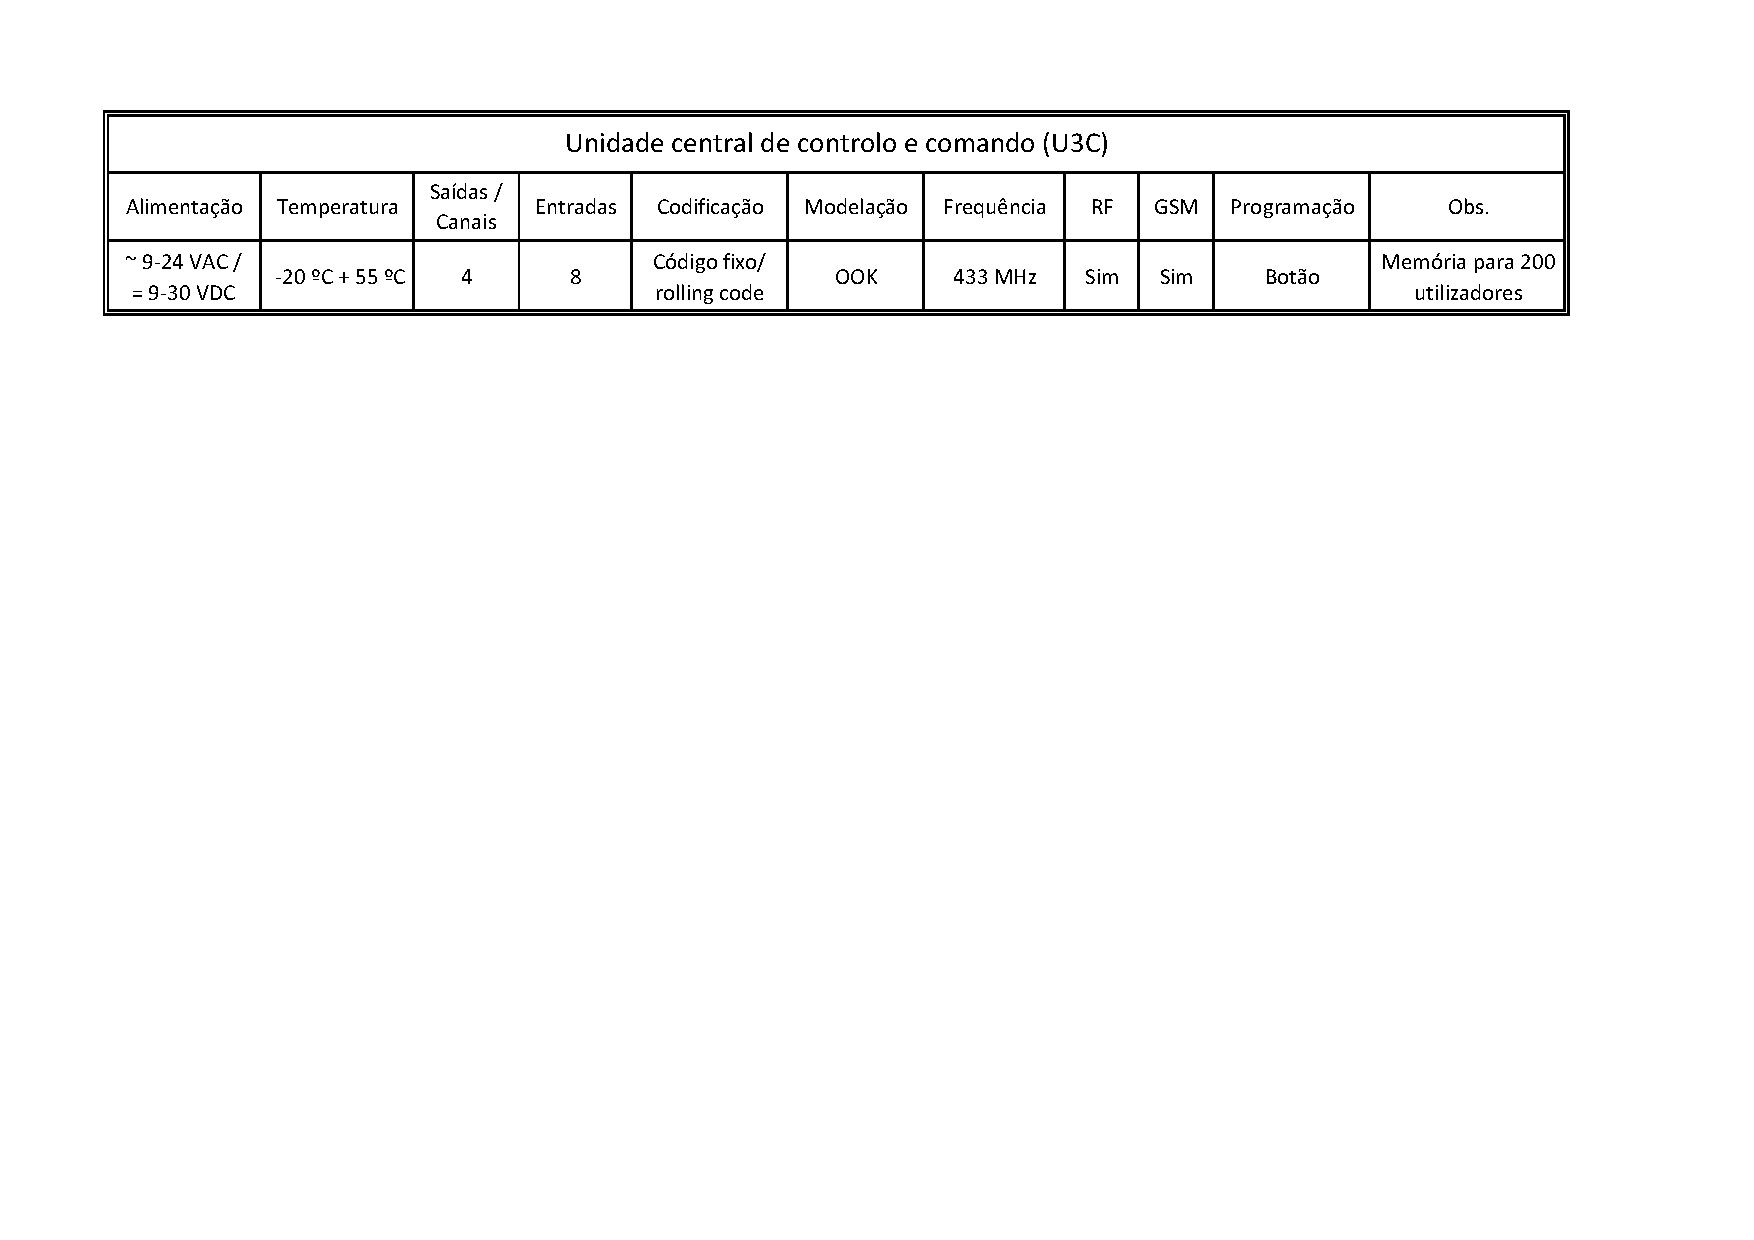
\includegraphics[clip, trim=1.7cm 15.4cm 3.1cm 1.8cm, width=1\linewidth]{Figuras/especificacoesU3Ciniciais}
	\caption{Especifica��es t�cnicas iniciais da U3C.}
	\label{fig:especificacoesu3c}
\end{table}\vfill\pagebreak
\begin{figure}[H]
	\centering
	\includegraphics[clip, trim=4cm 6.8cm 4cm 4.5cm, width=0.68\linewidth]{Figuras/Arquitetura/arquitetura}
	\caption{Diagrama de blocos da arquitetura do sistema.}
	\label{fig:arquitetura}
\end{figure}
\subsubsection{Transmissor}
O transmissor � o comando remoto de radiofrequ�ncia comum que � utilizado na maioria dos sistemas de controlo de automatismos existentes. Estes emitem um c�digo de identifica��o �nico gerado por um \textit{encoder}. Assim, o objetivo � que a U3C seja compat�vel com a maioria dos comandos disponibilizados pelos fabricantes existentes, tais como, Roger, Life, Motorline, Ditec, BFT, DEA, Doorman, entre outros.
\subsubsection{Dispositivo m�vel}
Trata-se de um dispositivo que utiliza um meio de comunica��o GSM para efetuar atua��es e/ou configura��es da unidade central. Incorpora uma interface gr�fica, uma aplica��o \textit{Android}, possibilitando ao utilizador uma intera��o simples e de f�cil utiliza��o. As configura��es poss�veis poder�o ser:
\begin{itemize}[topsep=5pt,itemsep=-1ex,partopsep=1ex,parsep=1ex]
	\item adicionar ou remover utilizadores;
	\item adicionar restri��es a utilizadores;
	\item listar utilizadores adicionados;
	\item aceder a dados relevantes da unidade central;
	\item atuar em sa�das a partir de uma chamada ou \textit{short message service} (SMS).
\end{itemize}
\subsubsection{M�dulo RF}
Trata-se de um m�dulo transcetor que possibilita outra via de comunica��o, a mais vulgar em sistemas de controlo de automatismos existentes. Receber� dados provenientes de comandos remotos, que ao serem desmodulados s�o enviados para o microcontrolador. No fim ser�o tomadas as decis�es apropriadas ao comando recebido. Tamb�m permite o envio de dados por pacotes para a comunica��o entre a U3C e um dispositivo com uma interface RF, tal como descrito anteriormente.
\subsubsection{Mem�ria EEPROM}
M�dulo de mem�ria que armazena todos os dados indispens�veis para o correto funcionamento da unidade central. Neste ser�o guardados dados que dizem respeito aos comandos remotos, tamb�m aos dados dos utilizadores adicionados atrav�s da aplica��o \textit{Android} e ainda aos dados que formam o hist�rico de acessos.
\subsubsection{M�dulo GSM}
Permite a comunica��o via sistema GSM � unidade central, podendo a U3C receber e enviar curtas mensagens de texto e receber chamadas telef�nicas. Este m�dulo recebe de uma forma codificada os comandos de atua��o ou configura��o enviados pelo utilizador, com o aux�lio da aplica��o \textit{Android}.
\subsubsection{Entradas}
As entradas servir�o para a liga��o de dispositivos sensoriais para que a U3C atue, em conformidade, um dado automatismo ou ainda para receber informa��o do estado de funcionamento das sa�das ou dos automatismos ligados �s sa�das. Os sensores que podem ser utilizados s�o sensores comuns, tais como: interruptores, fins-de-curso, fotoc�lulas, entre outros. Os dispositivos sensoriais devem ser passivos, ou seja, apenas de contacto, n�o sendo permitido o uso de sensores que forne�am tens�o ou corrente (sensores ativos). Estas entradas dever�o ter isolamento galv�nico, tanto na fonte que alimenta parte do circuito de entrada, como na interface de liga��o entre as entradas e o microcontrolador. Ter-se-� um conjunto de 8 entradas com o intuito de 2 entradas estarem associadas a uma sa�da.
\subsubsection{Sa�das}
As sa�das s�o a interface da U3C que faz o acionamento direto dos mecanismos que lhe est�o associados. Ser�o disponibilizadas 4 sa�das que ter�o um isolamento galv�nico, utilizando rel�s para esse efeito. Nestas sa�das poder�o ser ligados atuadores, tais como, l�mpadas, controladores de port�es, de cancelas, estores, entre outros sistemas.
\subsubsection{Microcontrolador}
� respons�vel por todo o processamento de dados e comandos da U3C, sendo por isso a interface entre todos os m�dulos. O microcontrolador est� ligado a todos os perif�ricos e faz a gest�o dos protocolos de comunica��o essenciais para a transmiss�o de dados entre m�dulos. O microcontrolador � tamb�m respons�vel pela gest�o das comunica��es sem fios (ISM e GSM). 
\subsubsection{Interfaces}
Para que seja poss�vel configurar a U3C localmente (e.g., memorizar/apagar comandos) deve ser disponibilizado ao utilizador/instalador uma interface de utiliza��o simples. Este interface deve ser constitu�do apenas por um bot�o de press�o (\textit{switch}) que ter� associado v�rias sequ�ncias de configura��o identificadas por indicadores luminosos.
\subsubsection{Avisos}
O conjunto de indicadores luminosos e sonoros que dever�o existir na U3C permitir�o ao utilizador/instalador visualizar os estados das entradas ou sa�das, auxiliar a configura��o, obter informa��es de cobertura rede e a identificar erros/avarias que ocorram no funcionamento da unidade central.
\subsubsection{Comunica��o UART}
Barramentos de comunica��o utilizados para obten��o dos dados contidos na unidade central e para a comunica��o entre o microcontrolador e os m�dulos internos da U3C.
\subsubsection{Fonte de alimenta��o}
M�dulo respons�vel por fornecer toda a energia necess�ria aos restantes m�dulos constituintes da unidade central. Este receber� a energia fornecida por uma fonte de alimenta��o externa, podendo esta ser de corrente alternada ou cont�nua. A fonte de alimenta��o interna deve ser dimensionada de forma a gerar todas as tens�es e correntes DC necess�rias ao correto funcionamento da U3C.
\section{Sum�rio}
Este cap�tulo come�a por apresentar v�rios sistemas de controlo e comando de automatismos existentes no mercado. Este levantamento permitiu identificar o funcionamento e as caracter�sticas t�cnicas que um sistema deste tipo deve possuir. O formato das tramas e c�digos utilizados nestes sistemas foram tamb�m apresentados e descritos. O cap�tulo termina com a apresenta��o e descri��o da arquitetura da U3C.
\vfill\thispagestyle{plain}
\pagestyle{headings}
\chapter{Desenvolvimento da unidade central de controlo e comando}
Este cap�tulo apresenta e descreve o projeto e  desenvolvimento dos circuito eletr�nicos da U3C. Para isso, � considerada a arquitetura da U3C apresentada no cap�tulo anterior. Para cada m�dulo constituinte da U3C s�o apresentados e descritos os respetivos circuitos. Assim, o cap�tulo inicia como dimensionamento e na escolha dos componentes para cada bloco constituinte da U3C e termina com na jun��o de todos os m�dulos desenvolvidos.
\section{Sistema de processamento e controlo}
O m�dulo de processamento e controlo � um dos mais complexos da U3C j� que se encontra ligado a todos os outros dispositivos eletr�nicos internos e � onde o controlo do funcionamento de todo o sistema � feito. Na figura \ref{fig:arquitetura} pode-se ver a que m�dulos est� ligado e quais os barramentos que tem de disponibilizar.\\ [6pt]
O circuito integrado (CI) central do m�dulo de processamento e controlo � o microcontrolador. Os requisitos m�nimos necess�rios para o microcontrolador s�o: ter pelo menos um bloco f�sico e um barramento de comunica��o \textit{serial peripheral interface} (SPI), dois blocos f�sicos independentes \textit{universal synchronous teceiver}/\textit{transmitter} (UART), sistema de interrup��es externas, mem�ria flash (necess�ria para guardar todos os dados indispens�veis ao correto funcionamento do sistema), 20 entradas e 23 sa�das para o controlo e sinaliza��o. Na figura \ref{fig:diagramamicro} encontra-se representado o diagrama de blocos do sistema de processamento e controlo.
\subsection{Microcontrolador}
O microcontrolador escolhido foi o PIC18F66K22 [\ref{picpdf}] da Microchip, que contem 64 pinos num encapsulamento \textit{thin quad flat package} (TQFP). Na figura \ref{fig:pic} � apresentado o seu \textit{pinout}.
\subsubsection{Interface de liga��o do microcontrolador}
O PIC18F66K22 � composto por 64 pinos, tendo alguns deles uma fun��o espec�fica que n�o pode ser alterada, tais como, os pinos referentes �s comunica��es SPI e UART, os osciladores, as alimenta��es, o \textit{reset}, entre outros. Os restantes pinos s�o multifuncionais, ou seja, podem operar tanto como entradas ou sa�das. Para a U3C, houve contudo o cuidado de reservar os pinos para as interrup��es externas. No anexo [\ref{fig:pinout}] � apresentada a tabela de correspond�ncias entre os pinos do microcontrolador e os perif�ricos.
\begin{figure}[H]
	\centering
	\includegraphics[clip, trim=7cm 4.5cm 8cm 5cm, width=0.75\linewidth]{Figuras/Desenvolvimento/diagramamicrocontrolador}
	\caption{Diagrama de blocos do sistema de controlo e processamento.}
	\label{fig:diagramamicro}
\end{figure}
\begin{figure}[H]
	\centering
	\includegraphics[clip, trim=3cm 9.8cm 2.4cm 6.3cm, width=0.95\linewidth]{Figuras/Desenvolvimento/pic}
	\caption{\textit{Pinout} do microcontrolador PIC18F66K22.}
	\label{fig:pic}
\end{figure}
\subsubsection{Pinos de alimenta��o do microcontrolador}
O microcontrolador disp�e de diversos pinos de alimenta��o que est�o distribu�dos ao longo do circuito integrado. As linhas de alimenta��o do microcontrolador devem ser desacopladas por condensadores. Estes condensadores devem ser colocados o mais perto poss�vel dos pinos de alimenta��o do microcontrolador para que a varia��o da tens�o (\textit{ripple}) de alimenta��o provocada pelas comuta��es dos circuitos digitais (varia��es bruscas da corrente de alimenta��o) do microcontrolador seja minimizada.

\subsubsection{Rel�gio externo}
Para que o sistema de controlo e comando funcione convenientemente � necess�rio utilizar um rel�gio em tempo real (RTC). A exist�ncia deste circuito permite criar calend�rios e definir restri��es temporais para cada utilizador do sistema. Assim, foi adicionado um cristal externo com frequ�ncia caracter�stica de 32.768 kHz. Atrav�s do sinal gerado pelo oscilador da RTC, � poss�vel contar o tempo com uma precis�o bastante elevada. O microcontrolador PIC18F66K22, incorpora internamente a interface de implementa��o de uma RTC onde apenas � necess�ria a liga��o de um cristal externo nos pinos correspondentes. Na figura \ref{fig:rtc} encontra-se representado o circuito que foi implementado, estando este de acordo com a informa��o disponibilizada pelo fabricante.

\subsubsection{Interface de programa��o}
Para que seja poss�vel programar o microcontrolador foi incorporada uma ficha de programa��o. A partir destas liga��es, al�m da programa��o, � tamb�m poss�vel efetuar o \textit{debug} de funcionamento do sistema recorrendo a \textit{software} espec�fico. Na figura \ref{fig:prog} encontram-se representadas as liga��es necess�rias para a realiza��o destas duas a��es.

\subsection{Liga��o ao m�dulo GSM}
A U3C pode incluir, ou n�o, o m�dulo GSM. Assim, e dependendo das necessidades do utilizador e do pre�o de venda, a unidade central poder� ser comercializada com ou sem comunica��o GSM. Para al�m disso, a U3C deve funcionar corretamente numa eventual avaria do m�dulo GSM, durante a troca do cart�o \textit{subscriber identity module} (SIM) (este encontra-se na face inferior da PCI do m�dulo) ou mesmo quando o m�dulo � GSM � substitu�do por outro resultante de um novo desenvolvimento ou outro m�dulo GSM existente no mercado. Para que a U3C funcione corretamente quer o m�dulo GSM esteja dispon�vel, quer n�o esteja, as liga��es entre o microcontrolador e o m�dulo GSM t�m de ser feitas levando isto em conta assim como a programa��o do microcontrolador. Assim, e atendendo ao exposto, foram utilizados dois barramentos distintos paralelos que receber�o as liga��es do m�dulo GSM, respeitando o seu \textit{pinout}. Estas liga��es incluem as linhas utilizadas pelo protocolo de comunica��o s�rie (UART) que s�o utilizadas para toda a comunica��o com o m�dulo, desde a sua configura��o por \textit{attention commands} (AT) ao envio e rece��o de dados entre com o microcontrolador. Incluem, tamb�m, o pino de \textit{reset} do m�dulo para repor as configura��es de f�brica, o \textit{powerkey}, onde � feita a habilita��o do m�dulo e ainda as alimenta��es (pino dos 5V e massa).

\begin{figure}[H]
	\centering
	\includegraphics[clip, trim=6.5cm 9.2cm 12.2cm 18.8cm, width=0.25\linewidth]{Figuras/Desenvolvimento/picsquematic}
	\caption{Circuito do oscilador RTC.}
	\label{fig:rtc}
\end{figure}
\begin{figure}[H]
	\centering
	\includegraphics[clip, trim=1.85cm 9.2cm 15.35cm 17.6cm, width=0.35\linewidth]{Figuras/Desenvolvimento/picsquematic}
	\caption{Ficha de programa��o do microcontrolador.}
	\label{fig:prog}
\end{figure}

\subsection{Liga��o ao m�dulo RF}
Da mesma forma que para o m�dulo GSM, o m�dulo RF poder� existir ou n�o. No caso deste m�dulo n�o existir, a comando dos automatismos � feito apenas via comunica��o GSM. Ainda assim, a grande vantagem � possibilitar a sua substitui��o por um \textit{transceiver} que funcione noutras frequ�ncias utilizadas no mercado, nomeadamente os 868 MHz. Esta liga��o � efetuada a partir de um barramento, apresentado na figura \ref{fig:esquematico_lig_rf}, onde a placa do m�dulo RF � soldada � placa principal (\textit{motherboard}) da U3C.\\[6pt]
Neste barramento encontram-se as liga��es do protocolo SPI, atrav�s do qual � feita a programa��o do m�dulo, os pinos de alimenta��o e ainda todas as linhas digitais, DIOs. Os DIOs servem para v�rias fun��es, onde a sua correspond�ncia com os pinos � tamb�m definida por SPI. As funcionalidades implementadas e sobre as quais foram desenvolvidas das rotinas de programa��o, foram: a linha de dados, para onde os dados previamente desmodelados s�o enviados e o \textit{received signal strength indicator} (RSSI) que corresponde a uma \textit{flag} que � despoletada quando o limite definido (\textit{threshold}) para a pot�ncia do sinal de entrada for excedido.

\subsection{Liga��o ao sistema de alerta sonoro}
Como j� tinha sido referido anteriormente, o sistema possui diversos meios de sinaliza��o visual e aviso sonoro para que o instalador/utilizador possa agir em conformidade. Desta forma, foi implementado um circuito, apresentado na figura \ref{fig:besouro}, que permite o microcontrolador alimentar um sinalizador sonoro, besouro (\textit{buzzer}), com ou sem oscilador interno. Caso o sinalizador sonoro n�o possua oscilador interno, � necess�rio gerar, apartir do microcontrolador, uma sa�da em \textit{pulse-width modulation} (PWM) com uma frequ�ncia dentro da gama de frequ�ncias aud�veis, caso contr�rio apenas � necess�rio alimenta-lo, colocando a sa�da com o n�vel l�gico alto.

\begin{figure}[H]
	\centering
	\includegraphics[clip, trim=11.7cm 8.2cm 12.5cm 7.1cm, width=0.35\linewidth]{Figuras/Desenvolvimento/esq_lig_rf}
	\caption{Barramento de liga��o do m�dulo RF.}
	\label{fig:esquematico_lig_rf}
\end{figure}
\begin{figure}[H]
	\centering
	\includegraphics[clip, trim=12.4cm 9.8cm 5.85cm 17.3cm, width=0.3\linewidth]{Figuras/Desenvolvimento/picsquematic}
	\caption{Circuito de controlo do sinalizador sonoro.}
	\label{fig:besouro}
\end{figure}
Sendo a corrente de funcionamento do besouro superior � corrente m�xima que as sa�das do microcontrolador podem fornecer, foi necess�rio adicionar alguma eletr�nica extra. Na figura \ref{fig:besouro} encontra-se o circuito utilizado. Este, ao utilizar um \textit{metal oxide semiconductor field effect transistor} (MOSFET) como interruptor, faz com que quando a gate do trans�stor recebe um sinal positivo (maior que a tens�o de limiar), o canal seja criado, permitindo que o besouro seja alimentado. Quando a tens�o na gate � 0 V, o canal est� aberto, e portanto a alimenta��o do besouro est� desligada. A resist�ncia R12 � utilizada para manter a gate do MOSFET a 0 V enquanto o pino (a sa�da) do microcontrolador que o controla estiver em alta-imped�ncia. A exist�ncia da resist�ncia R11 permite a utiliza��o de um trans�stor de jun��o bipolar (BJT) em vez de um MOSFET.

\subsection{Liga��o ao indicador luminoso do n�vel de rede}
O n�vel de rede do sinal GSM � um fator importante para o instalador. De forma a possibilitar a visualiza��o do n�vel de sinal de rede GSM, foi adicionado um indicador luminoso tricolor (\textit{light emitting diode} (LED) \textit{red, green, and blue} (RGB)) para efetuar uma escala de sinal. Este � controlado a partir do microcontrolador, que periodicamente solicita ao m�dulo GSM o n�vel de rede e a sinaliza. Na figura \ref{fig:rgb} encontra-se o circuito implementado, podendo ver-se que s�o necess�rias tr�s sa�das do microcontrolador para controlar a cor do indicador luminoso.

\section{M�dulos de comunica��o}
Uma das funcionalidades propostas para a U3C era que esta pudesse acionar automatismos (e.g. port�es, sistemas de rega, lumin�rias, entre outros) de forma eficiente e segura tanto da forma tradicional, via comando, como atrav�s de um dispositivo \textit{Android}. Assim, a unidade central desenvolvida possibilita duas vias independentes de comunica��o entre a unidade central de controlo e comando e o utilizador. Para isso foi implementado um m�dulo transcetor (\textit{transceiver}), capaz de receber os c�digos gerados e transmitidos pela maioria dos comandos (unidades transmissoras) existente no mercado, e um m�dulo GSM, capaz de realizar a comunica��o entre um dispositivo m�vel GSM (e.g., \textit{smartphone}) e a U3C. Na figura \ref{fig:diagramacomunicacao} encontra-se representado o diagrama de blocos dos m�dulos de comunica��o.

\begin{figure}[H]
	\centering
	\includegraphics[clip, trim=15.5cm 12.5cm 1.5cm 15.3cm, width=0.42\linewidth]{Figuras/Desenvolvimento/rgb}
	\caption{Circuito de indica��o luminoso do n�vel de rede GSM.}
	\label{fig:rgb}
\end{figure}

\begin{figure}[H]
	\centering
	\includegraphics[clip, trim=8cm 6.1cm 8cm 8cm, width=0.67\linewidth]{Figuras/Desenvolvimento/diagramacomunicacao}
	\caption{Diagrama de blocos dos m�dulos de comunica��o.}
	\label{fig:diagramacomunicacao}
\end{figure}

\subsection{M�dulo GSM}
Este m�dulo tem como fun��o estabelecer a comunica��o via GSM entre o utilizador e a central. Assim, a partir de um dispositivo m�vel GSM � poss�vel comandar e monitorizar remotamente os automatismos ligados � U3C.\\[6pt]
O projeto deste m�dulo foi baseado no dispositivo GSM A6 da Ai-Thinker [\ref{gsmpdf}] que est� ilustrado na figura \ref{fig:gsm}. Este permite que a comunica��o de dados seja efetuada com comandos AT. A comunica��o entre o microcontrolador da U3C e o m�dulo GSM � feita atrav�s do barramento UART. Optou-se por utilizar este m�dulo e, portanto, n�o desenvolver e implementar o circuito completo, uma vez que a an�lise feita ao custo das duas solu��es demonstrou que a aquisi��o do m�dulo da Ai-Thinker era mais vantajosa.\\[6pt]
O m�dulo GSM A6 necessita de uma alimenta��o de 5 V. A corrente � menor que 3 mA quando o m�dulo est� em \textit{standby}, mas esta aumenta consideravelmente durante a transmiss�o, podendo atingir os 2 A. Este valor de pico foi tido em conta no dimensionamento da fonte de alimenta��o da U3C. O m�dulo GSM funciona em \textit{dual-band} 850/1900 MHz ou 900/1800 MHz GSM/GPRS (\textit{general packet radio services}), apresenta uma sensibilidade de -105 dBm, disp�e de um servi�o de mensagens curtas (com um m�ximo de 160 caracteres), incorpora um conector de antena do tipo \textit{subminiature version A} (SMA) e um suporte de cart�o SIM (micro SIM). A comunica��o UART (interface s�rie) suporta velocidades at� 115.2 kbps e, como referido anteriormente, � compat�vel com comandos AT. O m�dulo GSM A6 funciona entre temperaturas de 30�C e 80�C.

\subsubsection{Adaptador de n�veis de tens�o (UART)}
Na U3C foi adicionado um circuito de adapta��o de n�veis de tens�es para a comunica��o UART na eventualidade de futuramente ser utilizado um m�dulo GSM diferente. Este circuito est� representado na figura \ref{fig:uart}. Como se pode ver, o circuito adaptador de n�veis de tens�o � simplesmente um divisor de tens�o, o qual deve ser dimensionado para os valores de tens�o pretendidos (o circuito permite apenas a redu��o de tens�o, sendo esta a necessidade mais vulgar nos m�dulos existentes). Apesar deste circuito ter sido considerado no esquema final da U3C, este n�o necessita de ser montado pois para o m�dulo GSM selecionado os n�veis de tens�o de todos os sinais do barramento UART s�o semelhantes aos do microcontrolador. 

\subsubsection{Controlo de alimenta��o e \textit{reset}}
O m�dulo GSM utilizado inclui um bot�o de arranque (\textit{boot}) do m�dulo que � necess�rio ser pressionado para que o m�dulo funcione.

\begin{figure}[H]
	\centering
	\includegraphics[clip, trim=1.2cm 2.1cm 1cm 1.6cm, width=0.25\linewidth]{Figuras/Desenvolvimento/gsm}
	\caption{M�dulo GSM A6 - Ai-Thinker [\ref{gsmimagem}].}
	\label{fig:gsm}
\end{figure}
\begin{figure}[H]
	\centering
	\includegraphics[clip, trim=1.65cm 15.45cm 15.3cm 12.28cm, width=0.42\linewidth]{Figuras/Desenvolvimento/rgb}
	\caption{Adapta��o de tens�es para comunica��o UART.}
	\label{fig:uart}
\end{figure}

Para isso, foi desenvolvido o circuito representado na figura \ref{fig:gsmalmientacao}, onde o d�odo foi utilizado para proteger o m�dulo, pois a tens�o m�xima permitida � de 4.6 V. Este d�odo permite que, logo que a alimenta��o de 5 V esteja dispon�vel, o m�dulo seja imediatamente inicializado, entrando em funcionamento. Foi tamb�m adicionado o circuito representado na figura \ref{fig:gsmreset} que permite reiniciar o m�dulo atrav�s de um sinal de \textit{reset}. Este rein�cio faz a reconfigura��o de f�brica do m�dulo. A necessidade da implementa��o deste circuito deve-se ao consumo excessivo associado ao \textit{reset}, 70 mA, sendo recomendado pelo fabricante a utiliza��o de um controlo com aux�lio de um MOSFET.\\[6pt]
O circuito da figura \ref{fig:gsmreset} permite que a entrada \textit{reset} do m�dulo GSM fique a 0 V quando � aplicado na \textit{gate} do MOSFET uma tens�o positiva, neste caso 3.3 V, que tem de ser superior � tens�o de limiar do trans�stor. A resist�ncia R21 serve para manter a tens�o gate source do T3 igual a 0 V quando a sa�da do microcontrolador correspondente ao \textit{reset} do m�dulo GSM est� em alta imped�ncia e, assim, manter o canal aberto. O circuito projetado permite tamb�m a utiliza��o de trans�stores BJTs em vez de MOSFETs, ou seja, se for utilizado um BJT h� a necessidade de proteger a base do trans�stor, sendo isso feito com a resist�ncia R20. No caso de se utilizar um MOSFET, a resist�ncia R20 n�o � necess�ria, sendo, contudo, indispens�vel a coloca��o de uma resist�ncia de 0 $\Omega$ no seu lugar.\\[6pt]
Com o objetivo de poder desligar e ligar o m�dulo GSM a partir do microcontrolador, foi adicionado eletr�nica adicional que permite o corte da sua alimenta��o. Para isso foi utilizado um circuito com um MOSFET semelhante ao representado na figura \ref{fig:gsmreset}.

\begin{figure}[H]
	\centering
	\begin{subfigure}{.5\textwidth}
		\centering
		\includegraphics[clip, trim=15.5cm 15.85cm 1.5cm 12.2cm, width=1\linewidth]{Figuras/Desenvolvimento/rgb}
		\captionsetup{labelformat=empty}
		\caption{(a) Habilita��o do m�dulo.}
		\label{fig:gsmalmientacao}
	\end{subfigure}%
	\begin{subfigure}{.5\textwidth}
		\centering
		\includegraphics[clip, trim=1.65cm 9.3cm 15.3cm 18.4cm, width=0.85\linewidth]{Figuras/Desenvolvimento/rgb}
		\captionsetup{labelformat=empty}
		\caption{(b) \textit{Reset} do m�dulo.}
		\label{fig:gsmreset}
	\end{subfigure}
	\caption{Circuitos de alimenta��o e \textit{reset} do m�dulo GSM.}
\end{figure}

\subsection{M�dulo RF}
Para al�m de todas as outras funcionalidades j� referidas, a U3C deve desempenhar o papel de um recetor universal, ou seja, deve ser compat�vel com as normas de comunica��o utilizadas pelos comandos dispon�veis no mercado. Estas normas incluem diversos par�metros, entre eles: frequ�ncia central de transmiss�o, largura de banda de transmiss�o, tipo de modela��o, d�bito bin�rio/simb�lico, c�digos de linha, composi��o da trama, entre outros. Para al�m de tudo isto, a U3C deve possuir uma antena integrada na sua PCI para evitar uma liga��o externa de uma antena.\\[6pt]
A partir dos dados obtidos na pesquisa inicial dos sistemas de controlo de automatismos comerciais, apenas estava em falta um dado para a escolha do m�dulo transcetor. Esse dado, era o tipo de modela��o mais utilizada pelos comandos existentes no mercado, pois, pelo estudo realizado \ref{fig:tx}, a informa��o obtida n�o foi conclusiva. Na pr�tica foi poss�vel observar, atrav�s de um analisador espetral, que o tipo de modela��o utilizada pelos comandos de diversas marcas era do tipo OOK.\\[6pt]
Esta conclus�o teve como base, diversos comandos de teste, de v�rias marcas, inclusive comandos universais. Para todos os comandos analisados verificou-se que a frequ�ncia da portadora do sinal era fixa e que a modula��o era de amplitude (OOK). Assim, estavam reunidos todos os par�metros cruciais para a escolha do m�dulo transcetor a implementar. Para a��es futuras, foi ainda tido como caracter�stica fundamental a possibilidade de receber sinais modelados em ASK. Para al�m de todas estas caracter�sticas, era necess�rio que o m�dulo transcetor de RF tivesse um consumo e um custo reduzidos.
Para responder �s especifica��es indicadas, foi utilizado o circuito integrado SX123 [\ref{sx1231pdf}]. Este CI � um transcetor de baixo consumo, que atua na banda de frequ�ncias de \textit{ultra high frequency} (UHF). Abrange, por exemplo, as frequ�ncias de 433, 868 e 915 MHz, que s�o frequ�ncias ISM, livres de licenciamento. Todos os principais par�metros de comunica��o RF s�o program�veis e a maioria deles podem ser configurados de forma din�mica.

\subsubsection{Circuito eletr�nico}
Relativamente � elabora��o do circuito eletr�nico do m�dulo transcetor, foram tidas em conta as recomenda��es do fabricante de forma a otimizar o funcionamento do m�dulo. O circuito final est� representado na figura \ref{fig:rfhard1}. Na figura \ref{fig:rfhard2} encontra-se representado o circuito de adapta��o de 50 $\Omega$ para a frequ�ncia central de 433 MHz

\begin{figure}[H]
	\centering
	\includegraphics[clip, trim=3cm 4.3cm 12cm 8.2cm, width=0.8\linewidth]{Figuras/Desenvolvimento/rfhard}
	\caption{Circuito eletr�nico do m�dulo RF.}
	\label{fig:rfhard1}
\end{figure}
\begin{figure}[H]
	\centering
	\includegraphics[clip, trim=11.2cm 13.1cm 4.5cm 3cm, width=0.7\linewidth]{Figuras/Desenvolvimento/rfhard}
	\caption{Circuito eletr�nico de alimenta��o e adapta��o da linha de sinal RF.}
	\label{fig:rfhard2}
\end{figure}
\subsubsection{Antena integrada}
De forma a implementar um m�dulo completo e a diminuir o pre�o do produto, retirando a necessidade de adicionar conectores SMA e antenas externas ao sistema, foi desenvolvida uma antena integrada em PCI. Para isso foi efetuada uma pesquisa onde foram escolhidos alguns artigos acerca de antenas integradas de frequ�ncia de funcionamento na zona dos 433 MHz, nomeadamente em \textit{papers} publicados na biblioteca digital do \textit{Institute of Electrical and Electronics Engineers} (IEEE) [\ref{ieee}] e em diversos \textit{application notes} [\ref{paperantena1}] - [\ref{appnoteantena2}].

\section{Sistema de interface da U3C}
\subsection{Entradas}
Para a possibilitar a liga��o de sensores � U3C, foi implementado um sistema de entradas. Como estas s�o prop�cias a erros de liga��o, � necess�rio proteger/isolar esta parte dos restantes circuitos da U3C. Na figura \ref{fig:diagramaentrada} encontra-se representado o diagrama de blocos das entradas do sistema de interface da U3C. Tal como referido anteriormente, foi desenvolvida uma fonte isolada de 5 V para alimentar apenas as entradas de forma a isolar esta alimenta��o das alimenta��es internas da U3C, e um outro isolamento galv�nico, por optoacoplador, para isolar as partes el�tricas das entradas do restante circuito. Nestas apenas podem estar ligados dispositivos sensoriais com sa�da em contacto (sensores passivos). O circuito implementado est� ilustrado na figura \ref{fig:entradas}. Na entrada foi dimensionada uma resist�ncia para que a corrente t�pica fosse de 20 mA. A sa�da do circuito � um \textit{pull-up}, tipicamente utilizado em sa�das digitais. O circuito de entrada descrito foi replicado para as 8 entradas da U3C. \\[6pt]
Tendo em conta que o optoacoplador tem um m�ximo absoluto de 6 V de tens�o inversa � entrada, se for ligado um sensor que na sa�da forne�a at� 11 V e este for ligado com o positivo no pino 2 e o negativo no pino 1 do \textit{header}, o isolador aguenta e nada acontece, mas caso a esse valor seja ultrapassado, a entrada do isolador ir� sofrer uma rotura. Caso contr�rio, isto �, caso seja ligado na entrada uma tens�o negativa (positivo no pino 1 e a negativo no pino 2), a corrente m�xima suportada � de 50 mA que corresponde a uma tens�o de entrada de 5.2 V.
\begin{figure}[H]
	\centering
	\includegraphics[clip, trim=2cm 14.5cm 2cm 10cm, width=0.8\linewidth]{Figuras/Desenvolvimento/diagramaentrada}
	\caption{Diagrama de blocos das entradas do sistema.}
	\label{fig:diagramaentrada}
\end{figure}
\begin{figure}[H]
	\centering
	\includegraphics[clip, trim=1cm 15.4cm 19cm 2.9cm, width=0.7\linewidth]{Figuras/Desenvolvimento/entrada}
	\caption{Circuito de uma entrada externa.}
	\label{fig:entradas}
\end{figure}
\subsection{Sa�das}
Tal como referido anteriormente, s�o disponibilizadas ao utilizador at� 4 sa�das, podendo estas ser adicionadas ou removidas conforme a necessidade. Na figura \ref{fig:diagramasaida} encontra-se representado o diagrama de blocos das sa�das do sistema de interface da U3C.\\[6pt]
Tendo em conta o circuito apresentado na figura \ref{fig:saidas}, mais uma vez � utilizado um MOSFET para conseguir fornecer a corrente necess�ria ao rel�, tipicamente de 89.3 mA. Da mesma forma que para outros fins j� apresentados, � boa pr�tica deixar uma resist�ncia na gate do MOSFET para o caso de se implementar o circuito com um trans�stor bipolar de jun��o. Tamb�m foi utilizada uma resist�ncia entre a \textit{gate} e a \textit{source} para a tens�o V{gs} possa estar sempre referenciada, mesmo quando a sa�da do microcontrolador est� em alta imped�ncia. Para al�m disso, nos terminais de entrada do rel� foi colocado um d�odo para proteger o trans�stor quando o rel� � aberto.
\section{Sistema da mem�ria}
De forma a guardar os dados necess�rios em mem�ria para posterior uso na decis�o de acionamento  dos mecanismos, adicionar ou remover utilizadores, listagem de hist�rico, entre outros, foi utilizada uma mem�ria electrically EEPROM na U3C.
\begin{figure}[H]
	\centering
	\includegraphics[clip, trim=2cm 7.5cm 2cm 17cm, width=0.8\linewidth]{Figuras/Desenvolvimento/diagramaentrada}
	\caption{Diagrama de blocos das sa�das do sistema.}
	\label{fig:diagramasaida}
\end{figure}
\begin{figure}[H]
	\centering
	\includegraphics[clip, trim=1cm 8.5cm 19cm 7.8cm, width=0.63\linewidth]{Figuras/Desenvolvimento/entrada}
	\caption{Circuito de uma sa�da externa.}
	\label{fig:saidas}
\end{figure}
\begin{table}[H]
	\centering
	\includegraphics[clip, trim=1.3cm 13cm 7cm 1.8cm, width=0.35\linewidth]{Figuras/Desenvolvimento/bytes}
	\caption{N�mero de \textit{bytes} por utilizador.}
	\label{fig:bytes}
\end{table}
Na tabela \ref{fig:bytes} encontra-se apresentada a informa��o que � necess�ria guardar em cada um dos modos de funcionamento (por comando e GSM), bem como o n�mero de bytes que cada um deles ocupa. Foi imposta a condi��o da U3C ter a capacidade de guardar pelo menos 200 utilizadores, em que cada um deles poderia utilizar ambos os modos de comunica��o.\\[6pt]
Relativamente ao m�dulo GSM s�o necess�rios 35 bytes por utilizador, o que significa que s�o necess�rios no total 7 kB. J� no m�dulo RF, a posi��o dos bits referentes ao bot�o n�o � fixa (varia com o tipo de trama que lhe est� associada). Caso a posi��o fosse conhecida era poss�vel guardar apenas o n�mero de s�rie do comando e associar-lhe as sa�das alocadas aos respetivos bot�es, n�o sendo � necess�rio guardar a trama completa para cada bot�o, sendo considerado como um utilizador. Como existem 4 sa�das, foi guardado espa�o em mem�ria para 800 utilizadores (200 utilizadores por sa�da), assim para este m�dulo s�o necess�rios 9.6 kB. A soma das mem�rias necess�rias em cada m�dulo forma um total de 16.6 kB.\\[6pt]
Como num futuro desenvolvimento podem ser associados os comandos aos n�meros de telefone, e podem ser adicionados novos dados, tais como um hist�rico de acessos � unidade central, para fins estat�sticos ou de seguran�a, foi implementada uma mem�ria de 128 kB.
\section{M�dulo de alimenta��o}
A fonte de alimenta��o � respons�vel por gerar todas as tens�es e correntes necess�rias aos circuitos que comp�em a U3C. Na figura \ref{fig:diagramafonte} encontra-se representado o diagrama de blocos do m�dulo de alimenta��o. Como se pode ver, � necess�rio que o m�dulo de alimenta��o disponibilize tens�es de 5 V e de 3.3 V. Para al�m disso, e para ser poss�vel alimentar de forma isolada parte dos circuitos de entrada (para liga��o de sensores passivos), � necess�rio ter tamb�m uma alimenta��o isolada de 5 V.
\subsection{Estimativa de consumos}
Para que o projeto do m�dulo de alimenta��o possa ser efetuado, � necess�rio identificar n�o s� as tens�es de alimenta��o necess�rias a cada m�dulo interno da U3C mas tamb�m as correntes. Na figura \ref{fig:graficoconsumos} est�o ilustrados os consumos totais da U3C. Este levantamento baseou-se nas caracter�sticas dos circuitos integrados e da eletr�nica associada a cada m�dulo. Os resultados do consumo ilustrados na figura permitem determinar a corrente total que a fonte comutada abaixadora (conversor DC-DC do tipo \textit{Buck}) tem de garantir.\\[6pt]
Na figura \ref{fig:graficoconsumos} podem ser observados os consumos de cada um dos m�dulos cujo consumo � relevante.
\begin{figure}[H]
	\centering
	\includegraphics[clip, trim=8cm 5.5cm 8cm 4.7cm, width=0.6\linewidth]{Figuras/Desenvolvimento/diagramafonte}
	\caption{Diagrama de blocos do m�dulo de alimenta��o.}
	\label{fig:diagramafonte}
\end{figure}
\begin{figure}[H]
	\centering
	\includegraphics[clip, trim=2cm 10.1cm 2cm 12cm, width=0.9\linewidth]{Figuras/Desenvolvimento/graficoconsumos}
	\caption{Corrente consumida pelos diversos m�dulos da U3C.}
	\label{fig:graficoconsumos}
\end{figure}
Indicado a azul est�o representados os consumos t�picos, que quando considerados globalmente apontam para um consumo de aproximadamente 1 A. Num dimensionamento conservativo, apresentado a laranja, foram considerados consumos superiores para garantir uma margem de seguran�a (cerca de 30~\% acima). Assim, no total o consumo considerado para o dimensionamento da fonte comutada foi de 1.042 A. Os picos de corrente do m�dulo GSM n�o foram considerados na soma dos consumos m�dios do sistema pois t�m a dura��o na ordem centenas de microssegundos. Contudo, na escolha e dimensionamento da fonte comutada foi tido o cuidado de verificar se esta suportava esses picos de corrente.
\subsection{Retifica��o com filtragem}
Uma das especifica��es definidas para a U3C foi que esta pudesse ser alimentada externamente a partir de uma fonte de alimenta��o continua (de 9 V a 30 V) ou alternada (de 9 Vrms a 24 Vrms). Para que a U3C pudesse ser alimentada a partir de uma fonte de corrente alternada foi necess�rio utilizar um retificador de onda completa com filtragem, tal como se pode ver no diagrama esquem�tico representado na figura \ref{fig:alimentacao}. Na retifica��o, devido a dois semicondutores se encontrar em funcionamento em cada altern�ncia, existe uma queda de tens�o de 0.95 V em cada semicondutor, ou seja, um total de 1.9 V, para uma corrente at� 2 A, o que permitir� uma tens�o superior de entrada da U3C, contudo a tens�o m�nima de entrada torna-se mais elevada. De forma a proteger o sistema foi adicionado um var�stor (VR1) que curto-circuitar� a entrada de alimenta��o caso a tens�o de entrada exceda o valor m�ximo definido para a tens�o de entrada. Para al�m disso, foi tamb�m adicionado um fus�vel (F2.5A) para aumentar a prote��o dos circuitos da U3C. Este interromper� a alimenta��o da U3C em caso de sobrealimenta��o ou quando a corrente consumida pela U3C ultrapassa os 2.5 A.\\[6pt]
Relativamente ao andar de filtragem foi dimensionado para uma frequ�ncia de 50 Hz (frequ�ncia da rede el�trica em Portugal), que depois de retificada ser� de 100 Hz. Foi definido, tamb�m, que a corrente m�dia seria de 700 mA, que corresponde ao consumo de 1.042 A, anteriormente definido (ver figura \ref{fig:graficoconsumos}), menos o consumo e 3 rel�s ($3\times100~mA~=~300~mA$), pois, como s�o sa�das pulsadas, haver� no m�ximo uma sa�da ativa de cada vez. Para al�m disso foi dimensionado um $V_{\textit{ripple}}$ de 5 V, pois, entre os transformadores \textit{standard} que est�o dentro das especifica��es da U3C, o valor m�nimo � de $9~Vrms~\approx~12.73~V$, com este valor de \textit{ripple}, a linha de entrada ir� variar entre 12.73 V e 7.73 V, que est� acima dos 4.75 V (valor m�nimo de entrada da fonte comutada). Substituindo os valores mencionados na equa��o \ref{eq:cap}, � obtido um valor do condensador de filtragem de 1.4 mF.
\begin{equation}
I =\frac{C \times \Delta V}{\Delta t}
\label{eq:cap}
\end{equation}
Devido �s dimens�es destes condensadores e � �rea reduzida dispon�vel para a sua implementa��o, foi necess�rio diminuir o seu valor, sendo no fim definido a implementa��o um condensador de 330 uF e outro de 100 uF, equivalente a um condensador de 430 uF. 
\begin{figure}
	\centering
	\includegraphics[clip, trim=1.95cm 17cm 12.77cm 10cm, width=0.57\linewidth]{Figuras/Desenvolvimento/alimentacao}
	\caption{Circuito de retifica��o de onda completa com filtragem e respetivas prote��es.}
	\label{fig:alimentacao}
\end{figure}
\subsection{Fonte comutada}
A utiliza��o de uma fonte comutada tr�s v�rias vantagens, nomeadamente, obter uma tens�o de sa�da com elevadas correntes e efici�ncia elevada relativamente a outras solu��es, ocupar uma �rea de placa de circuito impresso reduzida, o que � poss�vel devido � frequ�ncia de comuta��o ser elevada (dezenas a centenas de kHz) e, ainda, permitir tens�es vari�veis � sua entrada.\\[6pt]
O circuito integrado utilizado para o efeito foi o IFX91041EJ-V50 [\ref{stepdown}] da Infineon. Este gera uma tens�o de 5 V, permite uma corrente de sa�da m�xima de 1.8 A (cumpre a corrente m�xima definida anteriormente), funciona numa gama de tens�o de entrada entre os 4.75 V e os 45 V (cumpre as especifica��es indicadas no cap�tulo 2), apresenta uma boa regula��o de linha (\textit{line regulation}) e de carga (\textit{load regulation}) e est� preparado para funcionar a temperaturas relativamente elevadas. A frequ�ncia de comuta��o � elevada podendo atingir valores de 370 kHz. Este CI � respons�vel pelo fornecimento de energia a todo o circuito da U3C, alimentando diretamente o m�dulo GSM, os rel�s das sa�das externas, o circuito de alimenta��o isolada de 5 V e indiretamente (atrav�s de um regulador linear) o microcontrolador, o m�dulo RF e os restantes perif�ricos.\\[6pt]
Seguindo as recomenda��es do \textit{datasheet}, foi efetuada a montagem do circuito com os componentes recomendados pelo fabricante. Ap�s a realiza��o de testes de desempenho e funcionamento, foi removida a bobina de entrada de 47 uF, pois, quando o m�dulo GSM tinha os picos de corrente, esta bobina limitava a corrente fornecida, refletindo-se num decaimento da tens�o de sa�da (oscila��es na linha de 5 V), o que permitiu reduzir a �rea necess�ria de implementa��o, obtendo-se o circuito final apresentado na figura \ref{fig:comutada}.
\begin{figure}
	\centering
	\includegraphics[clip, trim=8.25cm 16.4cm 2cm 10cm, width=0.9\linewidth]{Figuras/Desenvolvimento/alimentacao}
	\caption{Circuito da fonte comutada.}
	\label{fig:comutada}
\end{figure}
\subsection{Fonte isolada}
A U3C tem dispon�veis 8 entradas externas para liga��o de sensores, tal como referido anteriormente. Assim, e se n�o existirem prote��es adequadas ou alimenta��es distintas e isoladas das dos circuitos internos da U3C, qualquer liga��o incorreta por parte do instalador/utilizador pode danificar permanentemente a unidade central. De forma a evitar danos graves e permanentes, foi desenvolvido um sistema de alimenta��o isolado das alimenta��es dos restantes circuitos internos e dedicado apenas �s alimenta��es das entradas externas. Com o objetivo de ocupar o m�nimo espa�o poss�vel, foi escolhido o CI B0505S [\ref{isolado}] pelas suas dimens�es, funcionalidade, desempenho e custo. Este conversor DC-DC assegura uma sa�da de 5 V e uma corrente m�xima de 200 mA. No dimensionamento do circuito foram seguidas as recomenda��es do fabricante, tendo sido necess�rio adicionar uma carga de 250 $\Omega$ para garantir que o conversor DC-DC esteja sempre a funcionar e a gerar uma corrente m�nima de 20 mA para que o circuito seja sempre est�vel. Na figura \ref{fig:isolada} encontra-se ilustrado o circuito implementado. Como pode ser visto, o circuito � extremamente simples, necessitando apenas de 3 componentes externos.

\subsection{Fonte 3.3 V}
A tens�o de alimenta��o de 3.3 V deve ser bastante precisa, est�vel e sem qualquer ru�do, nomeadamente ru�do de comuta��o (das fontes comutadas e dos circuitos digitais), e interfer�ncias. Em termos espectrais, a tens�o de 3.3 V n�o deve apresentar qualquer esp�ria pois todos os circuitos e m�dulos principais (microcontrolador e transcetor de radiofrequ�ncia) da U3C s�o alimentados por esta fonte. Para isso, foi utilizado o regulador de tens�o linear REG1117-3.3 [\ref{33pdf}] de 3.3 V que para funcionar corretamente necessita de uma queda de tens�o entrada sa�da (\textit{dropout voltage}) reduzida. Este regulador apresenta ainda uma boa regula��o de linha e de carga e uma boa rejei��o do \textit{ripple} da tens�o de entrada (tens�o de 5 V gerada pela fonte comutada principal). Assim, e atendendo �s caracter�sticas do regulador, este consegue atenuar razoavelmente as varia��es (\textit{ripple}) presentes na tens�o de 5 V que maioritariamente s�o causadas pelos consumos repentinos e elevados do m�dulo GSM.\\[6pt]
O circuito da fonte de 3.3 V est� representado na figura \ref{fig:3v}. Este circuito pode ser utilizado com reguladores fixos ou ajust�veis quando os CIs utilizados pertencem ao mesmo fabricante e s�o todos da mesma fam�lia de reguladores. No caso da utiliza��o de um regulador com sa�da fixa a resist�ncia R5 n�o � colocada e a resist�ncia R6 passa a ser um curto-circuito (resist�ncia de 0 $\Omega$).

\begin{figure}[H]
	\centering
	\includegraphics[clip, trim=6.5cm 13.4cm 6.3cm 14.1cm, width=0.67\linewidth]{Figuras/Desenvolvimento/alimentacao}
	\caption{Circuito da fonte isolada.}
	\label{fig:isolada}
\end{figure}
\begin{figure}[H]
	\centering
	\includegraphics[clip, trim=6.5cm 10cm 6.3cm 17cm, width=0.67\linewidth]{Figuras/Desenvolvimento/alimentacao}
	\caption{Circuito da fonte de 3.3 V.}
	\label{fig:3v}
\end{figure}

\section{Sum�rio}
O presente cap�tulo abordou todo o processo de desenvolvimento dos circuitos eletr�nicos da unidade central de controlo e comando. Foram descritos todos os aspetos relevantes do desenvolvimento, come�ando numa abordagem geral, apresentando um diagrama de cada m�dulo constituinte da U3C, depois uma apresenta��o das especifica��es e por fim os circuitos esquem�ticos utilizados para cada um deles.
\vfill\pagebreak\thispagestyle{plain}
\pagestyle{headings}
\chapter{Implementa��o da U3C}
Este cap�tulo apresenta e descreve o desenvolvimento das placas de circuito impresso, passando pelas normas e regras a respeitar, as especifica��es t�cnicas e a disposi��o dos componentes/m�dulos nas placas. Posteriormente s�o apresentadas tanto as placa de RF como a placa principal/\textit{motherboard} da U3C. Por fim � mostrado e descrito o aspeto f�sico final da U3C.
\section{Placas de circuito impresso}
Na conce��o de placa de circuito impresso deve haver diversos cuidados a ter em conta para evitar erros que provocam o mau funcionamento, sem que existam necessariamente erros nas liga��es. Deste modo h� que respeitar regras de implementa��o sendo este um processo muito minucioso e de elevada complexidade.
\subsection{Normas pr�ticas gerais}
As regras de boas pr�ticas no desenho de uma PCI foram sendo adquiridas ao longo do projeto. Apresenta-se de seguida uma listagem de algumas regras a cumprir para uma boa implementa��o e consequente bom funcionamento.
\begin{itemize}[topsep=6pt,itemsep=-1ex,partopsep=1ex,parsep=2ex]
	\item As pistas devem ter o menor comprimento poss�vel para minimizar os elementos parasitas indesejados. Para al�m disso caso a pista seja suficientemente grande, esta far� com que a fase do sinal recebido seja alterada, ou ainda poder� atuar como uma antena, radiando parte da pot�ncia do sinal;
	\item Evitar ao m�ximo pistas com �ngulos retos. Quaisquer curvas representam uma resist�ncia � passagem da corrente, isto significa que o seu valor resistivo aumenta. Particularmente, nos �ngulos retos esta resist�ncia � mais elevada. Sempre que necess�rias devem ser implementadas curvas mais suaves;
	\item A utiliza��o de um bom plano de massa � indispens�vel para minimizar problemas de compatibilidade eletromagn�tica (EMC). Para isso plano deve ocupar boa parte da �rea da PCI (tanto quanto poss�vel), onde � fundamental que os elementos parasitas entre quaisquer dois pontos sejam os menores poss�veis, sendo, para isso, boa pr�tica a implementa��o de v�rias vias para interligar os planos de massa das v�rias camadas da PCI. De igual forma, � boa pr�tica, evitar cortes no plano de massa, especialmente quando este est� pr�ximo de linhas de alto d�bito, que far� com que o retorno da linha (fluxo de corrente) seja sentido de forma mais intensa nos planos agora interrompidos, o que pudera acartar problemas para o restante circuito. Na pr�tica, uma forma r�pida de testar a qualidade do plano � verificar a resist�ncia existente entre dois extremos opostos da placa;
	\item A implementa��o de condensadores de desacoplamento � uma regra importante. Estes devem ser colocados em fontes de tens�o e nos pinos dos circuitos integrados (o mais pr�ximo poss�vel) onde � feita a sua alimenta��o, de forma a filtrar as componentes de alta frequ�ncia destas linhas;
	\item Um outro cuidado que se deve ter � o posicionamento entre as v�rias bobinas. Caso duas bobinas fiquem lado a lado a uma dist�ncia relativamente pequena, os seus campos magn�ticos ir�o ser afetados um pelo outro. Para minimizar este efeito, os �ngulos utilizados entre bobinas devem ser de $0~^{\circ}$ ou $90~^{\circ}$;
	\item Evitar a concentra��o de vias num local para n�o fragilizar a PCI. Tamb�m n�o se devem colocar vias demasiado pr�ximas dos \textit{pads} dos componentes;
	\item Sempre que poss�vel, devem ser implementados os componentes que o fabricante recomenda. Para isso � boa pr�tica consultar os \textit{applications notes}, quando disponibilizados, dos CI em quest�o, onde, normalmente, s�o indicados as refer�ncias destes componentes. Quando n�o � poss�vel a sua implementa��o, por descontinua��o do produto ou falta de \textit{stock}, devem ser procurados componentes em que os seus par�metros (fabricante, valor, geometria/encapsulamento, diel�trico) sejam os mais pr�ximos poss�veis do ideal (normalmente os \textit{sites} providenciam esta funcionalidade). De igual forma os \textit{applications notes} devem ser consultados para seguir as recomenda��es de implementa��o dos CI em PCI. Por exemplo, em componentes que necessitam de grande dissipa��o de calor ou em componentes de radio frequ�ncia, h� recomenda��es indispens�veis no desenho da PCI;
	\item Os componentes devem ser uniformemente distribu�dos pela PCI, permitindo que estes consigam dissipar o calor produzido. Em componentes que necessitam de uma dissipa��o t�rmica maior, deve deixar-se uma �rea de dissipa��o superior;
	\item Devem ser escolhidos componentes de montagem de superf�cie, caso a PCI seja comercializada. Os componentes em \textit{surface mounting device} (SMD) facilitam a montagem das placas com recurso a maquinaria especializada. Se poss�vel, todos os componentes devem estar na mesma face da PCI para reduzir custos de montagem/assemblagem;
	\item Os componentes devem ser agrupados de acordo com a sua funcionalidade, tais como, fonte de alimenta��o, sec��es digitais, circuitos de baixa ou alta velocidade, entre outros;
	\item Colocar os componentes alinhados horizontalmente ou verticalmente uns com os outros, fazendo com que exista alguma coer�ncia na visualiza��o dos componentes;
	\item Posicionar os componentes de acesso comum nos locais mais acess�veis, facilitando assim a utiliza��o destes por parte do utilizador/instalador.
\end{itemize}
\subsection{Tipo de PCI e regras de projeto}
As regras de projeto do fabricante das PCIs fazem refer�ncia ao n�mero e espessura de camadas de metal (usualmente cobre) e de diel�trico da PCI, � largura m�nima das pistas, ao di�metro interno e externo das vias, � dist�ncia m�nima entre vias e/ou pistas, entre outras regras. A verifica��o (\textit{design rule check} - DRC) e o cumprimento de todas estas regras s�o fundamentais para que o fabricante possa produzir as PCIs projetadas.\\[6pt]
As placas de circuito impresso utilizadas na implementa��o da U3C cont�m apenas um diel�trico do tipo FR4, duas camadas de cobre, uma na face inferior e outra na superior, sendo que os componentes s�o colocados todos na face superior da PCI. Esta configura��o permite obter um baixo custo na produ��o e montagem da mesma.\\[6pt]
Em termos el�tricos, e sobretudo para as liga��es referentes a alimenta��es e a sinais de baixa frequ�ncia, a largura m�nima das pistas tem de ser definida de acordo com a corrente que as atravessa. Deste modo, todas as pistas onde a densidade de corrente � reduzida foram desenhadas com uma largura de 12 mil (0.3 mm) ou de 14 mil (0.35 mm). Nas linhas de alimenta��o, onde a corrente pode ser elevada, a largura m�nima � de 30 mil (0.76 mm). A dist�ncia entre pistas � de 10 mil (0.25 mm) o que permite tens�es entre pistas de 100 V, o que no caso da U3C nunca se verifica. Estes dados foram obtidos a partir do \textit{software} ``Saturn PCB Design''[\ref{saturn}].\\[6pt]
Por fim, o di�metro das vias foi adaptado para cada largura de pista e verificado a partir do \textit{software} a passagem de corrente permitida. O espa�amento entre vias � igual ao das pistas.
\subsection{Planos de terra}
Estes planos s�o feitos de forma autom�tica no \textit{software}, apenas sendo necess�rio identificar a �rea necess�ria e o espa�amento deixando entre o plano e as outras estruturas f�sicas da mesma camada, tais como vias, pads, pistas, entre outros. Ap�s a realiza��o dos planos existe a necessidade de fazer um rastreamento de toda a placa de circuito impresso e verificar as liga��es � massa de todos os componentes.
\subsection{Legendas}
Para facilitar a montagem e futuras manuten��es/repara��es da U3C � necess�rio que todos os componentes estejam identificados nas PCIs. A legenda dos componentes deve seguir o mesmo formato para o mesmo tipo de componente, ou seja, se uma resist�ncia for identificada com a letra 'R' seguido do seu n�mero, todas as restantes resist�ncias devem iniciar com a mesma letra.
\section{Estrutura f�sica e placa principal da U3C}
A unidade central � um equipamento que deve ser compacta, sendo comum a sua instala��o em locais pouco espa�osos. Desta forma, procurou-se encontrar caixas pl�sticas em v�rios fornecedores considerando alguns crit�rios necess�rios, tais como: o seu tamanho exterior e o n�mero de liga��es externas poss�veis de efetuar. Optando-se no fim pelo modelo RT-204 da Altinkaya. A caixa em quest�o tem permite a inser��o do n�mero de entradas e sa�das necess�rias com a vantagem de estas ficaram posicionadas cada uma numa das suas extremidades, reduzindo a probabilidade de erros de liga��o, tem uma janela amov�vel na parte superior que permite uma f�cil visualiza��o dos estados da unidade central, assim como tornar a configura��o mais acess�vel. Permite ainda que seja instalada dentro de um quadro el�trico, pois cont�m um encaixe para calhas DIN e, acima de tudo, tem um formato compacto.\\[6pt]
O posicionamento dos componentes na PCI foi pensado para a otimiza��o de espa�o, visto que se pretendia incorporar toda a unidade central dentro da caixa. Apesar disso, a organiza��o interna foi realizada tamb�m considerando aspetos de dissipa��o t�rmica e de interfer�ncias eletromagn�ticas entre m�dulos distintos da U3C. A partir das dimens�es da caixa escolhida, determinou-se o tamanho m�ximo que a PCI poderia ter. Os primeiros elementos a serem posicionados na PCI foram os conetores para liga��o externa pois, como j� foi referido, a caixa j� tem uma fura��o pr�pria para os mesmos.\\[6pt]
Ap�s a realiza��o do diagrama esquem�tico final da U3C, e estando as dimens�es da PCI definidas, posicionaram-se os componentes para que os de maior import�ncia para o utilizador/instalador estivessem vis�veis e acess�veis, tendo os restantes sido colocados em locais de menor acessibilidade. Na figura 4.1 encontra-se identificado a disposi��o dos m�dulos na PCI final. Na organiza��o e posicionamento dos componentes e m�dulos da U3C houve v�rios crit�rios de estrutura que foram respeitados, nomeadamente: a coloca��o do m�dulo RF na lateral direita da PCI e numa posi��o vertical (perpendicular com a placa principal), o que permitiu a coloca��o de um conector SMA para o exterior para que se possa ligar uma antena externa. Este posicionamento permitiu que o m�dulo RF ficasse suficientemente afastado da fonte comutada minimizando interfer�ncias da mesma no m�dulo. Al�m do mais, o m�dulo RF tem todos os seus componentes expostos na face lateral virada para o exterior da U3C, tendo este um plano de massa na outra face, o que reduz significativamente as interfer�ncias vindas de outros m�dulos que possam ser problem�ticos. As entradas e sa�das externas, e seus perif�ricos, foram posicionados nas extremidades correspondentes, as interfaces de configura��o e programa��o foram colocadas no centro da caixa, possibilitando desta forma um f�cil acesso. O m�dulo GSM, tendo a necessidade de ser removido para a inser��o do cart�o SIM, foi colocado tamb�m no centro da caixa, a f�cil aplica��o do mesmo.\\[6pt]
Estando o m�dulo GSM suspenso em duas r�guas de liga��es, oferece uma �rea inferior que � suficientemente espa�oso para a coloca��o do microcontrolador e seus perif�ricos.
Os componentes da PCI ficaram agrupados por m�dulos. Na figura \ref{fig:modulos} encontra-se identificado a disposi��o dos m�dulos na PCI final.\\[6pt]
Uma vantagem do \textit{software} utilizado � permitir a visualiza��o em tr�s dimens�es. Desta forma consegue-se ter uma perce��o da PCI final antes da sua fabrica��o. Como muitos dos componentes tiveram de ser desenhados, adicionalmente efetuou-se um esbo�o em tridimensional (3D) para obter uma melhor perce��o. O modelo 3D pode ser visto na figura \ref{fig:3d}, e em anexo [\ref{PCB3d}] outras vistas do modelo.
\begin{figure}[H]
	\centering
	\includegraphics[clip, trim=5.0cm 7cm 5cm 7cm, width=0.4\linewidth]{Figuras/Desenvolvimento/modulos}
	\caption{Disposi��o dos m�dulos na PCI.}
	\label{fig:modulos}
\end{figure}
\begin{figure}[H]
	\centering
	\includegraphics[clip, trim=8cm 5cm 7cm 5cm, width=0.5\linewidth]{Figuras/Desenvolvimento/3d}
	\caption{Modelo 3D do interior da U3C.}
	\label{fig:3d}
\end{figure}

\section{M�dulo de RF}
\subsection{Antena integrada}
Como referido no cap�tulo do desenvolvimento da U3C, foram estudadas v�rias antenas que operam nos 433 MHz que se encontram em \textit{papers} e em \textit{application notes}. Ap�s a an�lise sucinta e a escolha de quais testar, realizaram-se um conjunto de placas de circuito impresso com cada uma dessas antenas, em que de seguida foram realizados testes aos seus desempenhos para a frequ�ncia desejada.\\[6pt]
Tendo em conta que este desenvolvimento foi um objetivo extra deste projeto de licenciatura, apenas foi poss�vel realizar a adapta��o de imped�ncia das antenas atrav�s de cartas de Smith (Smith \textit{chart}) e medir o par�metro S11 das antenas, n�o havendo o tempo necess�rio para a realiza��o de outro tipo medi��es como � o caso da elabora��o de diagramas de radia��o.\\[6pt]
Os diagramas de radia��o, s�o representa��es gr�ficas que descrevem as propriedades espaciais de radia��o de uma antena, em que para cada �ngulo num sistema de coordenadas esf�rico, � mostrado o ganho dessa antena em rela��o a um radiador isot�pico, valor esse apresentado em dBi. Assim este � um par�metro bastante importante no estudo das antenas.\\[6pt]
No entanto existem outros par�metros de elevada relev�ncia a n�vel do desempenho de uma antena, que s�o o par�metro S11 da antena e a sua adapta��o. O par�metro S11 � uma medida que permite em cada frequ�ncia conhecer o seu coeficiente de reflex�o, isto �, a rela��o entre a pot�ncia do sinal enviado e o sinal que � refletido (e.g, no modo de rece��o, corresponde � pot�ncia do sinal radiado pela antena comparativamente ao sinal que � recebido por esta). A adapta��o, tal como referido, � testada na cartas de Smith, uma representa��o gr�fica onde para cada frequ�ncia � apresentada a sua imped�ncia. Estes dois par�metros na verdade s�o consequ�ncia um do outro, visto que a partir de um se consegue calcular o outro.\\[6pt]
A calibra��o do instrumento de medida, \textit{vector network analyzers} (VNA) � um passo importante nestas medi��es. Para a sua realiza��o � necess�rio recorrer a \textit{kits standard} em que atrav�s a bibliotecas o VNA conhe�a os seus par�metros. Os \textit{kits} que s�o ligados ao seu porto de medida, s�o compostos por 3 elementos: o curto circuito, o circuito aberto e a carga de 50 $\Omega$ (neste caso). Estes s�o introduzidos no porto e medidos individualmente, assim, atrav�s de c�lculos, � poss�vel eliminar o efeito que o cabo causa na medi��o dos par�metros da antena (e.g., como acontece nas balan�as digitais para eliminar o peso de um vidro de rel�gio). Assim o VNA consegue definir valores normalizados da imped�ncia da antena, sendo a '0' correspondente ao curto circuto, o '1' ao valor de imped�ncia de 50 $\Omega$ e o '$\infty$' ao circuito aberto. Como o circuito de adapta��o do m�dulo RF est� dimensionado para os 50 $\Omega$, a adapta��o da antena tamb�m ter� de ter este valor, para que exista a m�xima transfer�ncia de pot�ncia entre os dois, ou seja, idealmente, o valor de imped�ncia dos dois estaria no valor '1' para a frequ�ncia de 433 MHz.\\[6pt]
No processo das medidas efetuadas, foram selecionadas as antenas que mais se aproximavam da frequ�ncia pretendida e com uma largura de banda razo�vel para que independentemente dos fatores adversos a que a antena final esteja sujeita, os 433 MHz estejam sempre dentro da sua gama de funcionamento, tendo tamb�m em conta as dimens�es desejadas para a antena final (a �rea que ocupada). Nas \textit{application notes} [\ref{paperantena1}] - [\ref{appnoteantena2}] foram retiradas as medidas que dizem respeito ao comprimento total (16.4 cm para uma frequ�ncia de 434 MHz) e � largura da pista (3 mm, que por raz�es de espa�o foi reduzido para 1 mm) da antena que foram utilizadas nestes desenvolvimentos. Na figura \ref{fig:antenapcb} encontra-se representada a antena final desenvolvida para a implementa��o no m�dulo RF. As restantes antenas de teste encontram-se em anexo [\ref{antenasanexo}].\\[6pt]
A antena apresentada � do tipo meander de dupla face, ou seja, utiliza a arquitetura vulgar de uma antena meander, contudo para minimizar o espa�o ocupado s�o utilizadas duas camadas na PCI, assemelhando-se a uma espiral. Nos testes efetuados foram recolhidos os par�metros s11 da antena e a carta de \textit{Smith} para o caso inicial (sem adapta��o), figura \ref{fig:antena17naoadaptada}, e depois da adapta��o, figura \ref{fig:antena17adaptada}.

\begin{figure}[H]
	\centering
	\begin{subfigure}{.5\textwidth}
		\centering
		\includegraphics[clip, width=0.7\linewidth]{Figuras/Desenvolvimento/Ant17top}
		\captionsetup{labelformat=empty}
		\caption{(a) Top layer.}
	\end{subfigure}%
	\begin{subfigure}{.5\textwidth}
		\centering
		\includegraphics[clip, width=0.7\linewidth]{Figuras/Desenvolvimento/Ant17bott}
		\captionsetup{labelformat=empty}
		\caption{(b) Bottom layer.}
	\end{subfigure}
	\caption{Antena desenvolvida para implementa��o no m�dulo RF.}
	\label{fig:antenapcb}
\end{figure}
\begin{figure}[H]
	\centering
	\begin{subfigure}{.5\textwidth}
		\centering
		\includegraphics[clip, trim=1.7cm 6.2cm 1.7cm 8.2cm, width=1\linewidth]{Figuras/Desenvolvimento/set17}
		\captionsetup{labelformat=empty}
		\caption{(a) Par�metro S11.}
	\end{subfigure}%
	\begin{subfigure}{.5\textwidth}
		\centering
		\includegraphics[clip, trim=1.7cm 6.2cm 1.7cm 8.2cm, width=1\linewidth]{Figuras/Desenvolvimento/smithnaoadaptada}
		\captionsetup{labelformat=empty}
		\caption{(b) Carta de Smith.}
	\end{subfigure}
	\caption{Par�metros da antena integrada sem adapta��o.}
	\label{fig:antena17naoadaptada}
\end{figure}
\begin{figure}[H]
	\centering
	\begin{subfigure}{.5\textwidth}
		\centering
		\includegraphics[clip, trim=1.7cm 6.2cm 1.7cm 8.2cm, width=1\linewidth]{Figuras/Desenvolvimento/set17Adapt}
		\captionsetup{labelformat=empty}
		\caption{(a) Par�metro S11.}
	\end{subfigure}%
	\begin{subfigure}{.5\textwidth}
		\centering
		\includegraphics[clip, trim=1.7cm 6.2cm 1.7cm 8.2cm, width=1\linewidth]{Figuras/Desenvolvimento/smithadaptada}
		\captionsetup{labelformat=empty}
		\caption{(b) Carta de Smith.}
	\end{subfigure}
	\caption{Par�metros da antena integrada com adapta��o.}
	\label{fig:antena17adaptada}
\end{figure}
\subsection{PCI}
Na elabora��o da PCI do m�dulo RF, foram tidos em conta os cuidados mencionados na sec��o das placas de circuito impresso. Houve ainda um cuidado redobrado na elabora��o do circuito da linha de sinal RF antes da sua desmodula��o (no circuito de adapta��o da linha de 50 $\Omega$) devido � m�xima transfer�ncia de pot�ncia, para que as perdas de sinal sejam as m�nimas poss�veis e tamb�m na linha de dados desde o m�dulo RF ao microcontrolador para que os retornos desta linha n�o se fizessem sentir de forma acentuada. O desenvolvimento do m�dulo RF resultou na PCI apresentada na figura \ref{fig:rf}.
\section{Aspeto final}
A unidade central ter� um aspeto identico ao representado na figura \ref{fig:aspetoFinal}, onde se podem observar o posicionamento dos m�dulos de comunica��o, as liga��es externas, e a caixa descrita anteriormente.
\section{Sum�rio}
O presente cap�tulo abordou todo o processo de desenvolvimento e implementa��o da unidade central. Neste foram apresentadas as especifica��es, as normas e as caracter�sticas que dizem respeito ao desenho das placas de circuito impresso. Foi ainda abordado o desenvolvimento da antena em PCB e apresentados os seus par�metros. Por fim, foi apresentada uma ilustra��o que demonstra o aspeto final da unidade central de controlo e comando.
\begin{figure}[H]
	\centering
	\begin{subfigure}{.5\textwidth}
		\centering
		\includegraphics[clip, width=1\linewidth]{Figuras/Desenvolvimento/rfcortop}
		\captionsetup{labelformat=empty}
		\caption{(a) Top layer.}
	\end{subfigure}%
	\begin{subfigure}{.5\textwidth}
		\centering
		\includegraphics[clip, width=1\linewidth]{Figuras/Desenvolvimento/rfcorbott}
		\captionsetup{labelformat=empty}
		\caption{(b) Botton layer.}
	\end{subfigure}
	\caption{Implementa��o do m�dulo RF em PCI.}
	\label{fig:rf}
\end{figure}
\begin{figure}[H]
	\centering
	\includegraphics[clip, width=0.78\linewidth]{Figuras/Desenvolvimento/aspetoFinal}
	\caption{Aspeto final da unidade central.}
	\label{fig:aspetoFinal}
\end{figure}
\vfill\pagebreak\thispagestyle{plain}
\chapter{Desenvolvimento da programa��o da unidade central}
Neste cap�tulo s�o abordadas as rotinas de programa��o desenvolvidas e implementadas para o correto funcionamento da U3C. Este � divido em duas partes, a programa��o do microcontrolador, onde s�o apresentados fluxogramas dos c�digos desenvolvidos para o m�dulo GSM e para o RF, e o desenvolvimento de uma aplica��o \textit{Android} que servir� de interface gr�fica para o utilizador na configura��o da unidade e na atua��o de perif�ricos.
\section{Programa��o do microcontrolador}
As rotinas de programa��o mais relevantes no desenvolvimento do \textit{firmware} do microcontrolador s�o: a comunica��o com o m�dulo GSM, onde � feita a sua configura��o e toda a troca de dados realizada entre o GSM e o dispositivo \textit{Android} (via UART), e a interface com m�dulo RF, onde � feita a sua programa��o/configura��o (via SPI) e a rece��o de dados vindos dos comandos remotos atrav�s de uma linha digital.
\subsection{Interface com m�dulo GSM}
Os m�dulos GSM, tipicamente, utilizam uma comunica��o s�rie (UART) para a troca de dados com a unidade de controlo (e.g., microcontrolador), onde, esta � realizada por comandos AT. Estes comandos permitem efetuar todas configura��es e a��es necess�rias, em que, em cada comando enviado existe uma resposta, seja ela, de confirma��o, erro ou uma resposta ao comando/pedido.\\[6pt]
No processo inicial � feita a verifica��o da exist�ncia do m�dulo GSM, pois, como j� referido, � poss�vel implementar a U3C sem este m�dulo, ou mesmo para a dete��o uma poss�vel avaria do mesmo. N�o detetando a sua presen�a, todas as suas rotinas de programa��o deixam de ser utilizadas, tendo assim a vantagem de, independentemente da sua presen�a ou n�o, a U3C n�o necessita de \textit{firmwares} diferentes.\\[6pt]
Ap�s a sua dete��o, � feita a configura��o inicial para obter o funcionamento desejado, que inclui a funcionalidade que define que quando � recebida uma chamada � envido, via UART, o n�mero de telefone do chamador, pois, por defeito, o m�dulo s� envia um comando de rece��o de chamada, n�o identificando o n�mero. A configura��o inclui, tamb�m, tipo de formato da SMS que pode ser em texto ou \textit{protocol data unit} (PDU).\\[6pt]
Periodicamente, � efetuado um pedido � rede com o objetivo de adquirir o n�vel de sinal recebido, que posteriormente ser� sinalizado adequadamente pelo LED RGB\\[6pt]
Com o aux�lio da aplica��o \textit{Android}, a comunica��o via GSM permite ao utilizador adicionar ou remover utilizadores, listar todos os utilizadores guardados, efetuar o ajuste da hora, realizar o pedido do n�vel de rede ou do saldo da central, e ainda atuar sa�das, de forma remota. Todos estes comandos/pedidos s�o constitu�dos por um conjunto de dados que permite a identifica��o da a��o pretendida. Como a U3C tem como objetivo ser comercializado, estes dados s�o confidenciais para a seguran�a do produto.\\[6pt]
Os comandos enviados por parte dos utilizadores s�o identificados de duas formas diferentes, por chamada ou SMS. Estas s�o recebidas no m�dulo GSM e enviados via UART para o microcontrolador, onde existe uma verifica��o cont�nua na reserva de dados da UART (buffer da UART), e ser�o tratados de forma diferente. Nas chamadas, apenas � verificado a exist�ncia do identificador do chamador em mem�ria, e � atuada a sa�da correspondente, caso este perten�a � lista de utilizador, por fim � desligada a chamada. A chamada permite ao utilizador, o envio de um comando de forma gratuita, visto que ela n�o � atendida, contudo apenas pode atuar uma das sa�das, pois, n�o existe forma de identificar o que � pretendido pelo utilizador com recurso apenas ao seu n�mero identificador. Quando se trata de um SMS, �, da mesma forma, verificada a sua exist�ncia em mem�ria, onde posteriormente � atuada a sa�da dependendo do comando enviado.\\[6pt]
Os comandos enviados para o m�dulo GSM passam por um processo que permite obter um \textit{feedback} fidedigno da entrega do comando. A partir de uma fun��o onde as vari�veis de entrada s�o o comando e o tempo m�ximo da resposta, � enviado o comando e iniciado um contador, que cronometrar� o tempo de resposta. Se o contador exceder o tempo m�ximo definido, o processo termina e � devolvido um erro de comunica��o do comando, caso contr�rio a resposta ser� positiva. Na figura \ref{fig:gsmdia} encontra-se um fluxograma do processo de envio de comandos.

\begin{figure}[H]
	\centering
	\includegraphics[clip, trim=7.5cm 17cm 6cm 1cm, width=0.4\linewidth]{Figuras/Software/gsm}
	\caption{Fluxograma do processo de envio de comandos para m�dulo GSM.}
	\label{fig:gsmdia}
\end{figure}

\subsection{Interface com m�dulo RF}
\subsubsection{Programa��o do m�dulo}
Para o correto funcionamento do m�dulo RF � necess�rio o envio de alguns comandos por SPI, para se conseguir obter a rece��o e desmodela��o dos dados enviados pelos comandos remotos de forma correta.\\[6pt]
O m�dulo trancetor pode ser configurado em v�rios modos de opera��o, entre eles: \textit{Sleep}, \textit{Standby}, \textit{Frequency Synthesizer}, \textit{Transmitter} ou \textit{Receiver}. Neste caso o modo utilizado � o recetor pois o m�dulo ir� essencialmente a captar comandos de radiofrequencia. Para al�m disso � definido o tipo de modela��o utilizado na onda portadora, o filtro digital, e ainda o modo de processamento de dados. Como o transcetor ir� estar em modo de rece��o, o tipo de modela��o escolhida � a utilizada pelos transmissores (comandos RF), que na pr�tica foi verificado que se trata de uma modela��o OOK. No filtro de rece��o n�o foi utilizado nenhum formato (ou seja, \textit{no shaping}). Este filtro seria cr�tico ao n�vel da transmiss�o de dados. Pois ao transmitir pulsos quadrados resulta no espetro da frequ�ncia, num seno cardinal. Isto significa na teoria estar a transmitir um sinal em frequ�ncias compreendidas entre $[-\infty;\infty]$. Na pr�tica como estes pulsos n�o iriam ser perfeitos, a sua largura de banda n�o seria infinita, mas estaria ainda assim a transmitir em frequ�ncias n�o desejadas, tendo impacto a n�vel de interfer�ncia para com outros sistemas. Ao n�vel da rece��o, os filtros adaptados s�o utilizados, por norma, quando � tamb�m utilizado o mesmo filtro na transmiss�o dos sinais. Na pr�tica verificou-se que isso n�o acontece, tal como apresenta a figura \ref{fig:codigocomando}, os pulsos antes de modelados na frequ�ncia, n�o apresentam qualquer tipo de passagem por um filtro adaptado, visto que nos dados existem varia��es bruscas nas comuta��es entre os n�veis l�gicos do sinal.
\begin{figure}[H]
	\centering
	\includegraphics[width=0.6\linewidth]{Figuras/codigoComando}
	\caption{Sequ�ncia de dados de um comando de teste.}
	\label{fig:codigocomando}
\end{figure}
O modo de processamento de dados, pode ser em modo cont�nuo ou em \textit{packet mode}. Nesta op��o foi escolhido o processamento em modo cont�nuo, este permite a visualiza��o dos dados recebidos em tempo real e com a possibilidade de serem diretamente acedidos pelo microcontrolador. Esta funcionalidade n�o era permitida no \textit{packet mode} pois este guarda os dados numa \textit{first in, first out} (FIFO), que mais tarde poder� ser acedida via SPI. Isto criaria atrasos indesejados.\\[6pt]
Foi ainda configurado o \textit{bit rate} m�dio dos comandos transmissores utilizados para teste. Como se pode observar pela figura \ref{fig:codigocomando}, um tempo de s�mbolo tem a dura��o de 380 us que corresponde a um valor de 2.632 kb/s. Os valores de \textit{bit rate} s�o bastante pr�ximos em todos os comandos, ainda assim o valor escolhido de \textit{bit rate} foi de 2.4 kb/s, pois existiam valores mais a cima e outros mais abaixo.\\[6pt]
A frequ�ncia da portadora da onda de entrada tamb�m foi configurada. Tal como j� mencionado, foi escolhida a frequ�ncia 433 MHz para os valores dos componentes do circuito. Para a configura��o do m�dulo trancetor foi medido e testado o valor mais adequado e abrangente a n�vel da rece��o dos sinais provenientes dos transmissores. Pois estes comandos t�m um poss�vel erro (desvio de frequ�ncia) na ordem dos kHz.\\[6pt]
Por fim, foi configurada a largura de banda do filtro de rece��o. Este par�metro serve para escolher a largara de banda em que se quer captar dados, centrada na frequ�ncia da portadora. Neste par�metro foi escolhido a maior largura de banda que o m�dulo permitia para este tipo de modela��o (OOK), 250 kHz.
\subsubsection{\textit{Firmware} para oten��o de comandos}
\begin{itemize}
	\item Diagrama geral
\end{itemize}
\begin{figure}[H]
	\centering
	\makebox[\textwidth][c]{\includegraphics[clip, trim=0cm 1cm 0.5cm 0cm, width=1\linewidth]{Figuras/DiagramafuncionalRF}}
	\caption{Fluxograma da obten��o de comandos.}
	\label{fig:diagramafuncionalrf}
\end{figure}
Posteriormente � configura��o do m�dulo transcetor RF, foi dado o in�cio da programa��o do microcontrolador para a obten��o de comandos. Para o efeito, foi desenvolvido um diagrama funcional/m�quina de estados com o intuito de organizar todo esse processo, desde a obten��o do c�digo at� ao acionamento da sa�da.\\[6pt]
Como se pode observar no diagrama apresentado na figura \ref{fig:diagramafuncionalrf}, apartir do momento em que o \textit{threshold} definido � excedido, � iniciado o processo de obten��o do c�digo. Como em qualquer rece��o de dados, o primeiro passo � definir o tempo de amostragem, este foi definido ser 8 amostras por s�mbolo. Para esta obten��o do tempo � necess�ria uma trama, a primeira trama recebida no caso de conter s�mbolos suficientes para o efeito. Caso n�o contenha ser� utilizada tamb�m a segunda trama. Aquando da descoberta deste tempo ser� necess�rio encontrar o fim da trama atual e posterior in�cio da pr�xima trama para a� ser come�ada a obten��o do c�digo. Se no final da rece��o, for verificado que o c�digo recebido � v�lido, a m�quina de estados passa para a segunda etapa.\\[6pt]
Esta etapa passa por identificar a opera��o a efetuar. Caso o bot�o de programa��o, disponibilizado ao utilizador, tenha sido pressionado, ser� realizada a opera��o de guardar em mem�ria o comando recebido. Para isso, � feita uma pesquisa na mem�ria para identificar se o comando est� contido na mem�ria. 
Caso n�o exista, s�o adicionados todos os dados: se � c�digo fixo ou rolling code (para facilitar a futura pesquisa), o c�digo e a sa�da alocada a este c�digo (selecionada pelo utilizador com a interface LED). Caso o c�digo j� exista em mem�ria, apenas � atualizada a sua sa�da. Caso o bot�o n�o tenha sido pressionado, a opera��o ser� de acionamento de mecanismos. Para isso � feita, de igual forma, uma pesquisa na mem�ria para verificar se o c�digo realmente existe. Se existir ser� enviado um pulso para respetiva sa�da. Caso n�o exista, nada � feito.

\begin{itemize}
	\item Tempo de amostragem
\end{itemize}
{O primeiro passo para obter um c�digo (fazer amostragem do sinal), seja ele qual for, � definir o tempo de amostragem. Para isso foi definido que o n�mero de amostras num simbolo seria 8. Na realidade como o sistema n�o � ideal e � suscet�vel a pequenos desvios, v�o existir sempre, entre 7 a 9 amostras num s�mbolo. Ent�o, para definir o tempo de amostragem apenas � necess�rio determinar o tempo de s�mbolo do sinal em quest�o.\\[6pt]
Tendo em conta que existem as codifica��es A e B, tal como apresentado na figura \ref{fig:codificacoes}, foi determinado a melhor forma de obter o tempo de s�mbolo perante um sinal em que n�o se sabe � partida qual das duas codifica��es se trata. Para verificar as suas diferen�as foram analisados os tempos de s�mbolo tal como mostra a seguinte figura.

\begin{figure}[H]
	\centering
	\includegraphics[clip, trim=3cm 23.3cm 5cm 0cm, width=0.92\linewidth]{Figuras/tempoSimbolo}
	\caption{Tempos entre vertentes de codifica��o A e B.}
	\label{fig:temposimbolo}
\end{figure}

Como se pode observar pela figura \ref{fig:temposimbolo}, na codifica��o A verificam-se as seguintes condi��es: $T_{1A} = T_{2A}$ e $T_{3A} \neq T_{4A}$. J� na codifica��o B verifica-se que $T_{1B} \neq T_{2B}$ e $T_{3B} = T_{4B}$. Assim para obter o tempo de s�mbolo das codifica��es do tipo A ser� entre flancos ascendentes, e do tipo B entre flancos descendentes. Como existem tramas com pre�mbulo e outras sem, e como referido, na pr�tica, n�o existe rela��o entre o per�odo de pre�mbulo e o de s�mbolo de c�digo, ent�o o primeiro passo � identificar qual dos dois est� a ser recebido, e caso seja um pre�mbulo � rejeitado.\\[6pt]
Baseando na figura \ref{fig:obtencaotempos}, para a obten��o dos tempos de amostragem, existem dois processos a correr em paralelo. No primeiro s�o obtidos os tempos $t_{1}$ e $t_{2}$ e calculado o \textit{duty cycle}. No segundo � obtido o tempo $t_{3}$ e calculado o \textit{duty cycle} entre $t_{2}$ e $t_{3}$.\\[6pt]
Como � conhecido, um pre�mbulo � um \textit{clock}, e o seu \textit{duty cycle} ronda os $50\%$. Assim s�o rejeitado todos os \textit{duty cycles} que estejam compreendidos entre $[0.35;0.65]$. Pela figura \ref{fig:simbolos} � conhecido que, se o s�mbolo for '1', o seu \textit{duty cycle} � de $66.6\%$, e se for '0' � de $33.3\%$ (valores te�ricos). Assim para prevenir quais-queres pulsos existentes na linha de dados vindos de fontes interferentes que s�o capazes de gerar pulsos de curta dura��o e de forma peri�dica na linha de dados, foram rejeitados todos os \textit{dutcy cycles} compreendidos no intervalo $[0;0.15]$ e $[0.85;1]$. Assim se um dos \textit{duty cycles} acima referidos estiver compreendido entre $[0.15;0.35] \cup [0.65;0.85]$, significa que � uma zona de c�digo e n�o um pre�mbulo ou um sinal interferente. Caso a condi��o n�o se verifique, � repetido o c�lculo at� que encontre um \textit{duty cycle} v�lido.\\[6pt]
Assim que uma das condi��es seja verdadeira � dado o in�cio do pr�ximo passo, do processo respetivo. Este passa por retirar amostras de tempo, agora o tempo retirado � o tempo de s�mbolo completo, $T_{a}$ (entre flancos ascendentes) ou $T_{b}$(entre flancos descendentes), dependendo de qual o \textit{duty cycle} que se verificou a veracidade. Mais uma vez dependendo desta condi��o, caso a soma de $t_{1}$ e $t_{2}$ ou $t_{2}$ e $t_{3}$ e o tempo retirado tenha um erro inferior a 15\% diz-se que a amostra � v�lida. Caso tenha um erro superior a esse valor, diz-se que � inv�lida e o processo come�a novamente, ou seja volta a esperar por um \textit{duty cycle} v�lido.\\[6pt]
Como � poss�vel que aconte�a que ambas as condi��es sejam verdadeiras (\textit{duty cycles} corretos), foi definido que s�o necess�rias retirar mais 7 amostras de tempo, para que seja decidido qual o tipo de codifica��o que est� a ser recebida, pela verifica��o do erro entre os tempos retirados. As 7 amostras s�o as suficientes para que um dos processos volte ao princ�pio e o outro o termine. Quando um processo termina, conclu�-se que os tempos s�o os corretos e � calculado o tempo de amostragem do c�digo.\\[6pt]
Para este c�lculo � feita a m�dia das 8 amostras anteriormente retiradas para minimizar o erro, e depois esta m�dia � dividida por 9 para que sejam retiradas 8 amostras por s�mbolo. � dividido por 9 porque se o sistema fosse ideal seria feita a amostragem apresentada na figura \ref{fig:amostragem}. Como o sistema n�o � ideal e est� sujeito a atrasos, o n�mero de amostras � vari�vel e est� compreendido entre 7 a 9.

\begin{figure}[H]
	\centering
	\includegraphics[clip, trim=0cm 27cm 15.5cm 0cm, width=0.4\linewidth]{Figuras/obtencaoTempos}
	\caption{Obten��o de tempos.}
	\label{fig:obtencaotempos}
\end{figure}

O diagrama funcional da obten��o do tempo de amostragem, est� apresentado na \textbf{Figura \ref{fig:diagramatmr5}}.

\begin{figure}[H]
	\centering
	\includegraphics[clip, trim=1cm 27.4cm 13.5cm 0cm, width=0.5\linewidth]{Figuras/amostragem}
	\caption{Amostragem do sinal.}
	\label{fig:amostragem}
\end{figure}

\begin{figure}[H]
	\centering
	\makebox[\textwidth][c]{\includegraphics[clip, trim=0cm 5cm 0.5cm 0cm, width=1\linewidth]{Figuras/DiagramaTMR5}}
	\caption{Diagrama do c�lculo do tempo de amostragem.}
	\label{fig:diagramatmr5}
\end{figure}\pagebreak

\begin{itemize}
	\item Obten��o do c�digo
\end{itemize}
\begin{figure}[H]
	\centering
	\makebox[\textwidth][c]{\includegraphics[page=1,angle=90, trim=1cm 0.5cm 1.2cm 0.5cm, width=1\linewidth,height=1.3\textwidth]{Figuras/Diagramacodigo}}
	\caption{Diagrama da obten��o de c�digos.}
	\label{fig:diagramacodigo}
\end{figure}

� priori da obten��o do tempo de amostragem, para dar in�cio � obten��o do c�digo, � iniciado um \textit{timer} com o tempo calculado. Com o aux�lio deste, � encontrado o fim da trama atual, isto porque, nesta trama j� foram perdidos dados e j� n�o servir�. Cada vez que o \textit{timer} atinge o tempo definido, � verificado o valor l�gico presente na linha de dados. Como se sabe, no m�ximo, exitem at� 9 amostras num s�mbolo, e apenas dois ter�os delas ser�o zero no caso de ser um '0', ent�o, foi definido que se forem encontrados 10 zeros seguidos, significa que aquela trama terminou. Assim que terminar � esperada uma interrup��o na linha de dados, inicio da trama, e a� � iniciado o processo de obten��o de c�digo.\\[6pt]
Pelo diagrama funcional apresentado na figura \ref{fig:diagramacodigo}, s�o poss�veis observar 3 processos em paralelo. O primeiro processo acontece sempre que existe uma interrup��o na linha de dados, o segundo quando o \textit{timer}, anteriormente definido rebenta e por �ltimo, o terceiro, acontece quando � encontrada o fim de uma trama. Inicialmente, depois de ter sido encontrada a nova trama, atrav�s de uma interrup��o na linha de dados, com o aux�lio do \textit{timer}, � feita a amostragem do primeiro s�mbolo, isto �, sempre que o \textit{timer} rebenta, tal como para encontrar o fim de trama, � visto o estado l�gico da linha de dados e guardado esse valor, bem como o n�mero de amostras que � incrementado.\\[6pt]
Quando ocorre uma interrup��o na linha de dados, ascendente ou descendente, dependendo do tipo de codifica��o (A ou B), definido na obten��o do tempo de amostragem, � verificado o n�mero de amostras. Este n�mero vai definir o porqu� do acontecimento, isto �, vai definir se a interrup��o despoletada foi dentro da normalidade, ou seja, o s�mbolo que estava a ser amostrado terminou, ou se a interrup��o ocorreu devido a um \textit{glitch}, ou ainda se o que estava a ser amostrado era um pre�mbulo em vez de de um c�digo. Como referido, o n�mero de amostras retiradas num s�mbolo estar� sempre compreendido entre 7 a 9 amostras. Ent�o, quando ocorrer uma interrup��o na linha de dados, se o n�mero pertencer a este intervalo quer dizer que � um s�mbolo de c�digo e o processo continua, isto �, vai come�ar a amostrar o pr�ximo s�mbolo. Caso o n�mero de amostras seja inferior a 7 amostras, podem se ter dado dois casos: ou ocorreu um \textit{glitch} ou estava a ser recebido um pre�mbulo (pela figura \ref{fig:temposimb}, $Nr_{amostras~preamb.[MAX]} = 9\times\frac{2}{3} = 6~amostras$). Como neste momento ainda n�o se consegue chegar � conclus�o de qual dos dois aconteceu, a interrup��o � ignorada e a amostragem continua. Quando acontecer a pr�xima interrup��o, caso tenha ocorrido um \textit{glitch} numa zona de c�digo, ent�o o n�mero de amostras estar� dentro do intervalo anteriormente referido e o processo cont�nua, mas caso esteja a ser recebido um pre�mbulo, o n�mero de amostras neste momento ser� superior a 9, o que significa que agora � necess�rio novamente deixar terminar esta parte da trama e esperar pela seguinte.\\[6pt]
Depois da amostragem do c�digo � necess�rio encontrar o fim da trama, que tal como anteriormente referido, acontece quando ocorrem 10 zeros consecutivos, amostrados pelo \textit{timer}. Foi definido que para um c�digo ser aceite, por raz�es de seguran�a e de robustez, s�o necess�rios receber 3 c�digos iguais consecutivos. Para isso, se for a primeira trama, esta � guardada e as seguintes s�o comparadas a esta. Caso as 3 tramas sejam iguais o c�digo � considerado v�lido, caso uma delas seja diferente o c�digo � rejeitado e todo o processo � recome�ado, chamando a fun��o \textit{default}.
\section{Aplica��o \textit{Android}}
A aplica��o \textit{Android} permite uma interface entre o utilizador e a U3C de uma forma simplificada. Esta permite a configura��o e a atua��o na unidade central, tais como:
\begin{itemize}
	\itemsep=-.3mm
	\item Configurar sa�das (n�mero da sa�da, tipo de sa�das);
	\item Configurar entradas (como informativas, de fim de curso, de seguran�a);
	\item Adicionar e/ou remover utilizadores que possam ter permiss�o na utiliza��o da unidade central;
	\item Adicionar restri��es individuais aos utilizadores;
	\item Listar todos os utilizadores que se encontram adicionados na unidade central;
	\item Aceder ao saldo positivo contido no cart�o SIM da unidade central;
	\item Acertar a hora e data da U3C;
	\item Visualizar o n�vel atual de capta��o de rede da U3C;
	\item Atuar em sa�das configuradas a partir de uma chamada telef�nica ou de uma SMS.
\end{itemize}
No diagrama da figura \ref{fig:diagramaaplicacao} pode-se observar as funcionalidades da aplica��o de uma forma estruturada onde � apresentado uma �rvore que contem todas as janelas da aplica��o.

\begin{figure}[H]
	\centering
	\includegraphics[clip, trim=7.4cm 3.7cm 4.7cm 2.2cm, width=0.9\linewidth]{Figuras/Software/diagramaaplicacao}
	\caption{Diagrama estrutural da aplica��o \textit{Android}.}
	\label{fig:diagramaaplicacao}
\end{figure}

A aplica��o inicia com uma janela introdut�ria onde � pedido o identificador m�vel da U3C, ou seja, o seu n�mero de telefone associado, e exigido uma palavra-passe, onde esta se encontra configurada por defeito e poder� ser alterado pelo administrador. Ap�s o in�cio da aplica��o � apresentado a janela principal, nesta � permitido efetuar os acionamentos que se encontram configurados. Na figura \ref{fig:android1} pode-se observar a janelas apresentadas.
\begin{figure}[H]
	\centering
	\begin{subfigure}{.5\textwidth}
		\centering
		\includegraphics[clip, trim=5.7cm 19cm 10cm 2.7cm, width=0.5\linewidth]{Figuras/Software/p1}
		\captionsetup{labelformat=empty}
		\caption{(a) Janela introdut�ria.}
	\end{subfigure}%
	\begin{subfigure}{.5\textwidth}
		\centering
		\includegraphics[clip, trim=5.7cm 19cm 10cm 2.7cm, width=0.5\linewidth]{Figuras/Software/p2}
		\captionsetup{labelformat=empty}
		\caption{(b) Janela principal.}
	\end{subfigure}
	\caption{Janelas iniciais da aplica��o \textit{Android}.}
	\label{fig:android1}
\end{figure}
\begin{figure}[H]
	\centering
	\begin{subfigure}{.5\textwidth}
		\centering
		\includegraphics[clip, trim=5.7cm 19cm 10cm 2.7cm, width=0.5\linewidth]{Figuras/Software/p3}
		\captionsetup{labelformat=empty}
		\caption{(a) Janela de informa��o da empresa.}
	\end{subfigure}%
	\begin{subfigure}{.5\textwidth}
		\centering
		\includegraphics[clip, trim=5.7cm 19cm 10cm 2.7cm, width=0.5\linewidth]{Figuras/Software/p4}
		\captionsetup{labelformat=empty}
		\caption{(b) Janela do menu principal.}
	\end{subfigure}
	\caption{Janelas da aplica��o \textit{Android}.}
	\label{fig:android2}
\end{figure}
Na janela principal encontram-se dois \textit{icons} na barra superior onde no \textit{icon} da esquerda � apresentado uma informa��o da empresa Imporvia, para eventuais contactos necess�rios a efetuar com a empresa, e do lado direito um \textit{icon} que permite entrar nas configura��es da unidade central. Na figura \ref{fig:android2} encontram-se representadas as janelas descritas.\\[6pt]
As configura��es b�sicas s�o apresentadas na janela do menu principal, onde � permitido a adi��o de novos utilizadores, remover utilizadores, listar todos os utilizadores adicionados, visualizar o saldo positivo da unidade central (se poss�vel), acertar a hora da unidade central, e por fim, visualizar o n�vel de rede m�vel da U3C.\\[6pt]
Ao adicionar um utilizador � pedido alguns dados referentes a este. � pedido uma identifica��o (um nome), o n�mero de telefone, e o tipo de utilizador. Os utilizadores podem ser caracterizados com um utilizador comum, administrador, ou um utilizador com restri��es. Para um utilizador comum, este n�o tem quaisquer restri��es de acesso, contudo n�o pode efetuar altera��es de configura��o da U3C, apenas poder� ser feito por um utilizador administrado. Um utilizador com restri��es ter� permiss�o de utiliza��o da U3C nos hor�rios definidos pelo administrador.\\[6pt]
Para remover um utilizador � apenas necess�rio a inser��o do identificado m�vel do utilizador que se pretende eliminar e efetuar a sua confirma��o. A janela de adi��o do utilizador � ilustrada na figura \ref{fig:android3}, assim como a janela de remover utilizador.
\begin{figure}[H]
	\centering
	\begin{subfigure}{.5\textwidth}
		\centering
		\includegraphics[clip, trim=5.7cm 19cm 10cm 2.7cm, width=0.5\linewidth]{Figuras/Software/p5}
		\captionsetup{labelformat=empty}
		\caption{(a) Janela de adi��o de utilizador.}
	\end{subfigure}% 
	\begin{subfigure}{.5\textwidth}
		\centering
		\includegraphics[clip, trim=5.7cm 19cm 10cm 2.7cm, width=0.5\linewidth]{Figuras/Software/p6}
		\captionsetup{labelformat=empty}
		\caption{(b) Janela de remo��o de utilizador.}
	\end{subfigure}
	\caption{Janelas de gest�o de utilizadores.}
	\label{fig:android3}
\end{figure}
Como j� anteriormente foi referido, a aplica��o \textit{Android} � a interface de configura��o das sa�das e entradas do m�dulo. Estas configura��es s�o de ordem mais t�cnica, pois apenas o instalador do equipamento tem o conhecimento da forma que devem ser atuadas os mecanismos interligados com a U3C. Deste modo este g�nero de configura��es tem um acesso menos claro. As configura��es podem ser acedidas deslizando o ecr�, da esquerda para a direita, onde aparecer� uma coluna com as configura��es poss�veis, figura \ref{fig:android4}. Neste tamb�m � poss�vel aceder a um breve manual de instru��es e a um compartimento que sita o projeto em si.
\begin{figure}[H]
	\centering
	\includegraphics[clip, trim=6cm 19cm 10cm 3cm, width=0.25\linewidth]{Figuras/Software/p7}
	\caption{Janela de configura��o t�cnica da unidade central.}
	\label{fig:android4}
\end{figure}
Na figura \ref{fig:android5} encontra-se representado as janelas informativas mencionadas anteriormente.
\begin{figure}[H]
	\centering
	\begin{subfigure}{.5\textwidth}
		\centering
		\includegraphics[clip, trim=5.7cm 19cm 10cm 2.7cm, width=0.5\linewidth]{Figuras/Software/p11}
		\captionsetup{labelformat=empty}
		\caption{(a) Janela de instru��es para o utilizador.}
	\end{subfigure}% 
	\begin{subfigure}{.5\textwidth}
		\centering
		\includegraphics[clip, trim=5.7cm 19cm 10cm 2.7cm, width=0.5\linewidth]{Figuras/Software/p12}
		\captionsetup{labelformat=empty}
		\caption{(b) Janela de apresenta��o do projeto.}
	\end{subfigure}
	\caption{Janelas informativas da aplica��o \textit{Android}.}
	\label{fig:android5}
\end{figure}
Dentro das configura��es encontra-se uma liga��o que permite a altera��o do identificador m�vel da unidade central, figura \ref{fig:android6}, assim como a altera��o do c�digo de seguran�a. Ao ser alterado o c�digo seguran�a � enviado, via SMS, uma mensagem com o novo c�digo e alterado se o utilizador for administrador.
\begin{figure}[H]
	\centering
	\includegraphics[clip, trim=6cm 19cm 10cm 3cm, width=0.25\linewidth]{Figuras/Software/p8}
	\caption{Janela de configura��o geral.}
	\label{fig:android6}
\end{figure}
A configura��o das sa�das possibilita a configura��o do tipo de acionamento de cada sa�da f�sica da U3C, figura \ref{fig:android7a}. Esta configura��o apenas se aplica a tr�s sa�das f�sicas, pois uma das sa�das � reservada para a comunica��o a partir de uma chamada.
Em cada automatismo (sa�da) � poss�vel escolher uma imagem que a representa, o n�mero f�sico das sa�das (2 a 4), e o tipo de atua��o (permanente, temporizado ou controlado). Para cada tipo de atua��o existe configura��es adicionais diferentes. A figura \ref{fig:android7b} ilustra as configura��es poss�veis para uma determinada sa�da.
\begin{figure}[H]
	\centering
	\begin{subfigure}{.5\textwidth}
		\centering
		\includegraphics[clip, trim=5.7cm 19cm 10cm 2.7cm, width=0.5\linewidth]{Figuras/Software/p9}
		\captionsetup{labelformat=empty}
		\caption{(a) Janela de adi��o e edi��o de sa�das.}
		\label{fig:android7a}
	\end{subfigure}% 
	\begin{subfigure}{.5\textwidth}
		\centering
		\includegraphics[clip, trim=5.7cm 19cm 10cm 2.7cm, width=0.5\linewidth]{Figuras/Software/p10}
		\captionsetup{labelformat=empty}
		\caption{(b) Janela de configura��o de uma sa�da.}
		\label{fig:android7b}
	\end{subfigure}
	\caption{Janelas de configura��o de automatismos.}
	\label{fig:android7}
\end{figure}
Por fim, implementou-se um m�todo r�pido para o utilizador operar. Trata-se um uma miniaplica��o (\textit{widget}) que cont�m apenas os bot�es configurados e poder�o atuar sem a necessidade de abrir a aplica��o principal. Esta miniaplica��o pode ser vista na figura \ref{fig:android8}, que se encontra na parte inferior do ecr�.
\begin{figure}[H]
	\centering
	\includegraphics[clip, trim=6cm 19cm 10cm 3cm, width=0.25\linewidth]{Figuras/Software/p13}
	\caption{Miniaplica��o de interface com a unidade central.}
	\label{fig:android8}
\end{figure}

\section{Sum�rio}
Neste cap�tulo foram exibidas as rotinas principais efetuadas pelo microcontrolador, sendo estas a interface com o m�dulo RF e com o m�dulo GSM. No final foi apresentado as funcionalidade da aplica��o \textit{Android} juntamente com um diagrama sequencial.

\chapter{Conclus�es}
O presente cap�tulo aborda todas as conclus�es obtidas do funcionamento da U3C, tais como, desempenho dos diversos m�dulos constituintes, e as futuras melhorias a implementar numa segunda intera��o do projeto. Neste tamb�m s�o apresentadas as caracter�sticas t�cnicas finais da unidade central, onde s�o indicados os limites para os quais a U3C funciona corretamente.
\section{Desempenho e funcionamento da U3C}
\subsection{Testes de desempenho da fonte de alimenta��o}
A fonte de alimenta��o da U3C tem de gerar v�rias tens�es fixas e constantes (5 V e 3.3 V) independentemente da corrente instant�nea consumida pelos v�rios circuitos da U3C. Para al�m disso, a fonte de alimenta��o da unidade recetora deve suportar varia��es bruscas de corrente, cujos m�ximos podem ser significativamente elevados devido ao funcionamento do m�dulo GSM. Este m�dulo pode gerar picos de corrente entre 1 a 2 A. \\[6pt]
A corrente a considerar nos testes de desempenho deve ser por isso igual � soma da corrente de consumo de todos os componentes/m�dulos da U3C e deve ter um perfil temporal semelhante ao que � gerado pela U3C em funcionamento normal. Assim, os testes de desempenho efetuados utilizaram diversas cargas fixas e vari�veis. As cargas vari�veis foram implementadas com o aux�lio de rel�s que eram ativados atrav�s de sinais digitais com diferentes frequ�ncias e \textit{duty cycles} para simular o funcionamento dos diversos m�dulos internos, nomeadamente dos m�dulos GSM e RF. Os testes efetuados permitiram otimizar o circuito da fonte de alimenta��o, tal como j� foi referido anteriormente.\\[6pt]
Um dos testes efetuados � alimenta��o principal de 5 V utilizou em paralelo uma carga fixa de 6.25 $\Omega$ (corrente de 800 mA) e uma carga vari�vel constitu�da por uma resist�ncia de 4.2 $\Omega$ em s�rie com um rel�, sendo este atuado por uma onda quadrada com frequ�ncia de 8 Hz (per�odo de 125 ms) e \textit{duty cycle} pr�ximo de 20\% (25 ms). Assim, a corrente exigida pela carga � fonte varia entre os 800 mA e os 2 A. Os resultados obtidos est�o ilustrados na figura \ref{fig:linha5v}. Com se pode observar, existe um pequeno \textit{ripple} de 250 mV na alimenta��o de 5 V. Verificou-se ainda que quando a carga diminu�a (redu��o da corrente exigida � fonte), a recupera��o do valor da tens�o para um valor muito perto dos 5 V � bastante r�pida.\\[6pt]

Outro dos testes efetuado utilizou tamb�m o m�dulo GSM como carga para que se pudesse verificar se as varia��es na tens�o de alimenta��o principal de 5 V tinham consequ�ncias no desempenho do referido m�dulo. Nesse teste, para al�m do m�dulo GSM, foram adicionadas nas alimenta��es de 5 V, 3.3 V e na dos 5 V isolados cargas correspondentes a correntes de 650 mA, 247 mA e 90 mA, respetivamente. Desta forma, a fonte de alimenta��o foi sujeita a uma carga semelhante � da U3C. Na figura \ref{fig:s1} podem-se ver as v�rias tens�es medidas quando o m�dulo GSM est� em modo de rece��o e as cargas fixas est�o todas presentes. Na figura, o canal 1 � referente � tens�o de entrada da fonte, o canal 2 diz respeito � alimenta��o principal de 5 V, a alimenta��o de 3.3 V � mostrada no canal 3 e no canal 4 est� representada a tens�o isolada de 5 V. Como se pode ver, quando a carga n�o varia todas as alimenta��es s�o constantes e t�m o valor esperado.\\[6pt]
Na figura \ref{fig:s2}, s�o apresentadas as mesmas tens�es que na figura \ref{fig:s1}, mas em condi��es de carga diferentes. Os resultados mostrados s�o obtidos com as mesmas cargas fixas utilizadas no teste anterior mas agora com o m�dulo GSM a receber uma chamada telef�nica. Tal como referido anteriormente, o m�dulo GSM tem um consumo elevado durante as chamadas telef�nicas. Os picos de corrente (1 a 2 A) verificados devido ao m�dulo GSM ocorrem com um per�odo pr�ximo de 4.6 ms e t�m uma dura��o aproximada de 577 $\mu$s. Como se pode ver pelos resultados apresentados na figura \ref{fig:s2}, a tens�o da entrada (fonte de alimenta��o DC externa) apresenta varia��es na ordem dos 400 mV, a alimenta��o principal de 5 V tem uma varia��o aproximada de 150 mV, a alimenta��o de 3.3 V de 20 mV (com picos de 80 mV) e nos 5 V isolados de 500 mV. Pelos dados adquiridos, as varia��es obtidas n�o s�o problem�ticas para o correto funcionamento do sistema.\\[6pt]
A figura \ref{fig:s3} apresenta as tens�es, com algum detalhe, em condi��es de funcionamento normal, isto �, sem a rece��o de uma chamada, contudo o m�dulo GSM encontra-se ativo e o m�dulo RF em modo de rece��o. Como se pode observar, as varia��es que se encontravam na figura \ref{fig:s2}, n�o se verificam com tanta intensidade na figura \ref{fig:s3}.
Nas figuras \ref{fig:s1}, \ref{fig:s2} e \ref{fig:s3} o canal 1 corresponde a entrada da fonte, o canal 2 � linha de 5 V, o canal 3 � linha de 3.3 V e o canal 4 � linha de 5 V isolados.
\begin{figure}[H]
	\centering
	\includegraphics[clip, trim=0cm 0cm 1.7cm 0cm, width=0.45\linewidth]{Figuras/Validacao/linha5v}
	\caption{Tens�o da linha de 5 V.}
	\label{fig:linha5v}
\end{figure}
\begin{figure}[H]
	\centering
	\includegraphics[width=0.63\linewidth]{Figuras/Validacao/s1}
	\caption{Tens�es de sa�da com cargas fixas (1-entrada da fonte, 2-linha de 5 V, 3-linha de 3.3 V, 4-linha de 5 V isolados).}
	\label{fig:s1}
\end{figure}
\begin{figure}[H]
	\centering
	\includegraphics[width=0.63\linewidth]{Figuras/Validacao/s2}
	\caption{Tens�es medidas no processo de rece��o de uma chamada telef�nica.}
	\label{fig:s2}
\end{figure}
\begin{figure}[H]
	\centering
	\includegraphics[width=0.63\linewidth]{Figuras/Validacao/s3}
	\caption{Tens�es medidas no processo de rece��o de uma chamada telef�nica.}
	\label{fig:s3}
\end{figure}
Para al�m dos testes de carga efetuados � fonte de alimenta��o, foram tamb�m realizados alguns testes de desempenho t�rmico. Tendo a U3C que funcionar em condi��es de temperatura ambiente vari�vel, podendo ser por vezes sujeita a amplitudes t�rmicas elevadas (de baixas a altas temperaturas), houve a necessidade de efetuar alguns testes em laborat�rio de forma a obter o desempenho t�rmico da fonte de alimenta��o, a partir de uma c�mara termogr�fica (figura \ref{fig:med_temperatura}). Para tal, adquiriu-se a temperatura ambiente local e foi medida continuamente a temperatura do circuito integrado da fonte comutada quando este era sujeito a varia��es de tens�o e de carga (corrente exigida). Estes testes foram realizados com o sistema a funcionar normalmente e com a adi��o de carga adicionais e a uma temperatura ambiente de 27 �C. Os resultados obtidos est�o ilustrados nas figuras \ref{fig:stand}, \ref{fig:chamada} e \ref{fig:carga}. Na figura \ref{fig:stand} os resultados s�o obtidos com o m�dulo GSM da U3C em \textit{standby} para 3 tens�es de entrada distintas. A corrente indicada � a corrente m�dia exigida pela U3C e gerada pela fonte de alimenta��o externa.  Na figura \ref{fig:chamada}, os resultados apresentados s�o referentes ao funcionamento da U3C quando o m�dulo GSM est� a receber uma chamada telef�nica. Os resultados apresentados na figura \ref{fig:carga} s�o obtidos com uma carga adicional (500 mA) ligada � sa�da da fonte comutada.\\[6pt]
Pelos resultados apresentados, e apesar dos testes terem sido efetuados com a PCI de teste, n�o sendo esta a vers�o final, pode-se observar que a varia��o de tens�o de entrada da fonte faz com que a temperatura do circuito integrado aumente. Apesar das temperaturas registadas n�o ultrapassarem os valores limites indicados pelo fabricante, na vers�o final da PCI da U3C o plano de dissipa��o do circuito integrado foi aumentado consideravelmente e foram tamb�m adicionadas vias entres os planos de massa da face superior e inferior por forma a facilitar a dissipa��o do calor.

\begin{figure}[H]
	\centering
	\includegraphics[clip, trim=2cm 10cm 3cm 12cm, width=0.7\linewidth]{Figuras/Validacao/t1}
	\caption{Evolu��o da temperatura em modo \textit{standby}.}
	\label{fig:stand}
\end{figure}
\begin{figure}[H]
	\centering
	\includegraphics[clip, trim=2cm 10cm 3cm 12cm, width=0.7\linewidth]{Figuras/Validacao/t2}
	\caption{Evolu��o da temperatura em processo de uma chamada telef�nica.}
	\label{fig:chamada}
\end{figure}
\begin{figure}[H]
	\centering
	\includegraphics[clip, trim=2cm 10cm 3cm 12cm, width=0.7\linewidth]{Figuras/Validacao/t3}
	\caption{Evolu��o da temperatura em carga.}
	\label{fig:carga}
\end{figure}

\subsection{Testes de desempenho da U3C}
Numa primeira fase o sistema foi separado num sistema com apenas um m�dulo GSM e outro com apenas o m�dulo RF. Desta forma, e ap�s os testes de funcionamento de cada um desses m�dulos (feitos de forma independente), efetuou-se a jun��o de todos os m�dulos, incluindo os de comunica��o e o da fonte de alimenta��o. Esta abordagem permitiu verificar a compatibilidade entre os m�dulos, quer na sua integridade como no \textit{firmware} desenvolvido para cada m�dulo. O resultado dessa integra��o foi a obten��o da vers�o de teste da U3C que est� representada na figura \ref{fig:juncaomodulos}.\\[6pt]

\begin{figure}[H]
	\centering
	\includegraphics[clip, width=0.5\linewidth]{Figuras/Validacao/temperatura}
	\caption{Jun��o dos m�dulos da unidade central.}
	\label{fig:med_temperatura}
\end{figure}

\begin{figure}[H]
	\centering
	\includegraphics[clip, width=0.4\linewidth]{Figuras/Validacao/juncaomodulos}
	\caption{Jun��o dos m�dulos da unidade central.}
	\label{fig:juncaomodulos}
\end{figure}
Para garantir um bom plano de massa entre todos os m�dulos da vers�o de teste da U3C foi utilizada uma placa em cobre. Na parte superior desta foram posicionados todos os m�dulos e respetivas interliga��es, com o cuidado de minimizar o comprimento de todos os condutores de liga��o para atenuar, ou mesmo eliminar, os efeitos das interfer�ncias eletromagn�ticas existente entre os m�dulos. Isto � particularmente importante para minimizar os efeitos do m�dulo GSM quando este recebe uma chamada telef�nica.\\[6pt]
Para a avalia��o do desempenho global da U3C efetuaram-se diversos testes el�tricos e funcionais ou comportamentais, tais como, verifica��o da integridade dos sinais (alimenta��es e digitais), an�lise dos efeitos das interfer�ncias, determina��o da dist�ncia de comunica��o m�xima entre o comando (unidade transmissora) e a U3C, verifica��o da atua��o atrav�s dos comandos e do smartphone, adi��o de novos comandos e utilizadores, entre outros. Todos os testes efetuados permitiram concluir que a unidade de controlo e comando implementada e a aplica��o Android desenvolvida apresentam o funcionamento definido inicialmente. As caracter�sticas t�cnicas finais da U3C est�o indicadas na tabela \ref{fig:tabela_caracteristicas}. Nesta tabela est�o definidos os n�veis de tens�o m�nimos e m�ximos admitidos, o consumo da U3C em \textit{standby} e no m�ximo funcionamento, os limites de temperatura suportados, e outras caracter�sticas f�sicas e de funcionamento. 

\begin{table}[H]
	\centering
	\includegraphics[clip, trim=3.45cm 8.5cm 3.45cm 8.5cm, width=0.55\linewidth]{Figuras/Validacao/tabela_caracteristicas}
	\caption{Caracter�sticas t�cnicas da U3C.}
	\label{fig:tabela_caracteristicas}
\end{table}

\section{Trabalho futuro}
No que diz respeito ao \textit{firmware} foram identificadas algumas melhorias a implementar num futuro desenvolvimento, tais como, a implementa��o de um hist�rico de acesso local (�til para empresas), a utiliza��o da encripta��o dos rooling codes (melhorando a seguran�a do sistema), a implementa��o da comunica��o por pacotes via RF (433 MHz) possibilitando a comunica��o de dados entre a central e um computador com um m�dulo adicional. Seria tamb�m interessante a realiza��o de uma interface via UART (porta s�rie) com fun��es relevantes, tais como permitir a configura��o da central e obten��o do historial de acessos.\\[6pt]
Em termos f�sicos a adi��o de uma interface de configura��o local de forma a permitir uma configura��o por parte do instalador na pr�pria central seria uma mais-valia para a U3C. Isso podia ser feito com a adi��o de um \textit{display} e mais alguns bot�es de configura��o. O desenvolvimento de uma antena integrada para 868 MHz e do respetivo circuito de adapta��o, melhorando desta forma o m�dulo existente, � outra melhoria que podia ser implementada. Este iria aumentar a competitividade da U3C no mercado. Podia tamb�m ser feito o estudo mais aprofundado de antenas para este tipo de sistemas, incluindo o estudo dos diagramas de radia��o, para a otimiza��o destas.\\[6pt]
Na aplica��o identificaram-se tamb�m algumas melhorias que ao serem implementadas permitem facilitar a sua utiliza��o. Assim, devia ser adicionada a possibilidade da aplica��o estar noutras l�nguas, o que facilitaria a globaliza��o do sistema, permitir formatos de ecr�s de diferentes dimens�es e, por fim, adicionar outras funcionalidades de possam enriquecer a aplica��o. Devia ainda desenvolver-se uma aplica��o para dispositivos como sistema operativo IOS.


\begin{thebibliography}{1}
	\bibitem aStatista, The Statistics Portal. Smartphone users worldwide 2014-2020, 2017. [Online; Julho, 2017]. Available: \href{https://www.statista.com/statistics/330695/number-of-smartphone-users-worldwide/}{https://www.statista.com/statistics/330695/number-of-smartphone-users-worldwide/}.
	\label{estatiscasmart}
	
	%% Referências da tabela dos transmissores [INÍCIO]
	\bibitem aRoger Technology. Serie E80 RADIOCOMANDI. [Online]. Available: \href{http://www.rogertechnology.com/ita/e80tx52r2-376.asp}{http://www.rogertechnology.com/ita/e80tx52r2-376.asp}.
	\label{rogercomando}
	\bibitem aEsma Remote Control. CLEMSA MUTANCODE T2 Remote control. [Online]. Available: \href{http://www.remote-control-esma.com/clemsa-mutancode-t2-remote-control/}{http://www.remote-control-esma.com/clemsa-mutancode-t2-remote-control/}.
	\label{mutancodecomando}
	\bibitem aJCM Technologies. Access units, GO 868 MHz transmitters. [Online]. Available: \href{https://www.jcm-tech.com/downloads/PS_EA806_GO_EN.pdf}{https://www.jcm-tech.com/downloads/PS\_EA806\_GO\_EN.pdf}.
	\label{jcmcomando}
	\bibitem aAutomatismos Pujol, Somfy Group. Vario remote controll. [Online]. Available: \href{http://www.automatismospujol.es/arxiusdb/pdf/articles/96_manual.pdf}{http://www.automatismospujol.es/arxiusdb/pdf/articles/96\_manual.pdf}.
	\bibitem aRemote4gates. NORTON TXCD4 ME Remote control. [Online]. Available: \href{http://remote4gates.com/norton-txcd4-me-remote-control/}{http://remote4gates.com/norton-txcd4-me-remote-control/}.
	\bibitem aRemote control express. ROPER TX2 OLD. [Online]. Available: \href{http://www.remotecontrol-express.co.uk/remote+ROPER+:+TX2+OLD}{http://www.remotecontrol-express.co.uk/remote+ROPER+:+TX2+OLD}.
	\bibitem aERREKA Automatismos. IRIS, Emisor Roller Code. [Online]. Available: \href{http://www.erreka-automation.com/upload/productos_descargas/IR02.pdf}{http://www.erreka-automation.com/upload/productos\_descargas/IR02.pdf}.
	\bibitem aCELINSA Automatismos para Puertas. EMISORES. [Online]. Available: \href{http://www.celinsa.es/celinsa-emisores-y-receptores.html}{http://www.celinsa.es/celinsa-emisores-y-receptores.html}.
	\bibitem aEasyGates. Aprimatic Remote Controls. [Online]. Available: \href{http://www.easygates.co.uk/aprimatic-tr2-remote-control.asp}{http://www.easygates.co.uk/aprimatic-tr2-remote-control.asp}.
	\bibitem aDEA, move as you like. REMOTE CONTROLS. [Online]. Available: \href{http://www.deasystem.com/en/accessory/8/remote-controls}{http://www.deasystem.com/en/accessory/8/remote-controls}.
	\bibitem aEasyGates, Manuals. Flo Transmitter. [Online]. Available: \href{http://manuals.easygates.co.uk/PDF/misc/D00010129.pdf}{http://manuals.easygates.co.uk/PDF/misc/D00010129.pdf}.
	\bibitem aBeninca, Technology to open. EMISSORES TO.GO ARC K. [Online]. Available: \href{http://www.beninca.com/pt/accessori/trasmettitori/togo-arc-k.html}{http://www.beninca.com/pt/accessori/trasmettitori/togo-arc-k.html}.
	\bibitem aSeav. RADIO CONTROL  BEHAPPY SERIES ``S'' NEW. [Online]. Available: \href{http://www.seav.it/sites/default/files/prodotti/schede_tecniche/BeHappy\%20S\%201-2-3\%20New\%20GB_0.pdf}{http://www.seav.it/sites/default/files/prodotti/schede\_tecniche/BeHappy\%20S\%201-2-3\%20New\%20GB\_0.pdf}.
	\bibitem aBft, Be ahead. KLEIO. [Online]. Available: \href{https://www.bft-automation.com/pt_PT/detalhe-familia/telecomandos-rolling-code-433-mhz-com-acabamentos-soft-touch-kleio/\#kleio-b-rca02-r1}{https://www.bft-automation.com/pt\_PT/detalhe-familia/telecomandos-rolling-code-433-mhz-com-acabamentos-soft-touch-kleio/\#kleio-b-rca02-r1}.
	\bibitem aEasyGates, Manuals. PHOENIX. [Online]. Available: \href{http://manuals.easygates.co.uk/PDF/v2/phoenix.pdf}{http://manuals.easygates.co.uk/PDF/v2\\/phoenix.pdf}.
	\bibitem aEasyGates, Manuals. BIXLR12-22 - GOL. [Online]. Available: \href{http://manuals.easygates.co.uk/PDF/ditec/BIXLR12-22-GOL_IP2016.pdf}{http://manuals.easygates.co.uk/PDF/ditec/BIXLR12-22-GOL\_IP2016.pdf}.
	\bibitem aRemote pro. Nice Flor-S Compatible Remote. [Online]. Available: \href{https://www.remotepro.com.au/products/nice-flor-s-remote}{https://www.remotepro.com.au/products/nice-flor-s-remote}.
	\bibitem aMotorline professional. MX4SP. [Online]. Available: \href{http://web.electrocelos.com:81/download/manuais/eletronica/mx4_pt.pdf}{http://web.electrocelos.com:81/download\\/manuais/eletronica/mx4\_pt.pdf}.
	\bibitem aEasyGates, Manuals. 868 SLH SYSTEM. [Online]. Available: \href{http://manuals.easygates.co.uk/PDF/misc/200_Manual_rad2C181.pdf}{http://manuals.easygates.co.uk/PDF/misc/200\_Manual\_rad2C181.pdf}.
	\bibitem aEasyGates, Manuals. TOP 432 NA. [Online]. Available: \href{http://manuals.easygates.co.uk/PDF/CAME/T74v01\%20-\%20Top\%20432\%20NA.pdf}{http://manuals.easygates.co.uk/PDF/CAME/T74v01\%20-\%20Top\%20432\%20NA.pdf}.
	\bibitem aEasyGates, Manuals. GTX4 - GTX4C. [Online]. Available: \href{http://manuals.easygates.co.uk/PDF/misc/GTX4-GTX4.pdf}{http://manuals.easygates.co.uk/PDF/misc/GTX4-GTX4.pdf}.
	%% Referências da tabela dos transmissores [FIM]
	
	\bibitem a[Online]. Available: \href{https://images-na.ssl-images-amazon.com/images/I/81G5FLhUuRL._SL1500_.jpg}{https://images-na.ssl-images-amazon.com/images/I/81G5FLhUuRL.\\\_SL1500\_.jpg}.
	\label{motorlineremotelink}
	\bibitem a[Online]. Available: \href{https://www.fastaccesssecurity.com/prodimages/BFT-MITTO-250.jpg}{https://www.fastaccesssecurity.com/prodimages/BFT-MITTO-250.jpg}.
	\label{bftremotelink}
	\bibitem a[Online]. Available: \href{http://www.lockitup.com.au/wp-content/gallery/garage-remotes/rdt01.jpg}{http://www.lockitup.com.au/wp-content/gallery/garage-remotes/rdt01.jpg}.
	\label{ditecremotelink}
	
	%% Referências da tabela dos recetores [INÍCIO]
	\bibitem aRoger Technology. Series H93  RADIO RECEIVERS. [Online]. Available: \href{http://www.rogertechnology.com/eng/h93rx22ai-418.asp}{http://www.rogertechnology.com/eng/h93rx22ai-418.asp}.
	\bibitem aRoger Technology. Series H93 RADIO RECEIVERS. [Online]. Available: \href{http://www.rogertechnology.com/eng/h93rx2rci-1306.asp}{http://www.rogertechnology.com/eng/h93rx2rci-1306.asp}.
	\bibitem aRoger Technology. Series R93 RADIO RECEIVERS. [Online]. Available: \href{http://www.rogertechnology.com/eng/r93rx14m24-502.asp}{http://www.rogertechnology.com/eng/r93rx14m24-502.asp}.
	\bibitem aBft, Be ahead. CLONIX 2E AC U-LINK 230. [Online]. Available: \href{https://www.bft-automation.com/pt_PT/produto/?tx_productmanager_productviewer\%5Bproduct\%5D=917\&cHash=7782861e301dc4e75273ffd2771cfd9e}{https://www.bft-automation.com/pt\_PT/produto/?tx\_productmanager\_productviewer\%5Bproduct\%5D=917\\\&cHash=7782861e301dc4e75273ffd2771cfd9e}.
	\bibitem aBft, Be ahead. CLONIX UNI AC U-LINK 230 V. [Online]. Available: \href{https://www.bft-automation.com/pt_PT/produto/?tx_productmanager_productviewer\%5Bproduct\%5D=918\&cHash=8c06412501e958d43199706301d76c7c}{https://www.bft-automation.com/pt\_PT/produto/?tx\_productmanager\_productviewer\%5Bproduct\%5D=918\\\&cHash=8c06412501e958d43199706301d76c7c}.
	\bibitem aBft, Be ahead. CLONIX 4 RTE. [Online]. Available: \href{https://www.bft-automation.com/pt_PT/produto/?tx_productmanager_productviewer\%5Bproduct\%5D=919\&\\cHash=af2f05033a41da8f47290f0492c04fd3}{https://www.bft-automation.com/pt\_PT/produto/?tx\_productmanager\_productviewer\%5Bproduct\%5D=919\\\&cHash=af2f05033a41da8f47290f0492c04fd3}.
	\bibitem aAutomatismos Pujol, Somfy Group. junior D Pro. [Online]. Available: \href{http://www.automatismospujol.es/arxiusdb/pdf/articles/83_manual.pdf}{http://www.automatismospujol.es/arxiusdb/pdf/articles/83\_manual.pdf}.
	\bibitem aDama, centrum kovovýroby. FAST R2 GB.[Online]. Available: \href{https://www.idama.cz/ew/a6f53d17-6f32-4214-9b27-50a361bc6b0e-cs}{https://www.idama.cz/ew/a6f53d17-6f32-4214-9b27-50a361bc6b0e-cs}.
	\bibitem aDama, centrum kovovýroby. DIGITAL LIFE TECHNOLOGY.[Online]. Available: \href{https://www.idama.cz/ew/aa9ce69b-c3fb-4f23-8d45-9f7df7f2920a-cs}{https://www.idama.cz/ew/aa9ce69b-c3fb-4f23-8d45-9f7df7f2920a-cs}.
	\bibitem aDitec entrematic. Ditec BIXLR22 - BIXLR42 - GOL868R4 - Self-learning PCB receiver.[Online]. Available: \href{http://www.ditecentrematic.com/products/accessories/control/bixlr22-bixlr42-gol868r4}{http://www.ditecentrematic.com/products/accessories/control/bixlr22-bixlr42-gol868r4}.
	\bibitem aDitec entrematic. Ditec BIXLR22 - BIXLR42 - GOL868R4 - Self-learning PCB receiver.[Online]. Available: \href{http://www.ditecentrematic.com/products/accessories/control/bixlr22-bixlr42-gol868r4}{http://www.ditecentrematic.com/products/accessories/control/bixlr22-bixlr42-gol868r4}.
	\bibitem aDitec entrematic. Ditec BIXLR22 - BIXLR42 - GOL868R4 - Self-learning PCB receiver.[Online]. Available: \href{http://www.ditecentrematic.com/products/accessories/control/bixlr22-bixlr42-gol868r4}{http://www.ditecentrematic.com/products/accessories/control/bixlr22-bixlr42-gol868r4}.
	\bibitem aDownee. NET230N Operating Instructions.[Online]. Available: \href{http://www.downee.com.au/Media/Default/installation_guides/automation/NET230N-programming-instructions.pdf}{http://www.downee.com.au/Media/Default/installation\_guides/automation/NET230N-programming-instructions.pdf}.
	\bibitem aAutogate. BENINCA ONE.2WI Plug-in Radio Receiver.[Online]. Available: \href{https://www.autogate.eu/beninca-one2wi-plug-in-radio-receiver-p-1283.html}{https://www.autogate.eu/beninca-one2wi-plug-in-radio-receiver-p-1283.html}.
	\bibitem aAutogate. Odbiornik 2-kanalowy ONE.2QI Beninca.[Online]. Available: \href{https://emarket-automatyka.pl/akcesoria-do-napedow-odbiorniki-radiowe/1480-odbiornik-2-kanalowy-one2qi-beninca.html}{https://emarket-automatyka.pl/akcesoria-do-napedow-odbiorniki-radiowe/1480-odbiornik-2-kanalowy-one2qi-beninca.html}.
	\bibitem aJCM Technologies. BASELEC500.[Online]. Available: \href{https://www.jcm-tech.com/JCM/baselec500/}{https://www.jcm-tech.com/JCM/baselec500/}.
	\bibitem aQualified hardware. 433 MHz TRANSMITTERS \& RECEIVER USER'S GUIDE.[Online]. Available: \href{http://www.qualifiedhardware.com/downloads/Instructions\%20539.pdf}{http://www.qualifiedhardware.com/downloads/Instructions\%20539.pdf}.
	\bibitem aERREKA Automatismos. RECEPTOR INDEPENDENTE.[Online]. Available: \href{http://www.erreka-automation.com/upload/productos_descargas/IRIN4B.pdf}{http://www.erreka-automation.com/upload/productos\_descargas/IRIN4B.pdf}.
	\bibitem aCELINSA Automatismos para Puertas. RECEPTORES.[Online]. Available: \href{http://www.celinsa.es/celinsa-emisores-y-receptores.html}{http://www.celinsa.es/celinsa-emisores-y-receptores.html}.
	\bibitem aSeav. RXX 2224 DUAL CHANNEL RECEIVER.[Online]. Available: \href{http://www.seav.it/sites/default/files/prodotti/schede_tecniche/Rxx\%202224\%20GB.pdf}{http://www.seav.it/sites/default/files/prodotti/schede\_tecniche/Rxx\%202224\%20GB.pdf}.
	\bibitem aEasyGates, Manuals. RXX 2167 .[Online]. Available: \href{http://manuals.easygates.co.uk/PDF/misc/Rxx-2167-GB_0.pdf}{http://manuals.easygates.co.uk/PDF/misc/Rxx-2167-GB\_0.pdf}.
	\bibitem aV2, Value moves the world. RXP4. [Online]. Available: \href{http://www.v2elettronica.com/product.php?lang=en\&id=44\&id_cat=7}{http://www.v2elettronica.com/product.php?lang=en\&id=44\&id\_cat=7}.
	\bibitem aV2, Value moves the world. RXP4. [Online]. Available: \href{http://www.v2elettronica.com/product.php?lang=en\&id=44\&id_cat=7}{http://www.v2elettronica.com/product.php?lang=en\&id=44\&id\_cat=7}.
	\bibitem aInforsolutions. GateControl GSM. [Online]. Available: \href{http://www.inforsolutions.pt/galeria/GateControl\%201000\%20Manual\%20PT.pdf}{http://www.inforsolutions.pt/galeria\\/GateControl\%201000\%20Manual\%20PT.pdf}.
	%% Referências da tabela dos recetores [FIM]
	
	\bibitem a[Online]. Available: \href{http://motorline.pt/wp-content/uploads/2016/12/RTX2251-1.jpg}{http://motorline.pt/wp-content/uploads/2016/12/RTX2251-1.jpg}.
	\label{motorlinereceiverlink}
	\bibitem a[Online]. Available: \href{http://www.rogertechnology.com/public/img/gestionesezioni/img_2652014112932.jpg}{http://www.rogertechnology.com/public/img/gestionesezioni/img\\\_2652014112932.jpg}.
	\label{rogerreceiverlink}
	\bibitem a[Online]. Available: \href{https://www.bft-automation.com/fileadmin/_processed_/csm_deimos_A_BT_fronte_ultra_3996268802.png}{https://www.bft-automation.com/fileadmin/\_processed\_/csm\_deimos\_A\\\_BT\_fronte\_ultra\_3996268802.png}.
	\label{bftreceiverlink}
	
	\bibitem aMicrochip. HCS301, KEELOQ Code Hopping Encoder [Online]. Available: \href{http://ww1.microchip.com/downloads/en/DeviceDoc/21143b.pdf}{http://ww1.microchip.com/downloads/en/DeviceDoc/21143b.pdf}.
	\label{hcs301}
	\bibitem aDatasheetsPDF. EV1527 Datasheet PDF - Silvan Chip [Online]. Available: \href{http://www.datasheet-pdf.com/PDF/EV1527-Datasheet-SilvanChip-688412}{http://www.datasheet-pdf.com/PDF/EV1527-Datasheet-SilvanChip-688412}.
	\label{ev1527}
	\bibitem a[Online]. Available: \href{http://desembola.com/wp-content/uploads/2017/05/contemporary-decoration-dip-switch-garage-door-remote-merry-fadini-control-transmitters.jpg}{http://desembola.com/wp-content/uploads/2017/05/contemporary-decoration-dip-switch-garage-door-remote-merry-fadini-control-transmitters.jpg}.
	\label{dipremote}
	\bibitem aJMA, Altuna Portugal. Comandos SR-4V , SR-48, SR-Q [Online]. Available: \href{http://www.jmaportugal.com/Archivos/productos/manual_comandos_pt_v02.pdf}{http://www.jmaportugal.com/Archivos/productos/manual\_comandos\_pt\_v02.pdf}.
	\label{jmalink}
	
	\bibitem aInfineon. IFX91041, 1.8A DC/DC Step-Down Voltage Regulator [Online]. Available: \href{https://www.infineon.com/dgdl/Infineon-IFX91041-DS-v01_01-en.pdf?fileId=db3a304320d39d59012153afb91a0548}{https://www.infineon.com/dgdl/Infineon-IFX91041-DS-v01\_01-en.pdf?fileId=db3a304320d39d59012153afb91a0548}.
	\label{stepdown}
	\bibitem aMornsun. B0505S, 1W, FIXED INPUT ISOLATED \& UNREGULATED
	SINGLE OUTPUT MINIATURE SIP/DIP PACKAGE [Online]. Available: \href{http://mornsun-power.com/pdf/DCDC\%20Converter/B_S-1W.pdf}{http://mornsun-power.com/pdf/DCDC\%20Converter/B\_S-1W.pdf}.
	\label{isolado}
	\bibitem aTexas Instruments. REG1117, 1W, 800mA and 1A Low Dropout Positive Regulator [Online]. Available: \href{http://www.ti.com/lit/ds/sbvs001d/sbvs001d.pdf}{http://www.ti.com/lit/ds/sbvs001d/sbvs001d.pdf}.
	\label{33pdf}
	\bibitem aMicrochip. PIC18F87K22 Family Data Sheet [Online]. Available: \href{http://ww1.microchip.com/downloads/en/DeviceDoc/39960d.pdf}{http://ww1.microchip.com/downloads/en/DeviceDoc/39960d.pdf}.
	\label{picpdf}
	\bibitem aAi-Thinker[Online]. Available: \href{http://wiki.ai-thinker.com/_media/gprs/docs/aithinker_a6_a7_a6c_a20_user_manual_20170208.pdf}{http://wiki.ai-thinker.com/\_media/gprs/docs/aithinker\_a6\_a7\_\\a6c\_a20\_user\_manual\_20170208.pdf}.
	\label{gsmpdf}
	\bibitem a[Online]. Available: \href{http://img.dxcdn.com/productimages/sku_433790_2.jpg}{http://img.dxcdn.com/productimages/sku\_433790\_2.jpg}.
	\label{gsmimagem}
	\bibitem aSemtech. Low Power Integrated UHF Transceiver. [Online]. Available: \href{http://www.semtech.com/images/datasheet/sx1231_ag.pdf}{http://www.semtech.com/images/datasheet/sx1231\_ag.pdf}.
	\label{sx1231pdf}
	\bibitem aIEEE Xplore Digital Library. [Online]. Available: \href{http://ieeexplore.ieee.org/Xplore/home.jsp}{http://ieeexplore.ieee.org/Xplore/home.jsp}.
	\label{ieee}

	
	\bibitem aIEEE Xplore Digital Library. Dual UHF RFID band miniaturized multipurpose planar antenna for compact wireless systems. [Online]. Available: \href{http://ieeexplore.ieee.org/document/5464676/}{http://ieeexplore.ieee.org/document/5464676/}.
	\label{paperantena1}
	\bibitem aIEEE Xplore Digital Library. A Small Implantable Antenna for MedRadio and ISM Bands. [Online]. Available: \href{http://ieeexplore.ieee.org/document/6415980/}{http://ieeexplore.ieee.org/document/6415980/}.
	\bibitem aIEEE Xplore Digital Library. Design and measurement of a planar dual-band antenna for the Tyndall Multiradio wireless sensing platform. [Online]. Available: \href{http://ieeexplore.ieee.org/document/6493548/}{http://ieeexplore.ieee.org/document/6493548/}.
	\bibitem aIEEE Xplore Digital Library. Design and Analysis of a Dual-Band Inverted-F Antenna With Orthogonal Frequency-Controlled Radiation Planes. [Online]. Available: \href{http://ieeexplore.ieee.org/document/6509414/}{http://ieeexplore.ieee.org/document/6509414/}.
	\bibitem aIEEE Xplore Digital Library. Set of new compact antennas suitable for integration on PCB. [Online]. Available: \href{http://ieeexplore.ieee.org/document/6996315/}{http://ieeexplore.ieee.org/document/6996315/}.
	\bibitem aIEEE Xplore Digital Library. Miniaturized meander PCB antenna for 433MHz. [Online]. Available: \href{http://ieeexplore.ieee.org/document/7509138/}{http://ieeexplore.ieee.org/document/7509138/}.
	\bibitem aSlidePlayer. Practical Radio design. [Online]. Available: \href{http://slideplayer.com/slide/1554966/}{http://slideplayer.com/slide/1554966/}.
	\bibitem aTexas Instruments. Application Note AN058. [Online]. Available: \href{http://www.ti.com/lit/an/swra161b/swra161b.pdf}{http://www.ti.com/lit/an/swra161b/swra161b.pdf}.
	\bibitem aTexas Instruments. Design Note DN031. [Online]. Available: \href{http://www.ti.com/lit/an/swra328/swra328.pdf}{http://www.ti.com/lit/an/swra328/swra328.pdf}.
	\bibitem aTexas Instruments. Design Note DN038. [Online]. Available: \href{http://www.ti.com/lit/an/swra416/swra416.pdf}{http://www.ti.com/lit/an/swra416/swra416.pdf}.
	\bibitem aTexas Instruments. Antenna Selection Quick Guide DN035. [Online]. Available: \href{http://www.ti.com/lit/an/swra351a/swra351a.pdf}{http://www.ti.com/lit/an/swra351a/swra351a.pdf}.
	\label{appnoteantena2}
	
	
	
	
	\bibitem aSaturn PCB design. Turnkey Eletronic Engineering Solucions[Online]. Available: \href{http://www.saturnpcb.com/pcb_toolkit.htm}{http://www.saturnpcb.com/pcb\_toolkit.htm}.
	\label{saturn}
\end{thebibliography}\vfill\pagebreak\thispagestyle{plain}
\appendix
\chapter{Primeira fase de implementa��o}
\section{Placa PCI do primeiro prot�tipo}
\begin{figure}[H]
	\centering
	\begin{subfigure}{.48\textwidth}
		\centering
		\includegraphics[width=0.8\linewidth]{Figuras/prototop}
		\captionsetup{labelformat=empty}
		\caption{(a) Top layer.}
	\end{subfigure}%
	\hspace{0.1cm}
	\begin{subfigure}{.48\textwidth}
		\centering
		\includegraphics[width=0.8\linewidth]{Figuras/protobott}
		\captionsetup{labelformat=empty}
		\caption{(b) Botton layer.}
	\end{subfigure}
	\caption{PCI do primeiro prot�tipo.}
\end{figure}
\section{Placa de comandos}
\begin{figure}[H]
	\centering
	\includegraphics[width=0.6\linewidth]{Figuras/placa_comandos}
	\caption{Placa de comandos utilizados para teste.}
\end{figure}\vfill\pagebreak\thispagestyle{plain}

\chapter{\textit{Pinout} do microcontrolador}
\begin{figure}[H]
	\centering
	\includegraphics[clip, trim=3cm 2.1cm 3cm 1.91cm, width=0.64\linewidth]{Figuras/Anexos/pinout}
	\caption{Tabela de correspond�ncia dos pinos do microcontrolador.}
	\label{fig:pinout}
\end{figure}\vfill\pagebreak\thispagestyle{plain}

\chapter{Antenas}\label{antenasanexo}
\section{Antena de desenvolvimento}
\begin{figure}[H]
	\centering
	\tabskip=0pt
	\hbox{
		\begin{subfigure}{\textwidth}
			\centering
			\includegraphics[clip, trim=1.5cm 6.8cm 1.5cm 8.5cm, width=0.8\linewidth]{Antenas/Antena433MHz/Antena433Mhz}
			\captionsetup{labelformat=empty}
			\caption{(a) Par�metro S11.}
		\end{subfigure}
	}
	\vspace{0.5cm}
	\hbox{
		\begin{subfigure}{\textwidth}
			\centering
			\includegraphics[width=0.4\linewidth]{Antenas/Antena433MHz/Antena433MHz_fig}
			\captionsetup{labelformat=empty}
			\caption{(b) Antena.}
		\end{subfigure}
	}
	\caption{Antena de 433 MHz existente no mercado.}
\end{figure}
\section{Antena monopolo com meandro (0).}
\begin{figure}[H]
	\centering
	\tabskip=0pt
	\valign{#\cr
		\hbox{%
			\begin{subfigure}[b]{.3\textwidth}
				\centering
				\includegraphics[width=\textwidth]{Antenas/Set0/set0top}
				\caption{Top layer.}
			\end{subfigure}%
		}\vfill
		\hbox{%
			\begin{subfigure}[b]{.3\textwidth}
				\centering
				\includegraphics[width=\textwidth]{Antenas/Set0/set0bott}
				\caption{Bottom layer.}
			\end{subfigure}%
		}\cr
		\noalign{\hfill}
		\hbox{%
			\begin{subfigure}{.7\textwidth}
				\centering
				\includegraphics[clip, trim=1.5cm 6.8cm 1.5cm 8.5cm, width=0.9\linewidth]{Antenas/Set0/Set0}
				\caption{Par�metro S11.}
			\end{subfigure}%
		}\cr
	}
	\caption{Antena monopolo com meandro (0).}
\end{figure}
\section{Antena monopolo com meandro (1).}
\begin{figure}[H]
	\centering
	\tabskip=0pt
	\valign{#\cr
		\hbox{%
			\begin{subfigure}[b]{.3\textwidth}
				\centering
				\includegraphics[width=\textwidth]{Antenas/Set1/set1top}
				\caption{Top layer.}
			\end{subfigure}%
		}\vfill
		\hbox{%
			\begin{subfigure}[b]{.3\textwidth}
				\centering
				\includegraphics[width=\textwidth]{Antenas/Set1/set1bott}
				\caption{Bottom layer.}
			\end{subfigure}%
		}\cr
		\noalign{\hfill}
		\hbox{%
			\begin{subfigure}{.7\textwidth}
				\centering
				\includegraphics[clip, trim=1.5cm 6.8cm 1.5cm 8.5cm, width=0.9\linewidth]{Antenas/Set1/Set1}
				\caption{Par�metro S11.}
			\end{subfigure}%
		}\cr
	}
	\caption{Antena monopolo com meandro (1).}
\end{figure}
\section{Antena PIFA(Planar Inverted F Antenna) com um paralelo meandro (2)}
\begin{figure}[H]
	\centering
	\tabskip=0pt
	\valign{#\cr
		\hbox{%
			\begin{subfigure}[b]{.3\textwidth}
				\centering
				\includegraphics[width=\textwidth]{Antenas/Set2/set2top}
				\caption{Top layer.}
			\end{subfigure}%
		}\vfill
		\hbox{%
			\begin{subfigure}[b]{.3\textwidth}
				\centering
				\includegraphics[width=\textwidth]{Antenas/Set2/set2bott}
				\caption{Bottom layer.}
			\end{subfigure}%
		}\cr
		\noalign{\hfill}
		\hbox{%
			\begin{subfigure}{.7\textwidth}
				\centering
				\includegraphics[clip, trim=1.5cm 6.8cm 1.5cm 8.5cm, width=0.9\linewidth]{Antenas/Set2/Set2}
				\caption{Par�metro S11.}
			\end{subfigure}%
		}\cr
	}
	\caption{Antena PIFA(Planar Inverted F Antenna) com um paralelo meandro (2).}
\end{figure}
\section{Antena PIFA com meandro (3)}
\begin{figure}[H]
	\centering
	\tabskip=0pt
	\valign{#\cr
		\hbox{%
			\begin{subfigure}[b]{.3\textwidth}
				\centering
				\includegraphics[width=\textwidth]{Antenas/Set3/set3top}
				\caption{Top layer.}
			\end{subfigure}%
		}\vfill
		\hbox{%
			\begin{subfigure}[b]{.3\textwidth}
				\centering
				\includegraphics[width=\textwidth]{Antenas/Set3/set3bott}
				\caption{Bottom layer.}
			\end{subfigure}%
		}\cr
		\noalign{\hfill}
		\hbox{%
			\begin{subfigure}{.7\textwidth}
				\centering
				\includegraphics[clip, trim=1.5cm 6.8cm 1.5cm 8.5cm, width=0.9\linewidth]{Antenas/Set3/Set3}
				\caption{Par�metro S11.}
			\end{subfigure}%
		}\cr
	}
	\caption{Antena PIFA com meandro (3).}
\end{figure}
\section{Antena planar com meandro (4)}
\begin{figure}[H]
	\centering
	\tabskip=0pt
	\valign{#\cr
		\hbox{%
			\begin{subfigure}[b]{.3\textwidth}
				\centering
				\includegraphics[width=\textwidth]{Antenas/Set4/set4top}
				\caption{Top layer.}
			\end{subfigure}%
		}\vfill
		\hbox{%
			\begin{subfigure}[b]{.3\textwidth}
				\centering
				\includegraphics[width=\textwidth]{Antenas/Set4/set4bott}
				\caption{Bottom layer.}
			\end{subfigure}%
		}\cr
		\noalign{\hfill}
		\hbox{%
			\begin{subfigure}{.7\textwidth}
				\centering
				\includegraphics[clip, trim=1.5cm 6.8cm 1.5cm 8.5cm, width=0.9\linewidth]{Antenas/Set4/Set4}
				\caption{Par�metro S11.}
			\end{subfigure}%
		}\cr
	}
	\caption{Antena planar com meandro (4).}
\end{figure}
\section{Antena monopolo (5)}
\begin{figure}[H]
	\centering
	\tabskip=0pt
	\valign{#\cr
		\vspace{1.4cm}
		\hbox{%
			\begin{subfigure}[b]{.3\textwidth}
				\centering
				\includegraphics[width=\textwidth]{Antenas/Set5/set5top}
				\caption{Top layer.}
			\end{subfigure}%
		}\vspace{0.5cm}
		\hbox{%
			\begin{subfigure}[b]{.3\textwidth}
				\centering
				\includegraphics[width=\textwidth]{Antenas/Set5/set5bott}
				\caption{Bottom layer.}
			\end{subfigure}%
		}\cr
		\noalign{\hfill}
		\hbox{%
			\begin{subfigure}{.7\textwidth}
				\centering
				\includegraphics[clip, trim=1.5cm 6.8cm 1.5cm 8.5cm, width=0.9\linewidth]{Antenas/Set5/Set5}
				\caption{Par�metro S11.}
			\end{subfigure}%
		}\cr
	}
	\caption{Antena monopolo (5).}
\end{figure}
\section{Antena monopolo planar (6)}
\begin{figure}[H]
	\centering
	\tabskip=0pt
	\valign{#\cr
		\hbox{%
			\begin{subfigure}[b]{.3\textwidth}
				\centering
				\includegraphics[width=\textwidth]{Antenas/Set6/set6top}
				\caption{Top layer.}
			\end{subfigure}%
		}\vfill
		\hbox{%
			\begin{subfigure}[b]{.3\textwidth}
				\centering
				\includegraphics[width=\textwidth]{Antenas/Set6/set6bott}
				\caption{Bottom layer.}
			\end{subfigure}%
		}\cr
		\noalign{\hfill}
		\hbox{%
			\begin{subfigure}{.7\textwidth}
				\centering
				\includegraphics[clip, trim=1.5cm 6.8cm 1.5cm 8.5cm, width=0.9\linewidth]{Antenas/Set6/Set6}
				\caption{Par�metro S11.}
			\end{subfigure}%
		}\cr
	}
	\caption{Antena monopolo planar (6).}
\end{figure}
\section{Antena PIFA com meandro (7)}
\begin{figure}[H]
	\centering
	\tabskip=0pt
	\valign{#\cr
		\hbox{%
			\begin{subfigure}[b]{.3\textwidth}
				\centering
				\includegraphics[width=\textwidth]{Antenas/Set7/set7top}
				\caption{Top layer.}
			\end{subfigure}%
		}\vfill
		\hbox{%
			\begin{subfigure}[b]{.3\textwidth}
				\centering
				\includegraphics[width=\textwidth]{Antenas/Set7/set7bott}
				\caption{Bottom layer.}
			\end{subfigure}%
		}\cr
		\noalign{\hfill}
		\hbox{%
			\begin{subfigure}{.7\textwidth}
				\centering
				\includegraphics[clip, trim=1.5cm 6.8cm 1.5cm 8.5cm, width=0.9\linewidth]{Antenas/Set7/Set7}
				\caption{Par�metro S11.}
			\end{subfigure}%
		}\cr
	}
	\caption{Antena PIFA com meandro (7).}
\end{figure}
\section{Antena de teste 8}
\begin{figure}[H]
	\centering
	\tabskip=0pt
	\valign{#\cr
		\hbox{%
			\begin{subfigure}[b]{.3\textwidth}
				\centering
				\includegraphics[width=\textwidth]{Antenas/Set8/set8top}
				\caption{Top layer.}
			\end{subfigure}%
		}\vfill
		\hbox{%
			\begin{subfigure}[b]{.3\textwidth}
				\centering
				\includegraphics[width=\textwidth]{Antenas/Set8/set8bott}
				\caption{Bottom layer.}
			\end{subfigure}%
		}\cr
		\noalign{\hfill}
		\hbox{%
			\begin{subfigure}{.7\textwidth}
				\centering
				\includegraphics[clip, trim=1.5cm 6.8cm 1.5cm 8.5cm, width=0.9\linewidth]{Antenas/Set8/Set8}
				\caption{Par�metro S11.}
			\end{subfigure}%
		}\cr
	}
	\caption{Antena de teste 8.}
\end{figure}
\section{Antena monopolo com meandro (9)}
\begin{figure}[H]
	\centering
	\tabskip=0pt
	\valign{#\cr
		\hbox{%
			\begin{subfigure}[b]{.3\textwidth}
				\centering
				\includegraphics[width=\textwidth]{Antenas/Set9/set9top}
				\caption{Top layer.}
			\end{subfigure}%
		}\vfill
		\hbox{%
			\begin{subfigure}[b]{.3\textwidth}
				\centering
				\includegraphics[width=\textwidth]{Antenas/Set9/set9bott}
				\caption{Bottom layer.}
			\end{subfigure}%
		}\cr
		\noalign{\hfill}
		\hbox{%
			\begin{subfigure}{.7\textwidth}
				\centering
				\includegraphics[clip, trim=1.5cm 6.8cm 1.5cm 8.5cm, width=0.9\linewidth]{Antenas/Set9/Set9}
				\caption{Par�metro S11.}
			\end{subfigure}%
		}\cr
	}
	\caption{Antena monopolo com meandro (9).}
\end{figure}
\section{Antena monopolo com meandro (10)}
\begin{figure}[H]
	\centering
	\tabskip=0pt
	\valign{#\cr
		\hbox{%
			\begin{subfigure}[b]{.3\textwidth}
				\centering
				\includegraphics[width=\textwidth]{Antenas/Set10/set10top}
				\caption{Top layer.}
			\end{subfigure}%
		}\vfill
		\hbox{%
			\begin{subfigure}[b]{.3\textwidth}
				\centering
				\includegraphics[width=\textwidth]{Antenas/Set10/set10bott}
				\caption{Bottom layer.}
			\end{subfigure}%
		}\cr
		\noalign{\hfill}
		\hbox{%
			\begin{subfigure}{.7\textwidth}
				\centering
				\includegraphics[clip, trim=1.5cm 6.8cm 1.5cm 8.5cm, width=0.9\linewidth]{Antenas/Set10/Set10}
				\caption{Par�metro S11.}
			\end{subfigure}%
		}\cr
	}
	\caption{Antena monopolo com meandro (10).}
\end{figure}
\section{Antena monopolo com meandro (11)}
\begin{figure}[H]
	\centering
	\tabskip=0pt
	\valign{#\cr
		\hbox{%
			\begin{subfigure}[b]{.3\textwidth}
				\centering
				\includegraphics[width=\textwidth]{Antenas/Set11/set11top}
				\caption{Top layer.}
			\end{subfigure}%
		}\vfill
		\hbox{%
			\begin{subfigure}[b]{.3\textwidth}
				\centering
				\includegraphics[width=\textwidth]{Antenas/Set11/set11bott}
				\caption{Bottom layer.}
			\end{subfigure}%
		}\cr
		\noalign{\hfill}
		\hbox{%
			\begin{subfigure}{.7\textwidth}
				\centering
				\includegraphics[clip, trim=1.5cm 6.8cm 1.5cm 8.5cm, width=0.9\linewidth]{Antenas/Set11/Set11}
				\caption{Par�metro S11.}
			\end{subfigure}%
		}\cr
	}
	\caption{Antena monopolo com meandro (11).}
\end{figure}
\section{Antena monopolo com meandro (12)}
\begin{figure}[H]
	\centering
	\tabskip=0pt
	\valign{#\cr
		\hbox{%
			\begin{subfigure}[b]{.3\textwidth}
				\centering
				\includegraphics[width=\textwidth]{Antenas/Set12/set12top}
				\caption{Top layer.}
			\end{subfigure}%
		}\vfill
		\hbox{%
			\begin{subfigure}[b]{.3\textwidth}
				\centering
				\includegraphics[width=\textwidth]{Antenas/Set12/set12bott}
				\caption{Bottom layer.}
			\end{subfigure}%
		}\cr
		\noalign{\hfill}
		\hbox{%
			\begin{subfigure}{.7\textwidth}
				\centering
				\includegraphics[clip, trim=1.5cm 6.8cm 1.5cm 8.5cm, width=0.9\linewidth]{Antenas/Set12/Set12}
				\caption{Par�metro S11.}
			\end{subfigure}%
		}\cr
	}
	\caption{Antena monopolo com meandro (12).}
\end{figure}
\section{Antena monopolo com meandro (13)}
\begin{figure}[H]
	\centering
	\tabskip=0pt
	\valign{#\cr
		\hbox{%
			\begin{subfigure}[b]{.3\textwidth}
				\centering
				\includegraphics[width=\textwidth]{Antenas/Set13/set13top}
				\caption{Top layer.}
			\end{subfigure}%
		}\vfill
		\hbox{%
			\begin{subfigure}[b]{.3\textwidth}
				\centering
				\includegraphics[width=\textwidth]{Antenas/Set13/set13bott}
				\caption{Bottom layer.}
			\end{subfigure}%
		}\cr
		\noalign{\hfill}
		\hbox{%
			\begin{subfigure}{.7\textwidth}
				\centering
				\includegraphics[clip, trim=1.5cm 6.8cm 1.5cm 8.5cm, width=0.9\linewidth]{Antenas/Set13/Set13}
				\caption{Par�metro S11.}
			\end{subfigure}%
		}\cr
	}
	\caption{Antena monopolo com meandro (13).}
\end{figure}
\section{Antena monopolo com meandro (14)}
\begin{figure}[H]
	\centering
	\tabskip=0pt
	\valign{#\cr
		\hbox{%
			\begin{subfigure}[b]{.3\textwidth}
				\centering
				\includegraphics[width=\textwidth]{Antenas/Set14/set14top}
				\caption{Top layer.}
			\end{subfigure}%
		}\vfill
		\hbox{%
			\begin{subfigure}[b]{.3\textwidth}
				\centering
				\includegraphics[width=\textwidth]{Antenas/Set14/set14bott}
				\caption{Bottom layer.}
			\end{subfigure}%
		}\cr
		\noalign{\hfill}
		\hbox{%
			\begin{subfigure}{.7\textwidth}
				\centering
				\includegraphics[clip, trim=1.5cm 6.8cm 1.5cm 8.5cm, width=0.9\linewidth]{Antenas/Set14/Set14}
				\caption{Par�metro S11.}
			\end{subfigure}%
		}\cr
	}
	\caption{Antena monopolo com meandro (14).}
\end{figure}
\section{Antena monopolo de duas camadas em espiral (15)}
\begin{figure}[H]
	\centering
	\tabskip=0pt
	\valign{#\cr
		\hbox{%
			\begin{subfigure}[b]{.3\textwidth}
				\centering
				\includegraphics[width=\textwidth]{Antenas/Set15/set15top}
				\caption{Top layer.}
			\end{subfigure}%
		}\vfill
		\hbox{%
			\begin{subfigure}[b]{.3\textwidth}
				\centering
				\includegraphics[width=\textwidth]{Antenas/Set15/set15bott}
				\caption{Bottom layer.}
			\end{subfigure}%
		}\cr
		\noalign{\hfill}
		\hbox{%
			\begin{subfigure}{.7\textwidth}
				\centering
				\includegraphics[clip, trim=1.5cm 6.8cm 1.5cm 8.5cm, width=0.9\linewidth]{Antenas/Set15/Set15}
				\caption{Par�metro S11.}
			\end{subfigure}%
		}\cr
	}
	\caption{Antena monopolo de duas camadas em espiral (15).}
\end{figure}
\section{Antena monopolo de duas camadas em espiral (16)}
\begin{figure}[H]
	\centering
	\tabskip=0pt
	\valign{#\cr
		\hbox{%
			\begin{subfigure}[b]{.3\textwidth}
				\centering
				\includegraphics[width=\textwidth]{Antenas/Set16/set16top}
				\caption{Top layer.}
			\end{subfigure}%
		}\vfill
		\hbox{%
			\begin{subfigure}[b]{.3\textwidth}
				\centering
				\includegraphics[width=\textwidth]{Antenas/Set16/set16bott}
				\caption{Bottom layer.}
			\end{subfigure}%
		}\cr
		\noalign{\hfill}
		\hbox{%
			\begin{subfigure}{.7\textwidth}
				\centering
				\includegraphics[clip, trim=1.5cm 6.8cm 1.5cm 8.5cm, width=0.9\linewidth]{Antenas/Set16/Set16}
				\caption{Par�metro S11.}
			\end{subfigure}%
		}\cr
	}
	\caption{Antena monopolo de duas camadas em espiral (16).}
\end{figure}
\chapter{PCIs iniciais}
\section{PCI GSM inicial}
\begin{figure}[H]
	\centering
	\includegraphics[clip, trim=3cm 11.7cm 6cm 7.5cm, width=0.65\linewidth]{Figuras/anexos/1protplacagsm}
	\caption{PCI GSM inicial.}
	\label{fig:1protplacagsm}
\end{figure}
\section{PCI RF inicial}
\begin{figure}[H]
	\centering
	\includegraphics[clip, trim=1cm 11.2cm 1cm 10cm, width=0.65\linewidth]{Figuras/anexos/1protplacarf}
	\caption{PCI RF inicial.}
	\label{fig:1protplacarf}
\end{figure}
\section{PCI 1� prot�tipo}
\begin{figure}[H]
	\centering
	\includegraphics[clip, trim=1cm 7.5cm 3cm 7.2cm, width=0.7\linewidth]{Figuras/anexos/1protplaca}
	\caption{PCI RF inicial.}
	\label{fig:1protplaca}
\end{figure}

\chapter{PCI finais}
\section{Vistas da unidade central}
\begin{figure}[H]
	\centering
	\begin{subfigure}{.48\textwidth}
		\centering
		\includegraphics[clip, trim=8cm 1cm 8cm 1cm, width=1\linewidth]{Figuras/anexos/top-view-central}
		\captionsetup{labelformat=empty}
		\caption{(a) Camada de cobre superior da placa principal.}
		\label{fig:top-view-central}
	\end{subfigure}%
	\hspace{0.1cm}
	\begin{subfigure}{.48\textwidth}
		\centering
		\includegraphics[clip, trim=8cm 1cm 8cm 1cm, width=1\linewidth]{Figuras/anexos/bottom-view-central}
		\captionsetup{labelformat=empty}
		\caption{(B) Camada de cobre inferior da placa principal.}
		\label{fig:bottom-view-central}
	\end{subfigure}
	\caption{Camadas de cobre da placa principal da U3C.}
\end{figure}\vfill\pagebreak
\section{Vistas do m�dulo RF}
\begin{figure}[H]
	\centering
	\begin{subfigure}{.48\textwidth}
		\centering
		\includegraphics[clip, trim=2.8cm 0.3cm 2.8cm 4.0cm, width=1\linewidth]{Figuras/anexos/rfpretotop}
		\captionsetup{labelformat=empty}
		\caption{(B) Camada de cobre superior da placa RF.}
		\label{fig:rfpretotop}
	\end{subfigure}%
	\hspace{0.1cm}
	\begin{subfigure}{.48\textwidth}
		\centering
		\includegraphics[clip, trim=2.8cm 0.3cm 2.8cm 4.0cm, width=1\linewidth]{Figuras/anexos/rfpretobott}
		\captionsetup{labelformat=empty}
		\caption{(B) Camada de cobre inferior da placa RF.}
		\label{fig:rfpretobott}
	\end{subfigure}
	\caption{Camadas de cobre da placa RF.}
\end{figure}
\section{PCI da unidade central em 3D}\label{PCB3d}
\begin{figure}[H]
	\centering
	\begin{subfigure}{.48\textwidth}
		\centering
		\includegraphics[clip, trim=10.5cm 5cm 11.4cm 5.1cm, width=1\linewidth]{Figuras/anexos/pcb-3d-top}
		\captionsetup{labelformat=empty}
		\caption{Vista superior da PCI da unidade central em 3D.}
		\label{fig:pcb-3d-top}
	\end{subfigure}%
	\hspace{0.1cm}
	\begin{subfigure}{.48\textwidth}
		\centering
		\includegraphics[clip, trim=10.5cm 5cm 11.4cm 5.1cm, width=1\linewidth]{Figuras/anexos/pcb-3d-bottom}
		\captionsetup{labelformat=empty}
		\caption{Vista inferior da PCI da unidade central em 3D.}
		\label{fig:pcb-3d-bottom}
	\end{subfigure}
	\caption{Camadas de cobre da placa RF.}
\end{figure}\vfill\pagebreak
\section{PCI do m�dulo RF em 3D}
\begin{figure}[H]
	\centering
	\includegraphics[clip, trim=3.8cm 3cm 7cm 3cm, width=0.55\linewidth]{Figuras/anexos/3drf}
	\caption{Vista superior da PCI do m�dulo RF em 3D.}
	\label{fig:3drf}
\end{figure}
\vfill

\end{document}